%*******************************************************************************
%*********************************** Chapter DUNE ******************************
%*******************************************************************************
\chapter{The Deep Underground Neutrino Experiment}  ~\label{chap:DUNE} %Title of chapter

\graphicspath{{DUNE/Figs/PDF/}{DUNE/Figs/Raster/}{DUNE/Figs/Vector}}

%%% The main DUNE section
\nomenclature[z-FD]{FD}{Far Detector}
\nomenclature[z-ND]{ND}{Near Detector}
\nomenclature[z-FNAL]{FNAL}{Fermi National Laboratory}
\nomenclature[z-Fermilab]{Fermilab}{Fermi National Laboratory}
\nomenclature[z-DUNE]{DUNE}{Deep Underground Neutrino Experiment}
\nomenclature[z-LBNE]{LBNE}{Long Baseline Neutrino Experiment}
%\nomenclature[z-LBNF]{LBNF}{Long Baseline Neutrino Facility}
\nomenclature[z-LBNF]{LBNO}{Long Baseline Neutrino Observatory}
\nomenclature[z-SURF]{SURF}{Sanford Underground Research Facility}
\nomenclature[z-PIP-II]{PIP-II}{Proton Improvement Plan II}
\nomenclature[z-CDR]{CDR}{Conceptual Design Report}

%% Single Phase detector
\nomenclature[z-APA]{APA}{Anode Plane Assembly}
\nomenclature[z-CPA]{CPA}{Cathode Plane Assembly}
\nomenclature[z-PD]{PD}{Photon Detector}
\nomenclature[z-PCB]{PCB}{Printed Circuit Board}
\nomenclature[z-SiPM]{SiPM}{Silicon PhotoMultiplier}
\nomenclature[z-SSP]{SSP}{SiPM Signal Processor}

%% Dual Phase detector
%\nomenclature[z-LEM]{LEM}{Large Electron Multipliers}
%\nomenclature[z-CRP]{CRP}{Charge Readout Planes}
%\nomenclature[z-LAS]{LAS}{LEM/Anode Sandwiches}
%\nomenclature[z-PMT]{PMT}{PhotoMultiplier Tubes}

%% The near detector
\nomenclature[z-FGT]{FGT}{Fine-Grained Tracker}
%\nomenclature[z-ECal]{ECal}{Electromagnetic Calorimeter}
%\nomenclature[z-RPC]{RPC}{Resistive Plate Chambers}

%% The 35 ton detector
\nomenclature[z-CRC]{CRC}{Cosmic Ray Counter}

%%% LArSoft section
\nomenclature[z-LArSoft]{LArSoft}{Liquid Argon Software}
\nomenclature[z-\emph{art}]{\emph{art}}{\emph{analysis reconstruction framework}}
\nomenclature[a-tick]{tick}{Unit of time equal to 500 ns}
\nomenclature[z-ADC]{ADC}{Analogue to Digital Converter}
%% My generators
\nomenclature[z-CRY]{CRY}{Cosmic RaY shower library}
\nomenclature[z-GENIE]{GENIE}{Generates Events for Neutrino Interaction Experiments}
\nomenclature[z-MUSUN]{MUSUN}{MUon Simulations UNderground}
\nomenclature[z-MUSIC]{MUSIC}{MUon Simulation Code}
%\nomenclature[z-CORSIKA]{CORSIKA}{COsmic Ray SImulations for KAscade}

%********************************** %First Section  *************************************
\section{Brief experimental overview} \label{sec:DUNEOverview}
The Deep Underground Neutrino Experiment (DUNE) is a next-generation neutrino experiment, which came about through the recommendations of the P5 report in 2014~\citep{P5Doc}. It was largely formed by the merger of two next-generation neutrino experimental proposals, the Long Baseline Neutrino Experiment (LBNE)~\citep{LBNE_CDR1, LBNE_CDR2, LBNE_CDR3, LBNE_CDR4, LBNE_CDR5, LBNE_CDR6} a US-based project, and the Long Baseline Neutrino Observatory (LBNO)~\citep{LBNO_EOI} a European-based project. \\

The DUNE Far Detector (FD) will consist of four modules, each of which is a Liquid Argon (LAr) Time Projection Chamber (TPC) (LArTPC), with an approximate fiducial mass of 10~kton. The four FD modules will be 4850 ft below ground, at the Sanford Underground Research Facility (SURF). The first module will be a single phase (liquid) LArTPC and will be operational before the end of 2024. The subsequent modules will be a combination of single phase and two phase (liquid/gas) detectors, each becoming operational in 2025, 2027 and 2028. No details will be provided in this thesis concerning the two phase detector design, for details see~\citep{DUNECDR_V4}. A staged approach is used to ensure that physics measurements can begin before all of the modules are constructed. \\

The FD location at SURF is 1300~km away from Fermi National Laboratory (FNAL, Fermilab), from which DUNE will receive a neutrino beam, \textcolor{red}{produced by a proton beam with a power of 1.2~MW}. The beam will become operational in 2026, meaning that two of the four FD modules will be constructed before the beam is finished. Therefore, the first two FD modules will have been fully characterised, and will have taken atmospheric data before the beam is operational. The \textcolor{red}{proton} beam power will increase to 2.4~MW during the lifetime of the experiment. The exact specifications of the beam design are currently being developed~\citep{DUNECDR_V3}, though it will use the Main Injector beamline at FNAL after the PIP-II upgrade~\citep{PIP-II}. The neutrino beam will be able to be configured to run in either neutrino or antineutrino mode by ``sign-selecting'' the mesons which are produced after protons hit a graphite target. \\

DUNE will also have a high resolution and high precision Near Detector (ND) located at Fermilab, approximately 600 m downstream from the target. The exact nature of the ND is still being decided, though the reference design is a Fine-Grained Tracker (FGT). This FGT consists of a Straw-Tube Tracking module, and an Electromagnetic Calorimeter, inside a 0.4~T dipole magnet. The DUNE ND will also have a set of muon identifiers in the dipole magnet. A detector of this structure will allow the DUNE ND to make precision measurements of the neutrino flux and interaction cross section, as well as the signal and background rates. There is also the possibility of building an additional LArTPC ND, though this would suffer from neutrino pile-up, due to the slow drift time of LArTPCs, and the high \textcolor{red}{neutrino flux} of the beam. \\

A schematic of the DUNE experimental setup is shown in Figure~\ref{fig:DUNESchematic}. Given this experimental setup, DUNE will have a wide range of physics opportunities, these are discussed in detail in Section~\ref{sec:DUNEPhys}. There is extensive documentation concerning all aspects of DUNE, this can be found in the Conceptual Design Report (CDR) documents~\citep{DUNECDR_V1, DUNECDR_V2, DUNECDR_V3, DUNECDR_V4}, and numerous annexes~\citep{DUNEAtWork}. What follows is a high level summary of the information contained in these CDR volumes, and annexes. \\ 

\begin{figure}
  \centering
  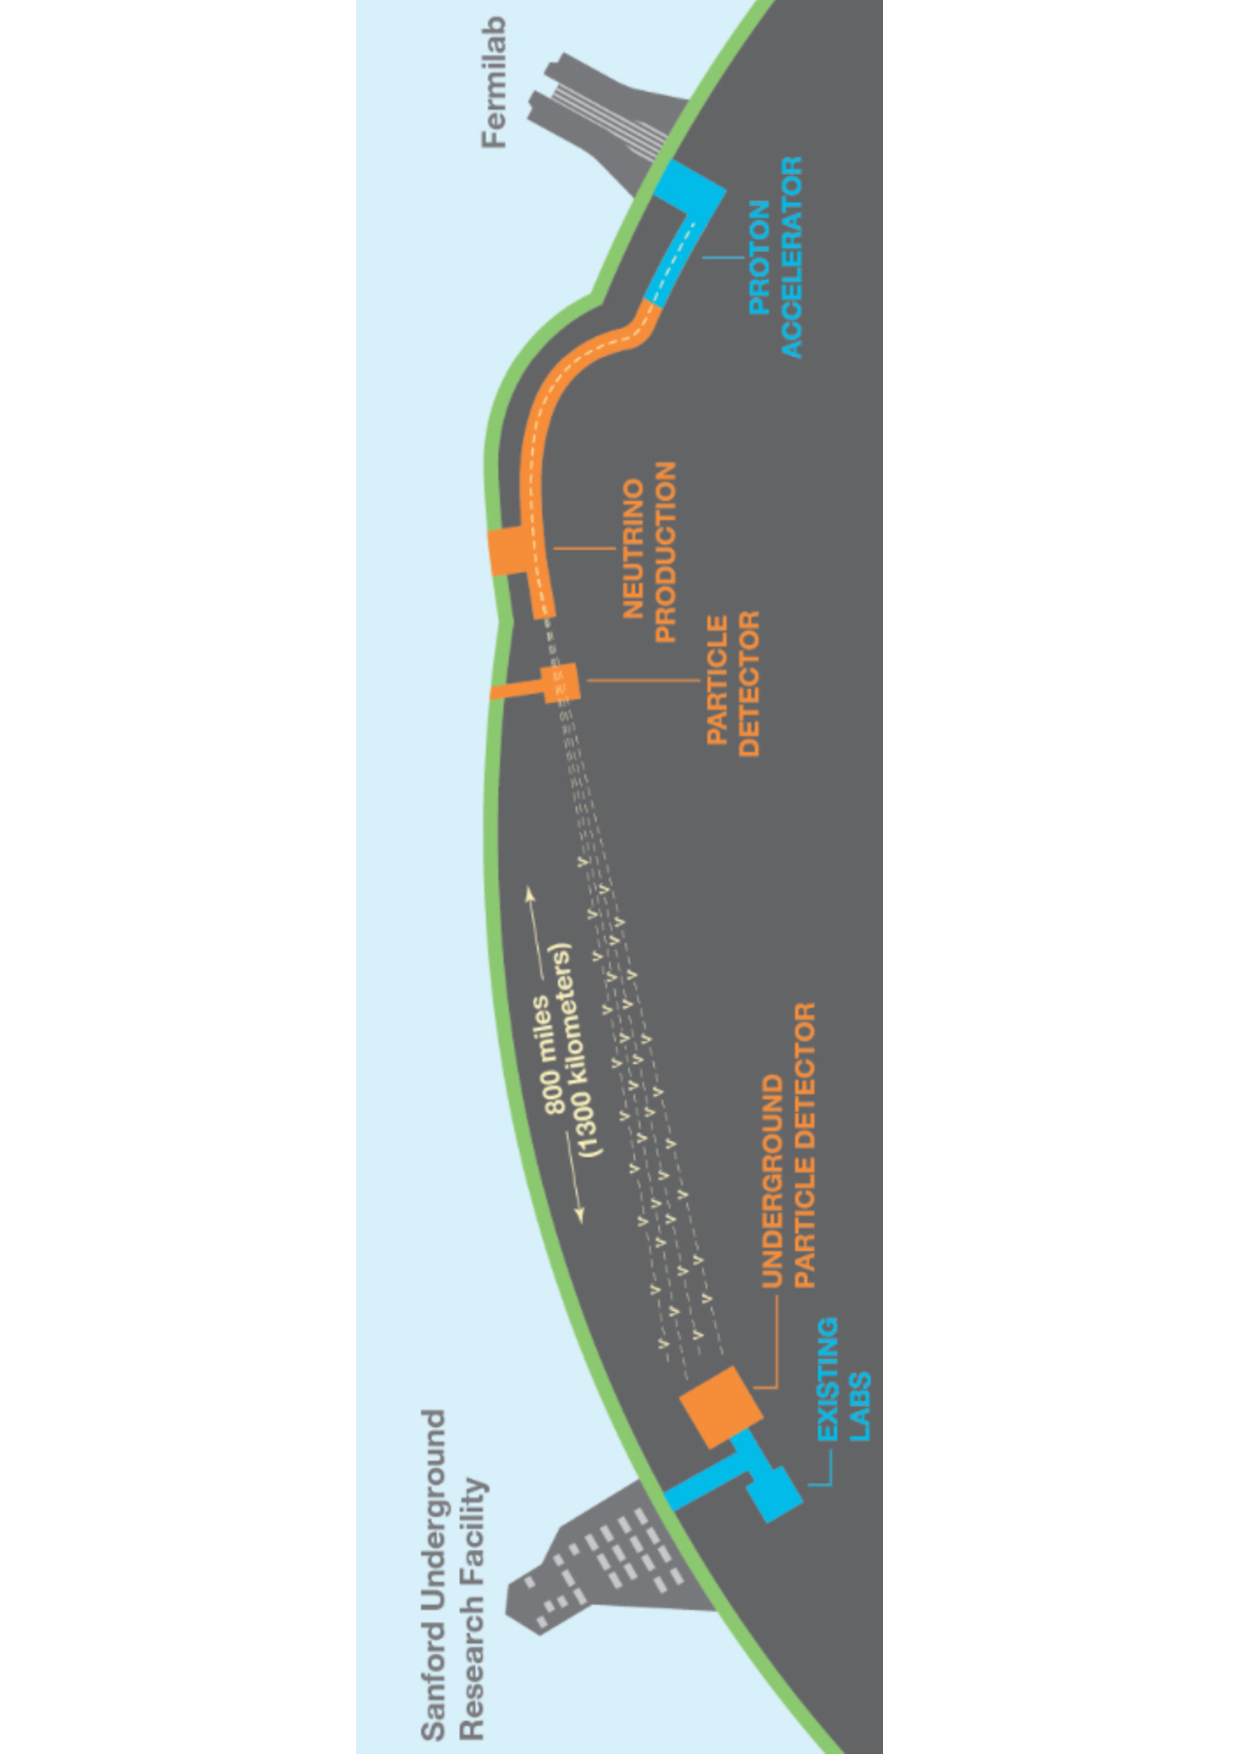
\includegraphics[width=0.9\textwidth]{DUNESchematic}
  \caption[A representation of the DUNE experimental setup]
          {A representation of the DUNE experimental setup. Fermilab, the host lab is shown on the right. The neutrino beam will be produced at Fermilab, and a high resolution near detector will also be located there. SURF is shown on the left, it is 1300~km away from Fermilab, and the far detector will be located there. Objects in orange need to be built during the lifetime of the experiment, whilst objects in blue already exist. The figure is not to scale, and is taken from~\citep{DUNECDR_V1}.}
  \label{fig:DUNESchematic}
\end{figure}

%********************************** %Second Section  *************************************
\section{The single phase detector design} \label{sec:DUNEDetector_SP}
As the work presented in this thesis has been performed on a prototype of the single phase design (Chapters~\ref{chap:Cameras},~\ref{chap:35tonSim} and~\ref{chap:35tonData}), and a simulation of the FD single phase design (Chapter~\ref{chap:FDSims}), the DUNE FD single phase design will be briefly described below. As no work has been performed in relation to the two phase design, no information will be presented concerning this design. Detailed descriptions of both the single and two phase FD designs can be found in~\citep{DUNECDR_V4}. \\

In the single phase design, the charge generation, electron drift, and charge collection, all occur in the LAr. \textcolor{red}{This takes advantage of the low ionisation threshold for liquid Argon at only 23.6~$\pm$0.5~eV~\citep{Chepel:2012sj}. Upon ionisation a large fraction of the lowest energy electrons recombine with the ion produced in the interaction, however in higher energy ionisations additional electrons are produced by inelastic collisions. When electrons recombine they produce flashes of scintillation light with a mean wavelength of 128~nm, which can also be measured by photon detectors normally covered in wavelength shifting coatings. The strength of the applied electric field is chosen to optimise the amount of scintillation light produced, compared to the charge measured, as at very low fields little charge is collected; whilst at large electric fields very little scintillation light is produced. An electric field of 500~V~cm$^{-1}$ is normally chosen as a compromise between these two effects~citep{Chepel:2012sj}.}

As the charge collection occurs in the LAr, this means that all of the TPC structure, including the electronics, are submerged. The active volume of 14.1~kt, measuring 12 m high, 14.5 m wide (in the drift direction), and 58 m long (in the beam direction), is too big to be contained in a single TPC, and so many individual TPCs are required. This is because it is not practical to collect electrons after they drift over many metres, or to construct an Anode Plane Assembly (APA) frame and Cathode Plane Assembly (CPA) frame across 10 metres or more. The mine shafts would also not be able to accommodate APA and CPA frames which were over 10 metres long or wide. This limit on size also affects the material used to make the cryostat, and so it will be constructed using a stainless steel membrane design. This design is commonly used for liquefied natural gas storage and transport tanker ships, and so is an established technology. However, it had not been used in LArTPC experiments before the 35 ton prototype detector, described in Section~\ref{sec:The35tonDetector}. \\

The active volume of the DUNE FD is divided into 200 TPCs, each produced by applying voltages to APAs and CPAs, and contained within a field cage. Each TPC measures 6 m high, 3.6 m wide (in the drift direction), and 2.3 long (along the beam direction). The TPCs are arranged such that there are 4 TPCs across the width of the detector, 2 TPCs stacked vertically on top of each other, and 25 TPCs along the length of the detector, to give the full active volume size of 12 $\times$ 14.5 $\times$ 58 m$^3$. This experimental setup means that the detector is 58 m long in the beam direction, offering a large region where neutrinos interaction can occur. The total drift distance of 14.5 m is split into four TPCs which are 3.6 m wide. Two sets of these four TPCs along the width of the beam are stacked on top of each other to produce the full height of the detector. A diagram showing this cross section of the single phase design is shown in Figure~\ref{fig:DUNE_SP_Schem}, where there would be an additional 24 cross sections going into the page, identical to the one shown. \\

\begin{figure}
  \centering
  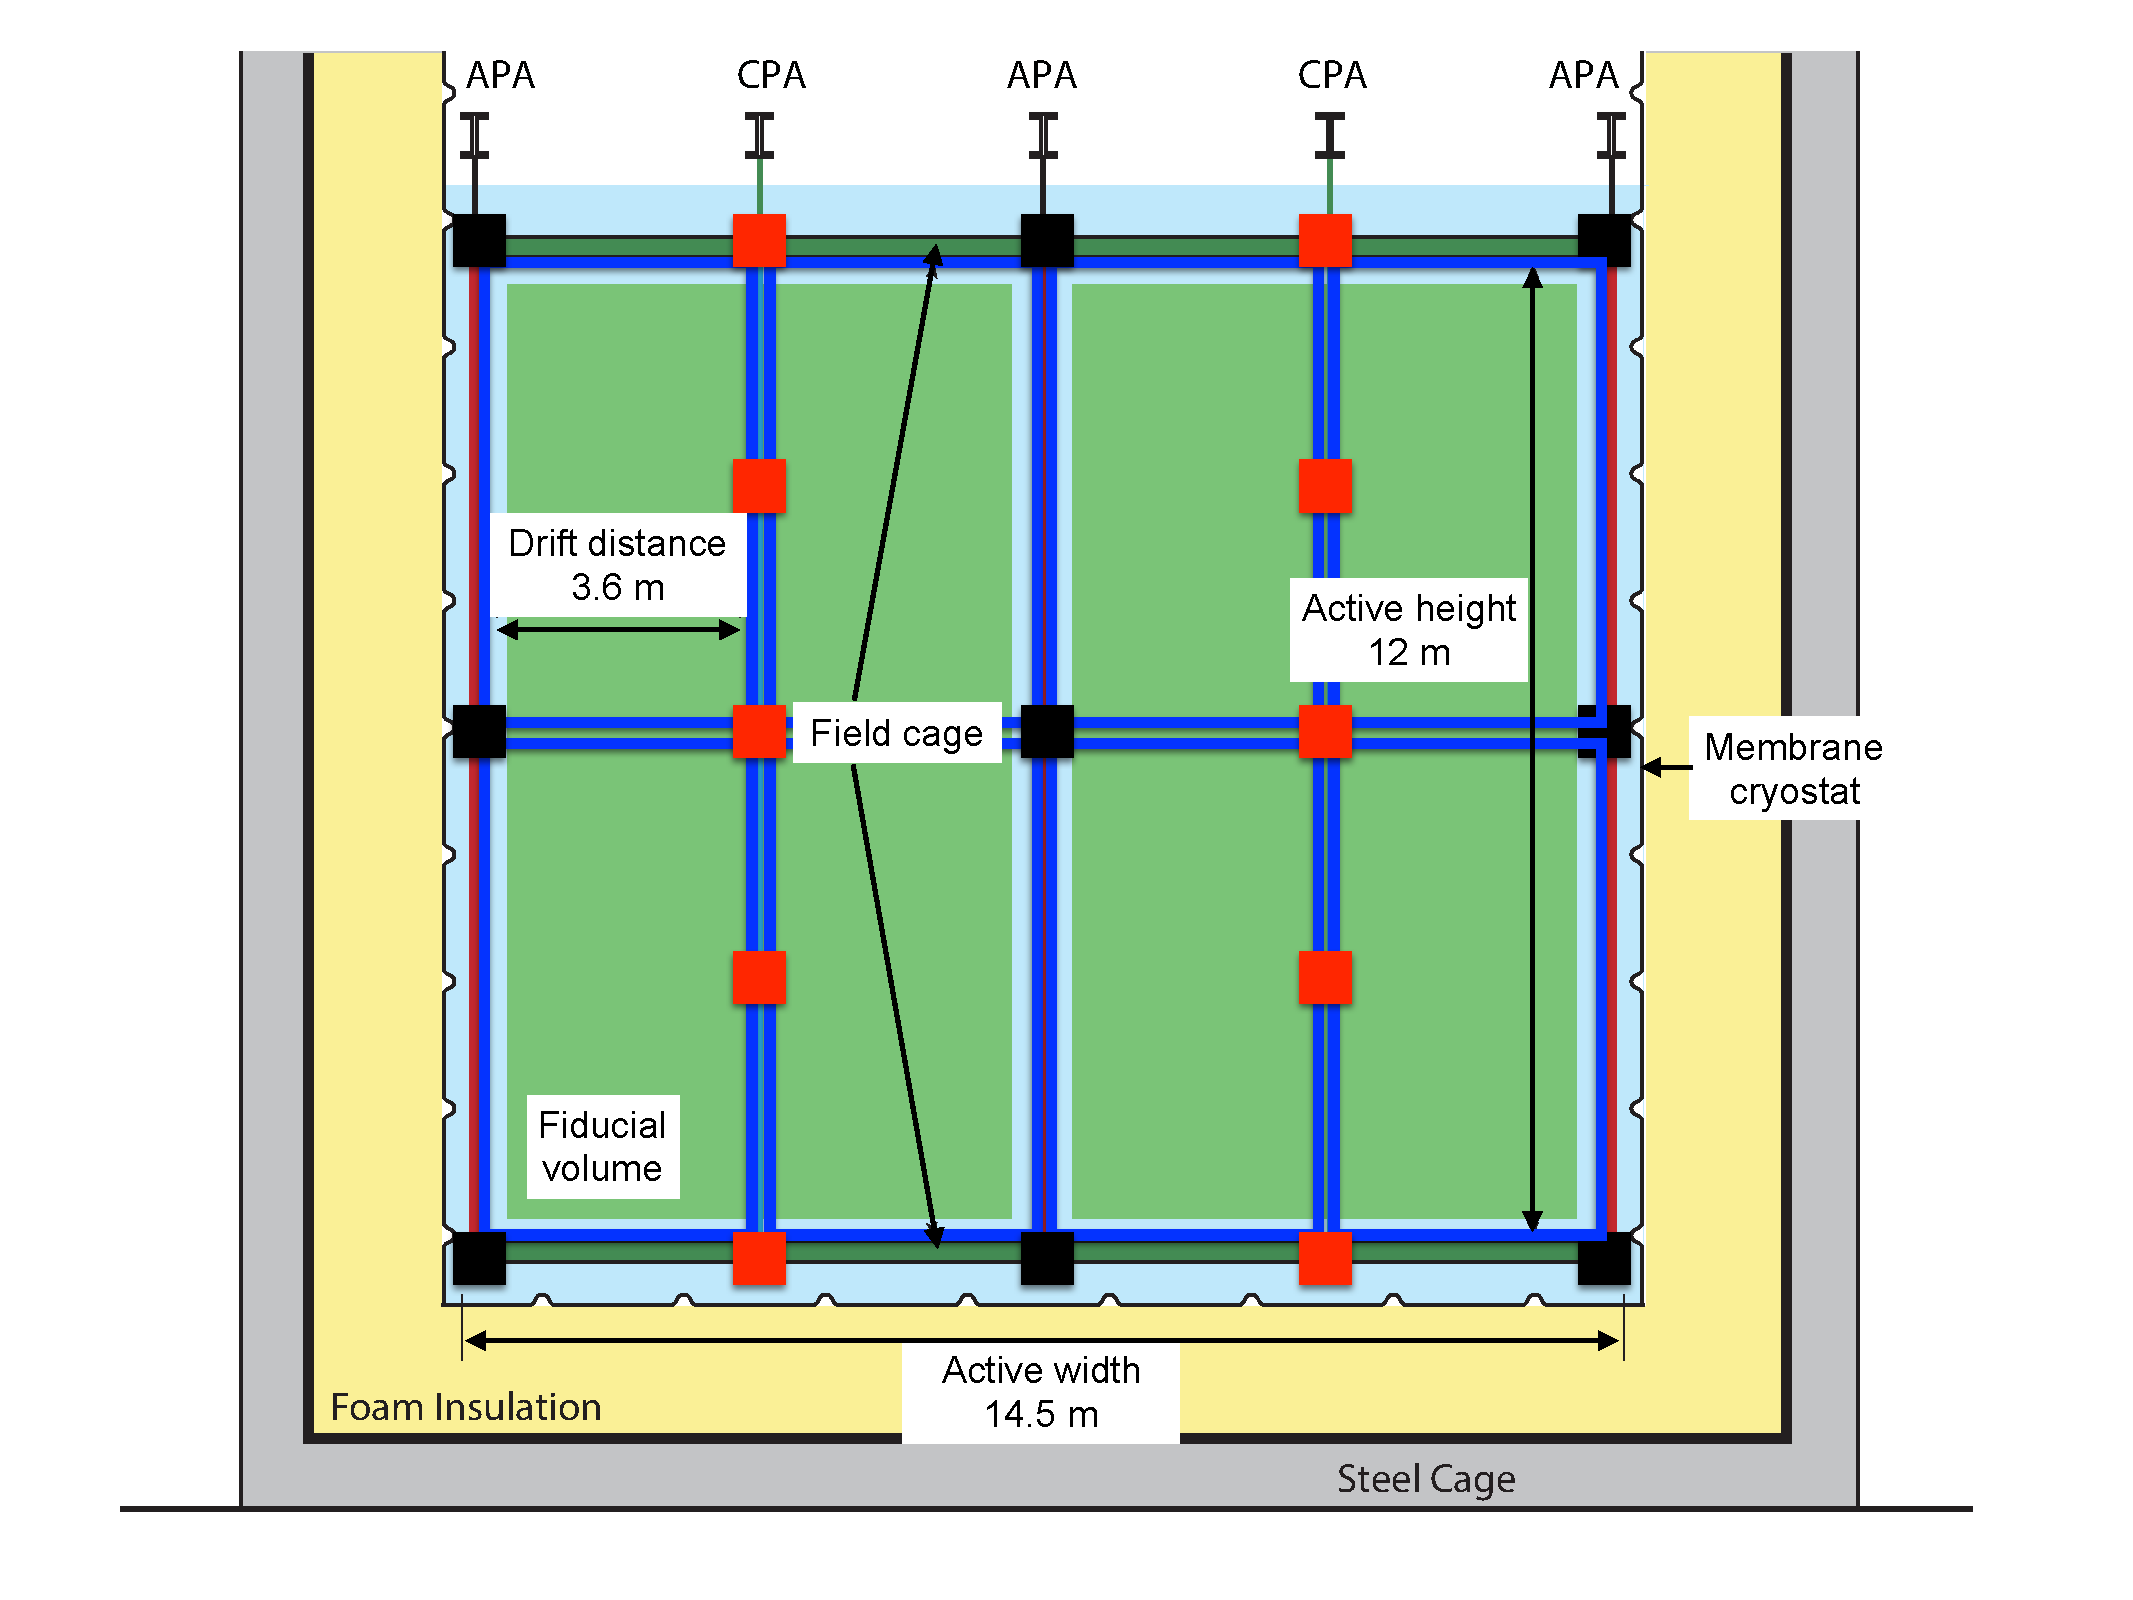
\includegraphics[width=\textwidth]{FarDetectorSchem}
  \caption[A cross section of the DUNE single phase detector design, showing 8 TPCs]
          {A cross section of the DUNE signal phase detector design, showing 8 TPCs. The cross section shown is looking along the beamline, such that the detector extends a total of 58 m into the page. The TPCs (blue squares) are bound between a pair of APAs and CPAs, and are surrounded by a field cage (green bar). The TPCs are ordered such that there are two TPCs vertically, and four horizontally, such that there are a total of 8 TPCs shown. The planes of APAs are made from two APAs (vertical gaps between black squares), and the planes of CPAs are made from four CPAs (vertical gaps between red squares). There are a total of 3 planes of APAs, and 2 planes of CPAs, ordered from left to right || APA | CPA | APA | CPA | APA ||. The fiducial volume of LAr (green) is shown included into the full volume of LAr (light blue), which is bounded by a membrane cryostat (thin black), contained in foam insulation (yellow), which is further contained in a steel cage (thick black) and a concrete structure (grey). In the full detector there will 24 more cross sections going into the page to produce a total of 200 TPCs. The figure has been modified from~\citep{DUNECDR_V4}.}
  \label{fig:DUNE_SP_Schem}
\end{figure}

As can be seen from Figure~\ref{fig:DUNE_SP_Schem} there are 3 planes of APAs and 2 planes of CPAs, ordered such that there is a CPA plane in between any two APA planes, and there are APA planes on the outer faces of the detector. The separation of the APA and CPA planes is 3.6 m, producing the 3.6 m drift of the detector design. The ionised electrons drift towards the APA planes, in an electric field of 500 V cm$^{-1}$, produced by the voltage difference between the CPA and APA. In total there will be 150 APA frames, and 200 CPA frames installed in each single FD module. \\

Each APA frame is instrumented on both sides with 4 wires planes, the properties of which are outlined in Table~\ref{tab:DUNE_SP_WP}. The first wire plane which a drifting electron would encounter is the grid plane (G), which acts to shield the other wire planes from distant moving charges and to make the field lines more stable near the wire planes. The grid plane wires are not read out. The next two wire planes are induction wire planes (U and V), and have a bias voltage such that electrons will not be collected on them, but will instead induce charge as they drift past. Finally, the fourth wire plane consists of collection plane wires (Z), which record the charge deposited by ionisation electrons. A grounded mesh behind the collection wires prevents the electric field around these wires being distorted by the metal frame of the APA. \\

\begin{table}
  \caption[The parameters of the wire planes in the DUNE FD single phase design]
          {The parameters of the wire planes in the DUNE FD single phase design.}
  \label{tab:DUNE_SP_WP}
  \centering
  \begin{tabular}{l c c c c}
    \toprule
    {Function}             & {Orientation ($^{\circ}$)} & {Pitch (mm)} & Num. Wires & Bias Voltage (V) \\ 
    \midrule
    Grid (G)               & 0                          & 4.79         & 960        & -655 \\
    
    1$^{st}$ induction (U) & 35.7                       & 4.67         & 800        & -365 \\
    
    2$^{nd}$ induction (V) & -35.7                      & 4.67         & 800        & 0    \\
    
    Collection (Z)         & 0                          & 4.79         & 960        & 860 \\
    \bottomrule
  \end{tabular}
\end{table}

The induction plane wires are wrapped around the long edges of the APA frames. This means that on each APA frame there are two sets of grid and collection planes, one on each side of the APA, and two induction plane wires, both of which are sensitive to both sides of the APA. The wrapping of the induction plane wires means that readout electronics are only required at one of the short ends of the APAs. As the collection plane wires are only sensitive to particles in one TPC, they can can resolve which TPC a measured charge on an induction plane wire was deposited in. An illustration of the wire wrapping on one of the DUNE FD APA frames is shown in Figure~\ref{fig:FDWireWrap}. \\

\begin{figure}
  \centering
  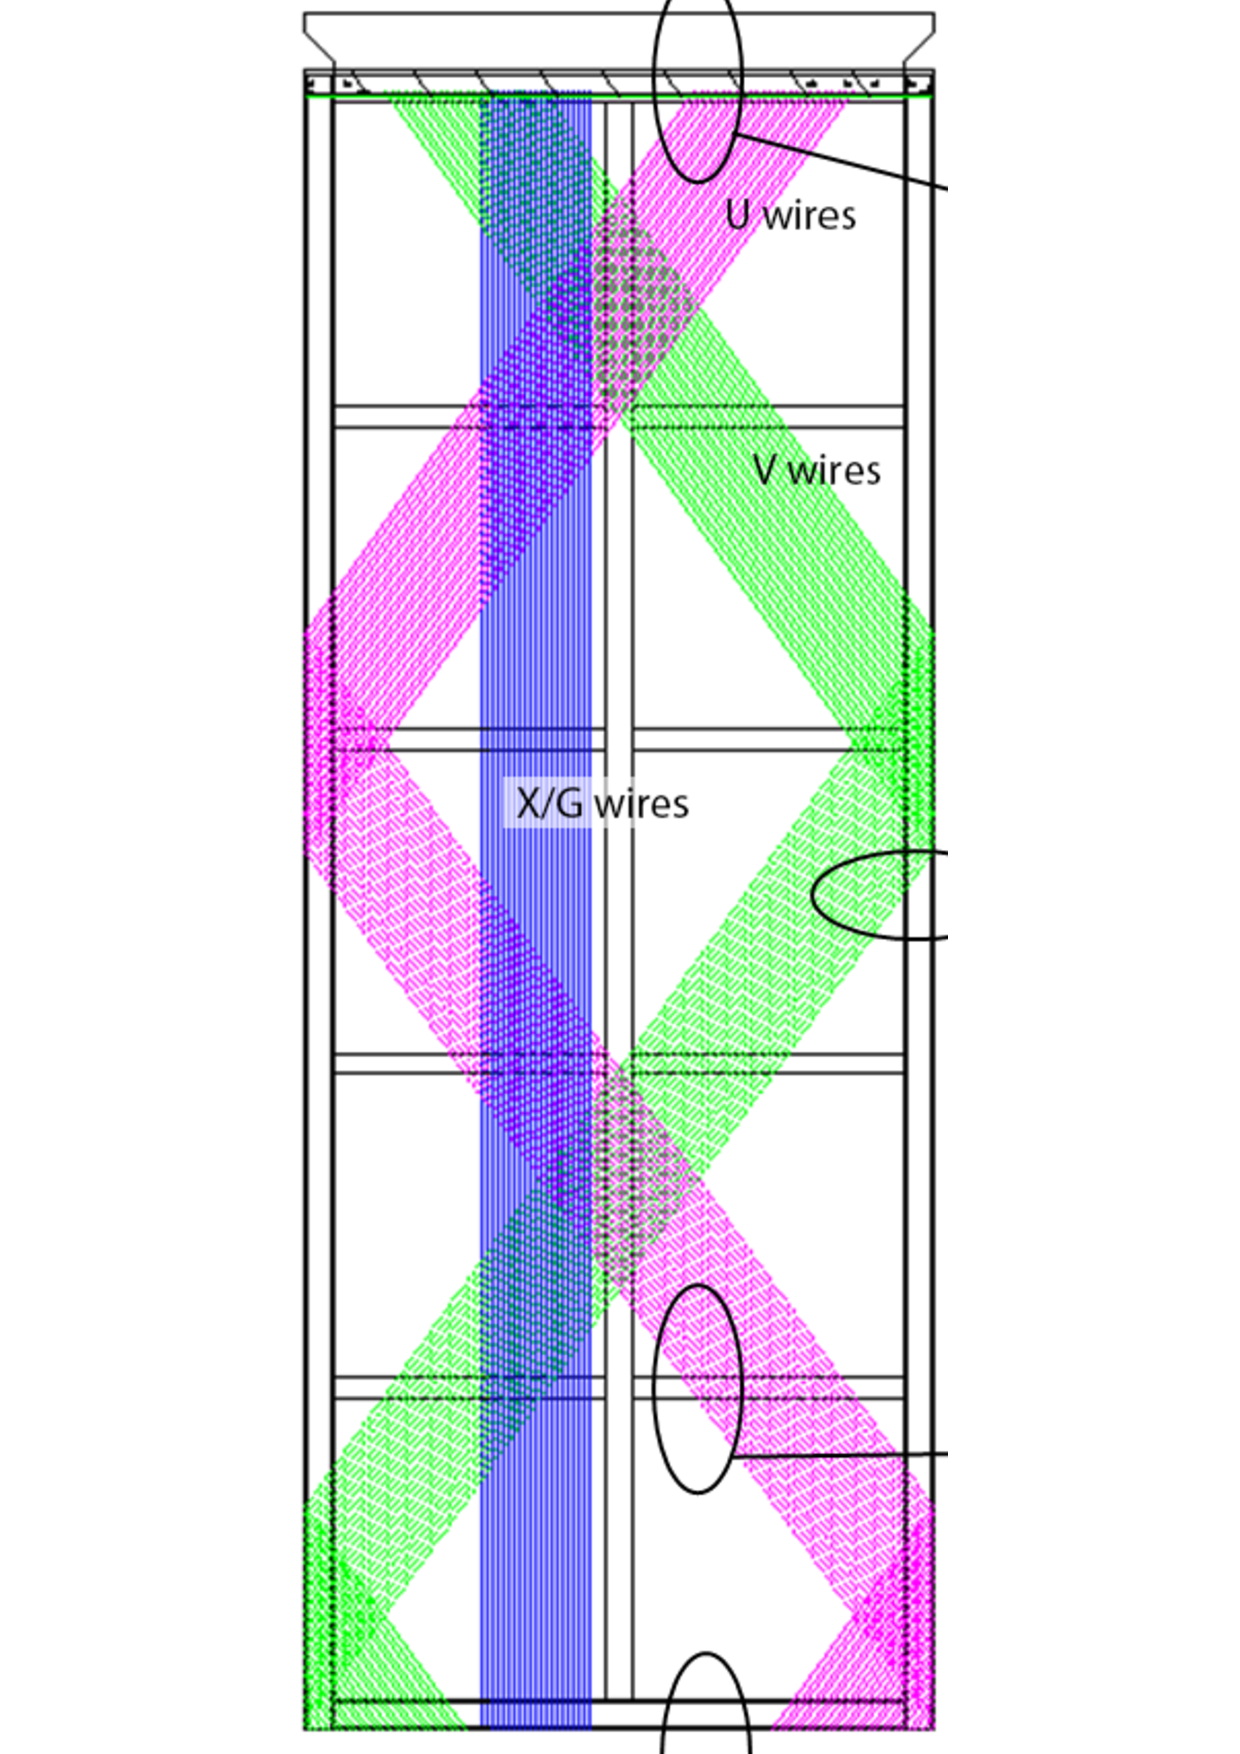
\includegraphics[width=0.4\textwidth]{tpc_apa_cross_sections}
  \caption[An illustration of the wire wrapping in the DUNE single phase design]
          {\textcolor{red}{An illustration of the wire wrapping in the DUNE single phase design. A small number of the wires in each plane are shown. The instrumented wire planes, in the order that the electrons drift past them, are shown as follows; the 1$^{st}$ induction plane (U) is red, the 2$^{nd}$ induction plane (V) is green, and the collection plane (Z) is blue. The grid plane (G), is in front of the 1$^{st}$ induction plane and is parallel to the collection plane. The figure is modified from~\citep{DUNECDR_V4}.}}
  \label{fig:FDWireWrap}
\end{figure}

It is also envisioned that there will be a system of Photon Detectors (PDs), to measure interaction times of both beam, and non-beam, events. An individual PD will be comprised of a light guide, and 12 Silicon PhotoMultipliers (SiPMs). Each APA frame will contain 10 equally spaced PDs, which will be between the two planes of grounded mesh. The PDs will use a wavelength shifter on the surface of the light guide, to convert the 128 nm scintillation photons from the LAr, to photons with a wavelength of 430 nm. This wavelength shifted light will be collected by the SiPMs. The front end electronics for the SiPMs will reside outside of the cryostat, where a SiPM Signal Processor (SSP) digitises the signals from the SiPMs. \\

%********************************** %Third Section  *************************************
\section{The physics capabilities of DUNE} \label{sec:DUNEPhys}%Section - X.2
DUNE hopes to be able to deliver a wide ranging physics programme. These topics include, but are not limited to, precision measurements of neutrino oscillation physics, discussed in Section~\ref{sec:DUNEPhys_Neut}, and searching for nucleon decay in several important decay modes, discussed in Section~\ref{sec:DUNE_NDK}. There are also additional physics goals\textcolor{red}{, such as searches for supernova neutrinos,} which are briefly outlined in Section~\ref{sec:DUNE_Other}. \\

%********************************** % 3.1 Section  *************************************
\subsection{Neutrino physics} \label{sec:DUNEPhys_Neut} %Section - X.2.1
The primary goals of DUNE concern neutrino physics, where many of these ideas were introduced in Section~\ref{sec:NeutPhys}, and are~\citep{DUNECDR_V2}:
\begin{itemize}
\item Determine the neutrino mass hierarchy.
\item Measure the charge-parity (CP) violating phase - $\delta_{CP}$.
\item Make precision measurements of the neutrino mixing parameters, such as $\theta_{13}$, $\theta_{23}$, and $\Delta m^{2}_{31}$.
\end{itemize}
There are also secondary physics goals concerning neutrino physics, these include:
\begin{itemize}
\item Measuring neutrino oscillations using atmospheric neutrinos.
\item Measuring a wide range of neutrino cross-sections, using the ND.
\item Measuring nuclear effects, particularly neutrino final-state interactions, using the ND.
\end{itemize}
The beam exposure as a function of time which DUNE will receive is shown in Table~\ref{tab:DUNEExposure}, and is important when considering the figures presented below. \\

\begin{table}
\caption[The beam exposure in units in units of~kt$\cdot$MW$\cdot$years, as a function of time, assuming a staged DUNE construction]
        {The beam exposure in units in units of~kt$\cdot$MW$\cdot$years, as a function of time, assuming a staged DUNE construction. This table uses the fiducial mass of the detector (10~kt), the power of the initial proton beam (1.2-2.4~MW), and the time that the detector is exposed to the beam (years). The table is taken from~\citep{Elizabeth_01_17}.}
\centering
\label{tab:DUNEExposure}
\begin{tabular}{c c}
\toprule
{Exposure (kt$\cdot$MW$\cdot$years)} & {Exposure (years)} \\
\midrule
171                      & 5 \\

300                      & 7 \\

556                      & 10 \\

984                      & 15 \\
\bottomrule
\end{tabular}
\end{table}

As presented in Section~\ref{sec:NeutPhys}, both the matter effect, and $\delta_{CP}$ introduce an asymmetry between neutrino and anti-neutrino oscillations. As the matter effect is caused by the difference in the presence/absence of electrons/positrons in the Earth, it increases with distance. The result of this is that for baselines longer than approximately 1000~km the two effects can be resolved~\citep{Bass:2013vcg}. For this reason DUNE will have a baseline of 1300~km so that it is able to unambiguously determine the neutrino mass hierarchy, and determine $\delta_{CP}$~\citep{Diwan:2004bt}. \\

Figure~\ref{fig:DUNEOscillProb} shows the oscillation probabilities of $\nu_{\mu} \rightarrow \nu_{e}$ for both neutrino and anti-neutrino modes at a baseline of 1300~km. The reason for requiring a broadband neutrino beam at this baseline is clearly apparent, as it can be seen that whilst the energy of the first neutrino oscillation maximum is relatively unaffected by the value of $\delta_{CP}$, the energies of the higher oscillation maxima are strongly affected. It is therefore vital that DUNE is able to accurately measure the rate of $\nu_e$ appearance at the lowest energies of the neutrino beam. It can also be seen that there are large differences in the expected oscillation probabilities for neutrinos and anti-neutrinos. Therefore, in order to measure the effect of $\delta_{CP}$, the neutrino beam will have to be able to operate in both neutrino and anti-neutrino mode. \\

\begin{figure}
  \centering 
  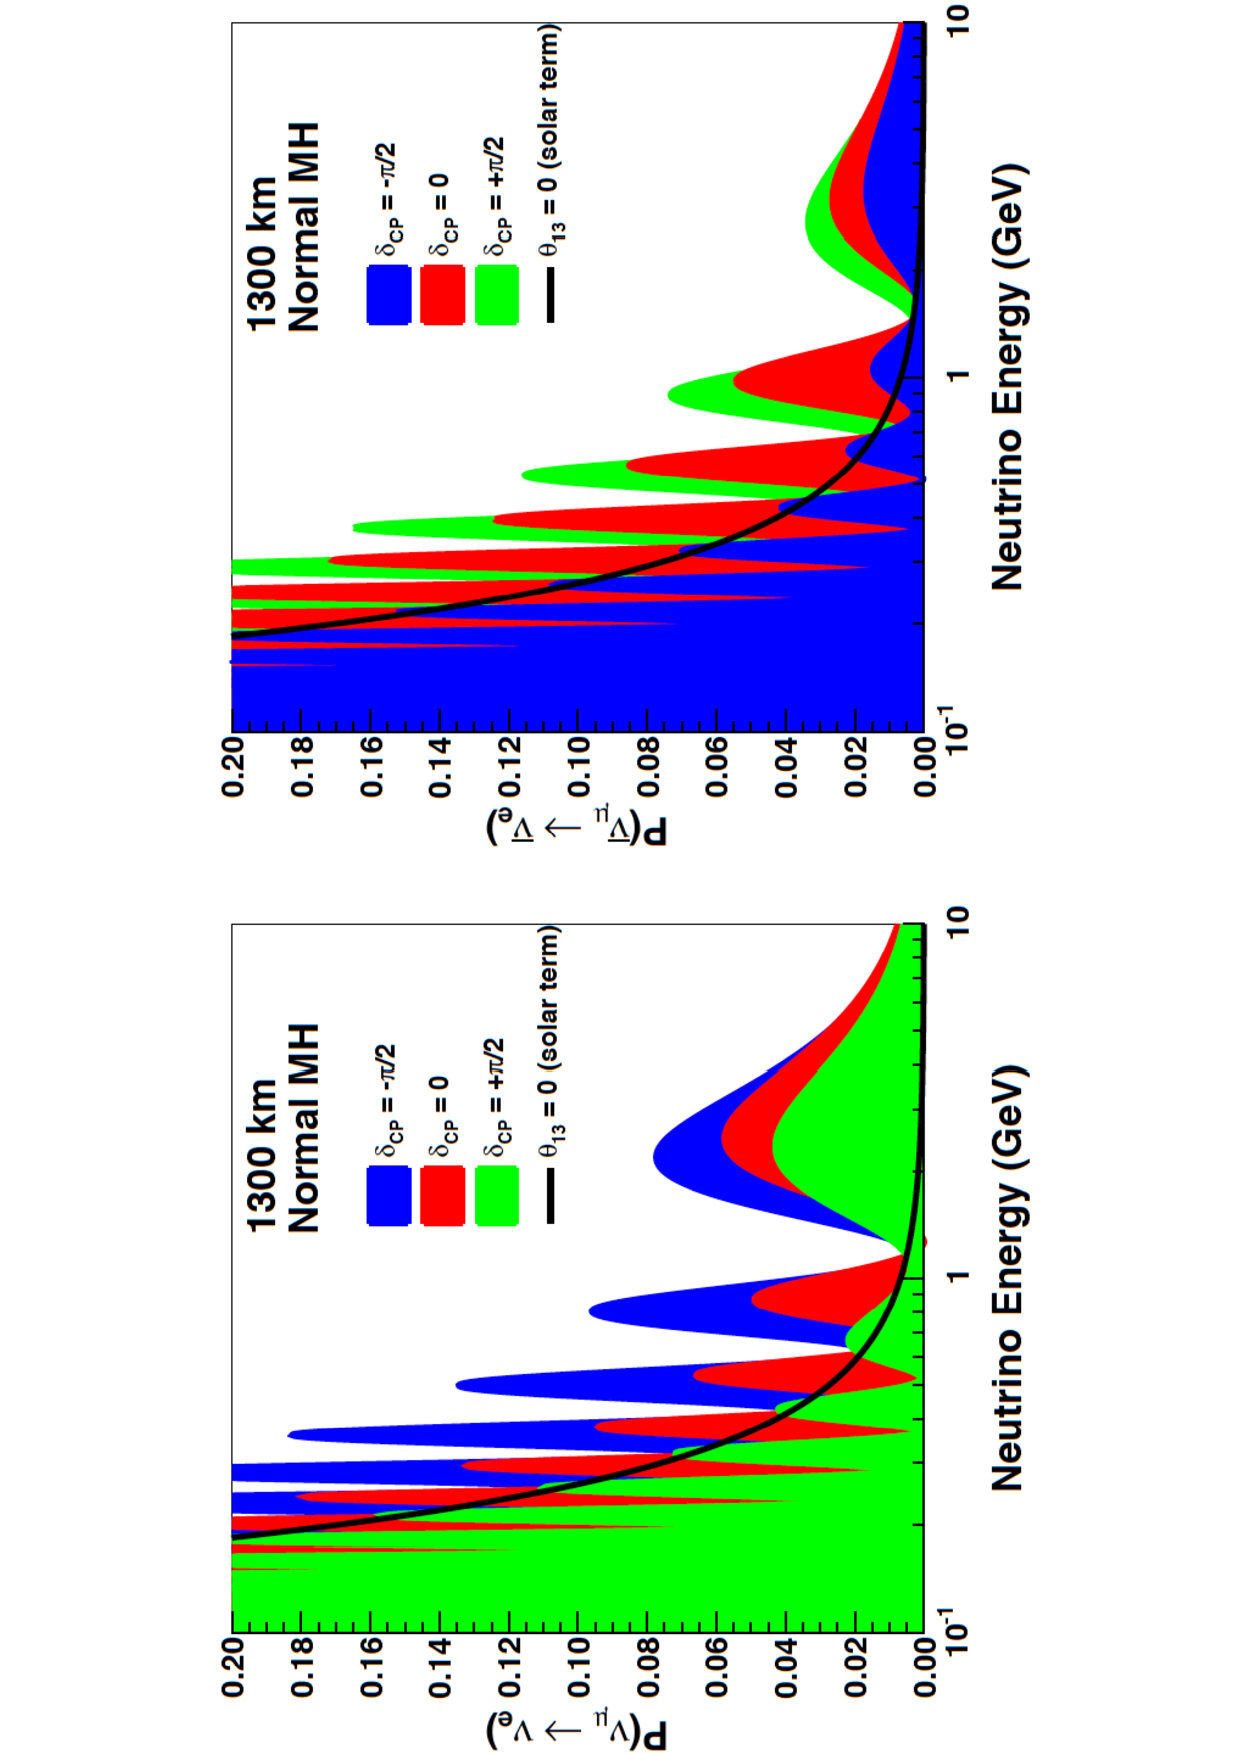
\includegraphics[width=0.9\textwidth]{DUNEOscillProb}
  \caption[The $\nu_e$ appearance probability at 1300~km as a function of neutrino energy, for a range of values of $\delta_{CP}$]
          {The $\nu_e$ appearance probability at 1300~km as a function of neutrino energy, for a range of values of $\delta_{CP}$. Left: the oscillation probability for neutrinos. Right:, the oscillation probability for anti-neutrinos. Both figures assume normal mass hierarchy ($\nu_1$ is the lightest state). The probabilities for different values of $\delta_{CP}$ are shown, $\delta_{CP} = -\pi/2$ (blue), $\delta_{CP} = 0$ (red), $\delta_{CP} = \pi/2$ (green). The figure is taken from~\citep{DUNECDR_V2}.}
  \label{fig:DUNEOscillProb}
\end{figure}

Figures~\ref{fig:DUNEMassHierarchy} and~\ref{fig:DUNECPViolation} show the DUNE sensitivities to the mass hierarchy, and the value of $\delta_{CP}$, with beam exposures corresponding to 7 and 10 years worth of data taking~\citep{Elizabeth_01_17}. These beam exposures are calculated given the phased approach to DUNE which was outlined in Table~\ref{tab:DUNEExposure}, meaning that a beam exposure of 7 years corresponds to a beam exposure 300~kt$\cdot$MW$\cdot$years, whilst a beam exposure of 10 years corresponds to a beam exposure of 556~kt$\cdot$MW$\cdot$years. The best fit values from NuFit 2016~\citep{NuFit2016} are used when making these figures, and equal running in neutrino and antineutrino mode is assumed. Figures~\ref{fig:DUNEOctantDetermination},~\ref{fig:DUNETheta23Res},~\ref{fig:DUNETheta13Res} and~\ref{fig:DUNEDeltaMRes} are taken from the CDR~\citep{DUNECDR_V2}, and show \textcolor{red}{how accurately given mixing parameters can be determined for increasing exposures.} \\

Figure~\ref{fig:DUNEMassHierarchy} shows the significance with which DUNE will be able to determine the neutrino mass hierarchy, for all values of $\delta_{CP}$. It can be seen that the mass hierarchy can be determined with a significance of $\sqrt{\overline{\Delta{\chi^2}}}$ = 5, for all values of $\delta_{CP}$ after 7 years of data taking. It can also be seen that the mass hierarchy can be more conclusively determined if it is inverted. \\

\begin{figure}
  \centering
  \begin{subfigure}{0.49\textwidth}
    \centering
    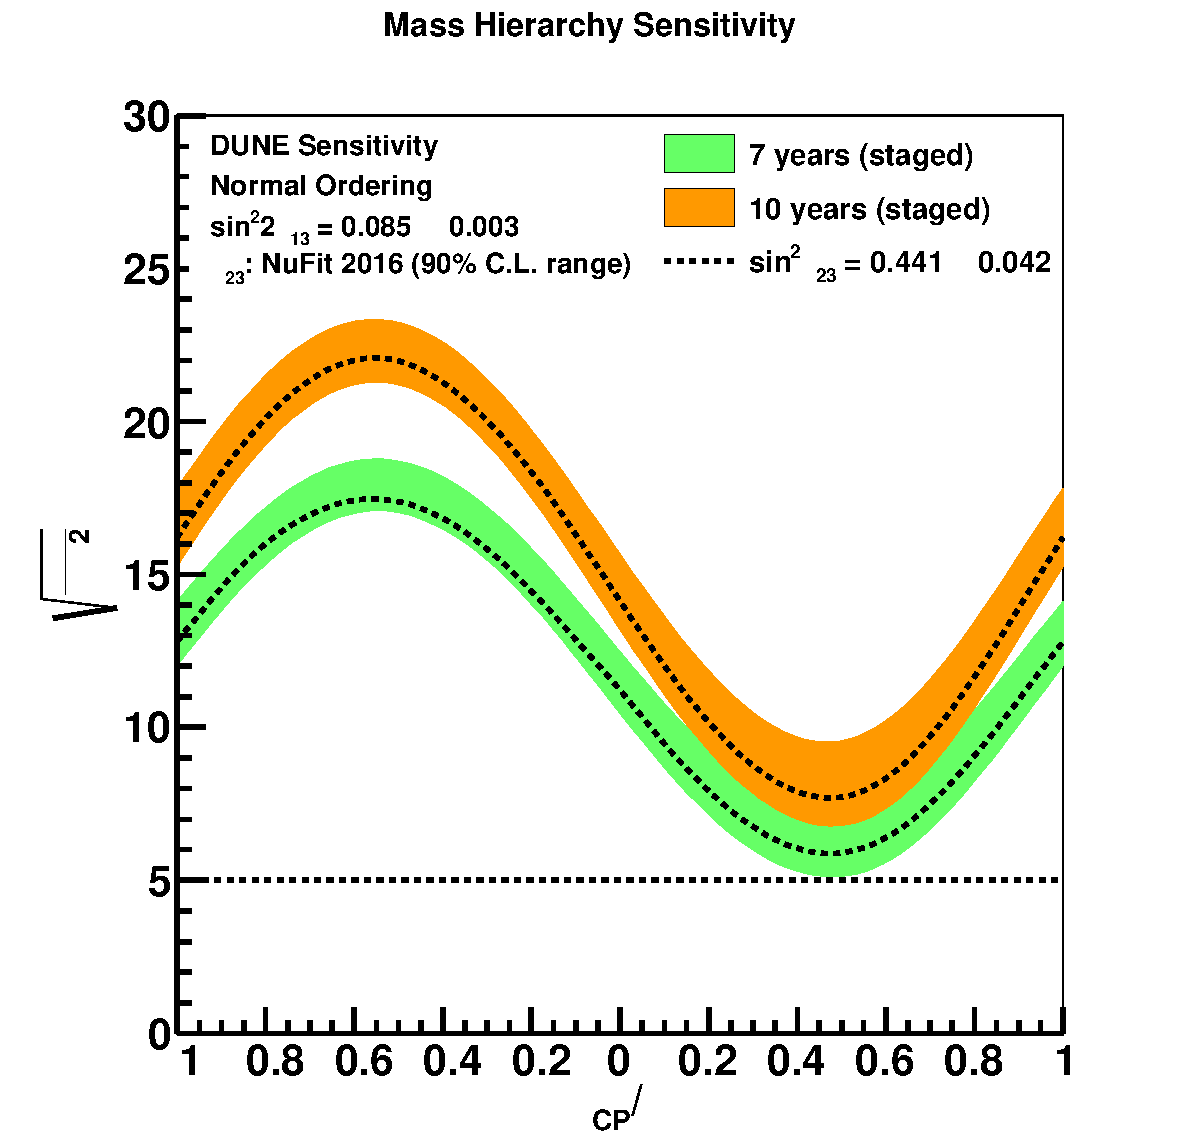
\includegraphics[width=\textwidth]{mh_two_exps_th23band_no_2017}
    \caption{Normal ordering.}
  \end{subfigure}%
  \begin{subfigure}{0.49\textwidth}
    \centering
    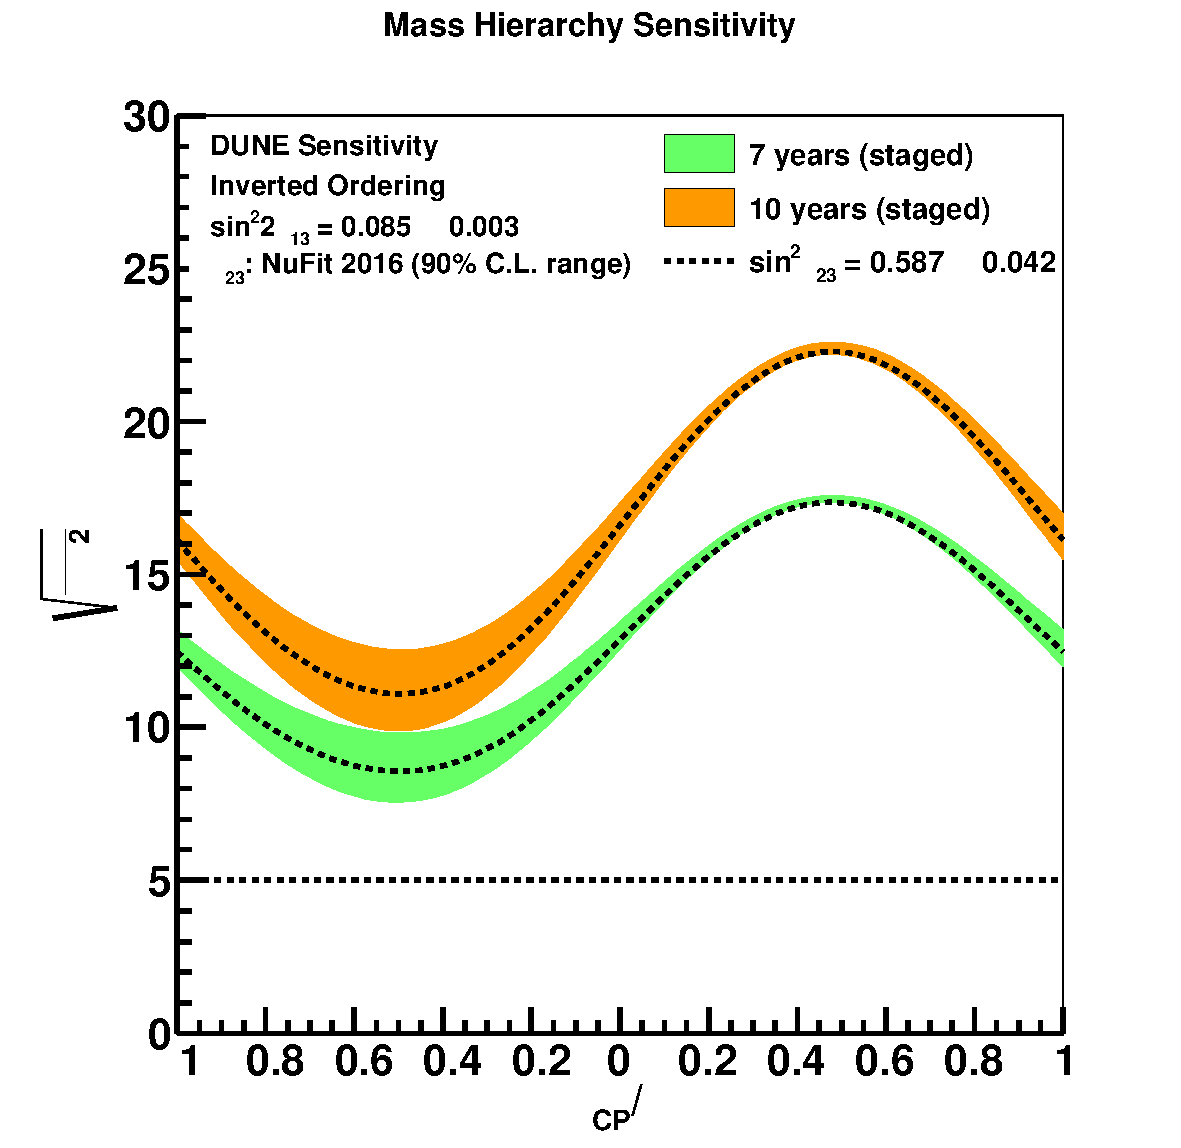
\includegraphics[width=\textwidth]{mh_two_exps_th23band_io_2017}
    \caption{Inverted ordering.}
  \end{subfigure}
  \caption[The significance with which DUNE will be able to determine the neutrino mass hierarchy, for all values of $\delta_{CP}$]
          {The significance with which DUNE will be able to determine the neutrino mass hierarchy, for all values of $\delta_{CP}$. Left: the sensitivity assuming normal ordering. Right: the sensitivity assuming inverted ordering. The shaded region shows the range of sensitivities for the 90\% confidence level range for $\theta_{23}$ values, the dashed line shows the sensitivity for the NuFit central value of $\theta_{23}$. The figure is taken from~\citep{DUNE2335}.}
  \label{fig:DUNEMassHierarchy}
\end{figure}

Figure~\ref{fig:DUNECPViolation} shows the significance with which DUNE will be able to determine the value of $\delta_{CP}$. It can be seen that even with 10 years worth of data, there are regions where the value of $\delta_{CP}$ cannot be determined accurately because of the complex phase being 0 when $\delta_{CP}$ is equal to $-\pi$, 0, or $\pi$. Therefore, for values of $\delta_{CP}$ around these values, the significance to which $\delta_{CP}$ can be determined approaches 0. As such, even at very large beam exposures of over 800~kt$\cdot$MW$\cdot$years, corresponding to around 13 years of data taking according to Table~\ref{tab:DUNEExposure}, only 75\% of the $\delta_{CP}$ values can be determined to a significance of 3$\sigma$~\citep{DUNE2401}. However, even with a relatively modest exposure of 150~(550)~kt$\cdot$MW$\cdot$years, DUNE can determine the value of $\delta_{CP}$ for over 50\% of the range for $\delta_{CP}$ to a significance of 3$\sigma$ (5$\sigma$)~\citep{DUNE2401}. This shows that should the value of $\delta_{CP}$ be close to a CP-conserving case, it would be very difficult to determine it. However, if it is far away from these values, DUNE could make a measurement, with a significance of over 5$\sigma$, in a matter of years. \\

\begin{figure}
  \centering
  \begin{subfigure}{0.49\textwidth}
    \centering
    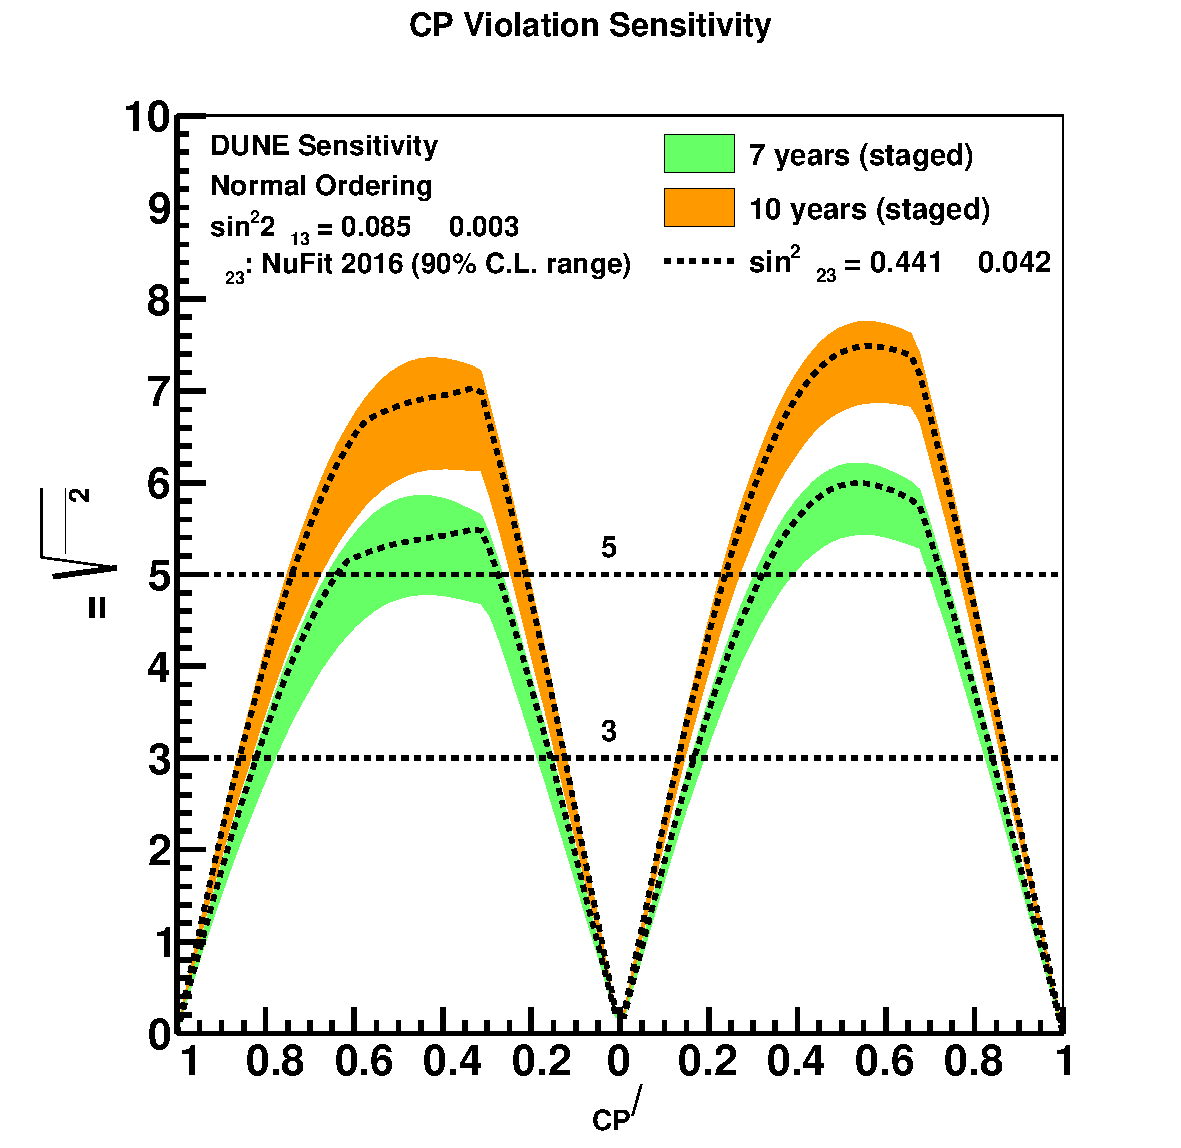
\includegraphics[width=\textwidth]{cpv_two_exps_th23band_no_2017}
    \caption{Normal ordering.}
  \end{subfigure}%
  \begin{subfigure}{0.49\textwidth}
    \centering
    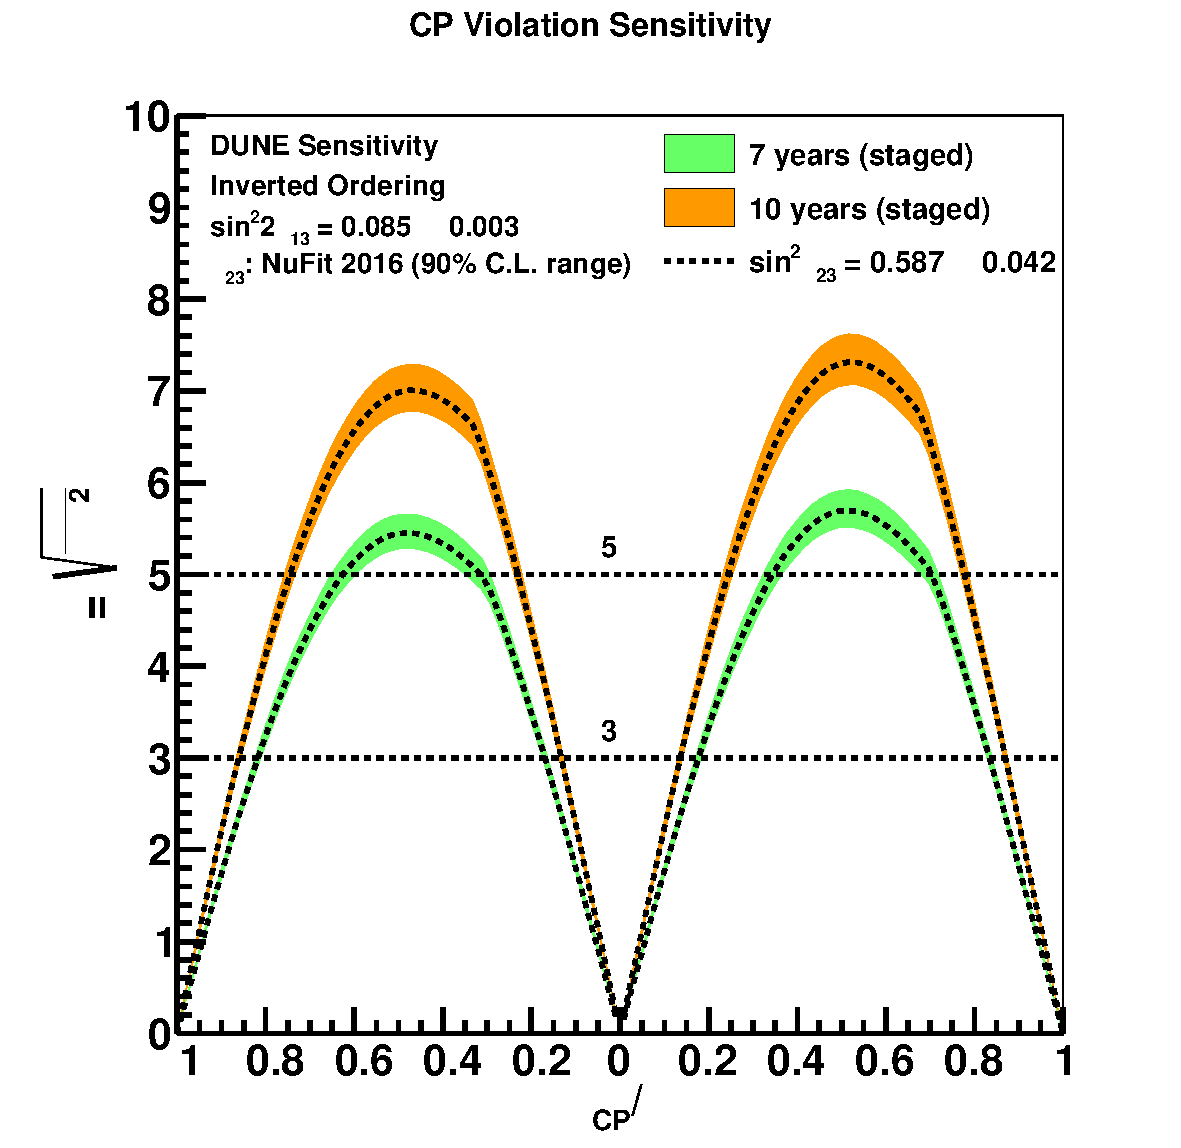
\includegraphics[width=\textwidth]{cpv_two_exps_th23band_io_2017}
    \caption{Inverted ordering.}
  \end{subfigure}
  \caption[The significance with which DUNE will be able to determine the value of $\delta_{CP}$, for all values of $\delta_{CP}$]
          {The significance with which DUNE will be able to determine the value of $\delta_{CP}$, for all values of $\delta_{CP}$. Left: the sensitivity assuming the normal ordering. Right: the sensitivity assuming inverted inverted. The shaded region shows the range of sensitivities for the 90\% confidence level range for $\theta_{23}$ values, the dashed line shows the sensitivity for the NuFit central value of $\theta_{23}$. The figure is taken from~\citep{DUNE2332}.}
  \label{fig:DUNECPViolation}
\end{figure}

Figure~\ref{fig:DUNECPViolationRes} shows the resolution to which $\delta_{CP}$ can be determined when the value of $\delta_{CP}$ is both maximally CP-violating ($\delta_{CP}$ = 90$^{\circ}$), and when it is CP-conserving ($\delta_{CP}$ = 0$^{\circ}$). Somewhat paradoxically, the resolution is better when $\delta_{CP}$ = 0$^{\circ}$. The reason for this, is that the region of values of $\delta_{CP}$ for which CP-violation would not be observed becomes increasingly small, as the beam exposure increases. This means that the resolution to which $\delta_{CP}$ can be determined increases. However, the more interesting result would be the one which supported $\delta_{CP}$ having a value which causes maximal CP-violation. \\

\begin{figure}
  \centering
  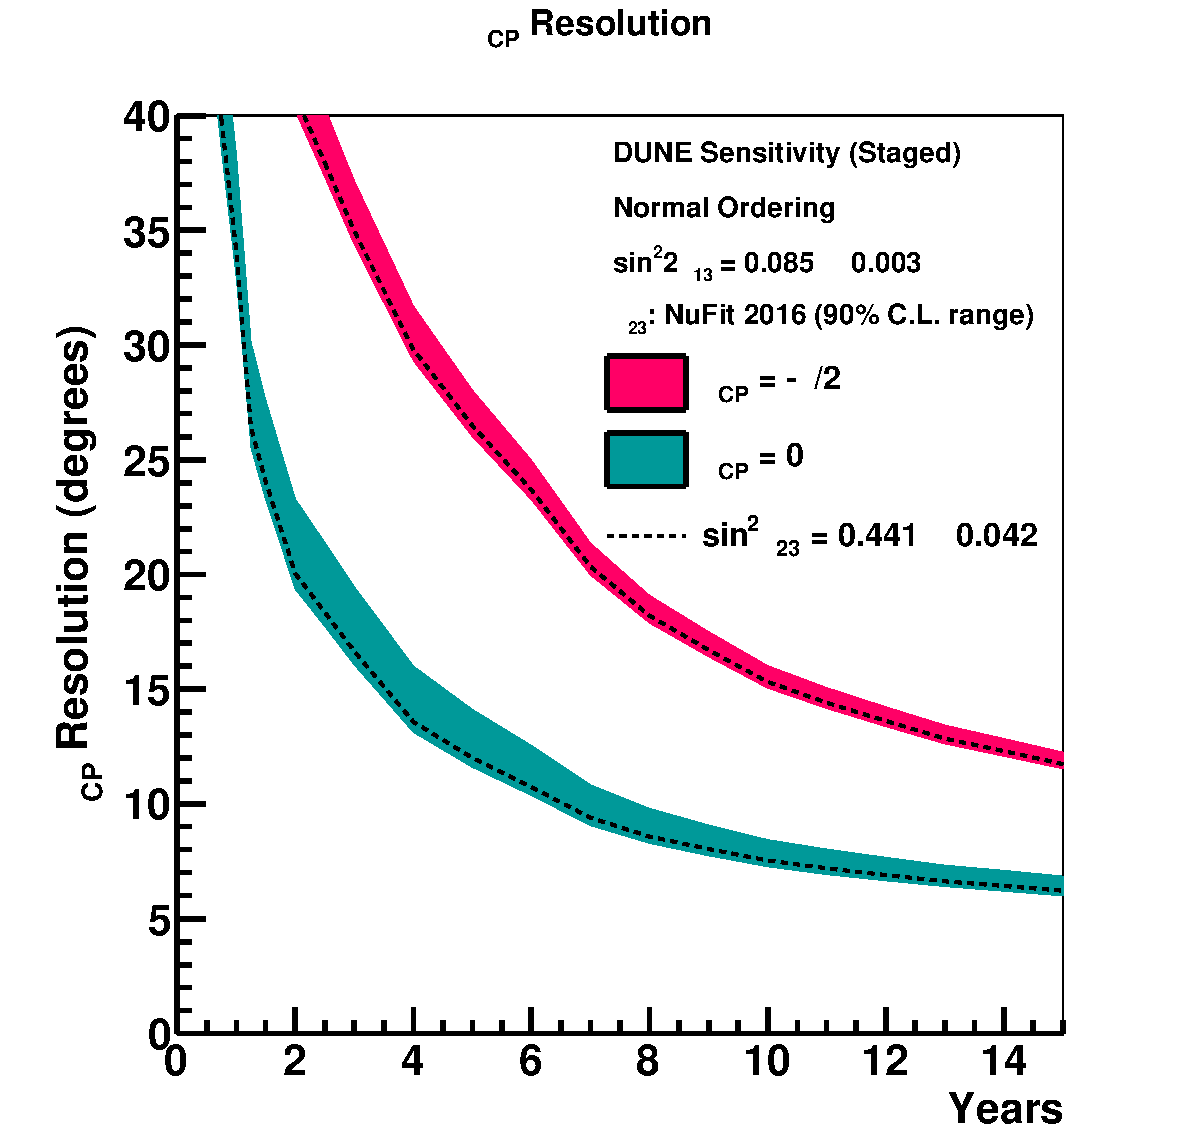
\includegraphics[width=0.5\textwidth]{resdcp_exp_staging_th23band_2017}
  \caption[The resolution with which DUNE will be able to determine the value of $\delta_{CP}$, for increasing beam exposures]
          {The resolution with which DUNE will be able to determine the value of $\delta_{CP}$, for increasing beam exposures (in years). Two bands are shown, one for a value of $\delta_{CP}$ which could cause maximal CP-violation ($\delta_{CP}$ = 90$^{\circ}$), and another where there would be no CP-violation ($\delta_{CP}$ = 0$^{\circ}$). A normal hierarchy is assumed, and the shaded region shows the range of sensitivities for the 90\% confidence level range for $\theta_{23}$ values. The dashed line shows the sensitivity for the NuFit central value of $\theta_{23}$. The figure is taken from~\citep{DUNE2377}.}
  \label{fig:DUNECPViolationRes}
\end{figure}

DUNE also aims to perform precision measurements of the neutrino mixing parameters in order to improve sensitivity to any physics beyond the standard thee-flavour oscillation model. As discussed in Section~\ref{sec:Theory_Exp}, the current best limit for the value of $\theta_{23}$ does not determine which octant it is in, specifically whether it is more than, or less than, 45$^{\circ}$. Determining the octant of $\theta_{23}$ is important, as, should it be found that $\theta_{23}$ is equal to 45$^{\circ}$, it would hint at an unknown symmetry. DUNE will determine the value of $\theta_{23}$ by combining measurements of $\nu_{\mu} \rightarrow \nu_{\mu}$ and $\nu_{\mu} \rightarrow \nu_{e}$, which are sensitive to $\sin^{2}2\theta_{23}$ and $\sin^2\theta_{23}$, respectively. Figure~\ref{fig:DUNEOctantDetermination} shows the significance to which the octant of $\theta_{23}$ can be determined for different values of $\theta_{23}$. Figure~\ref{fig:DUNETheta23Res} shows the resolution to which the value of $\sin^{2}\theta_{23}$ can be determined with increasing beam exposures. \\

\begin{figure}
  \centering
  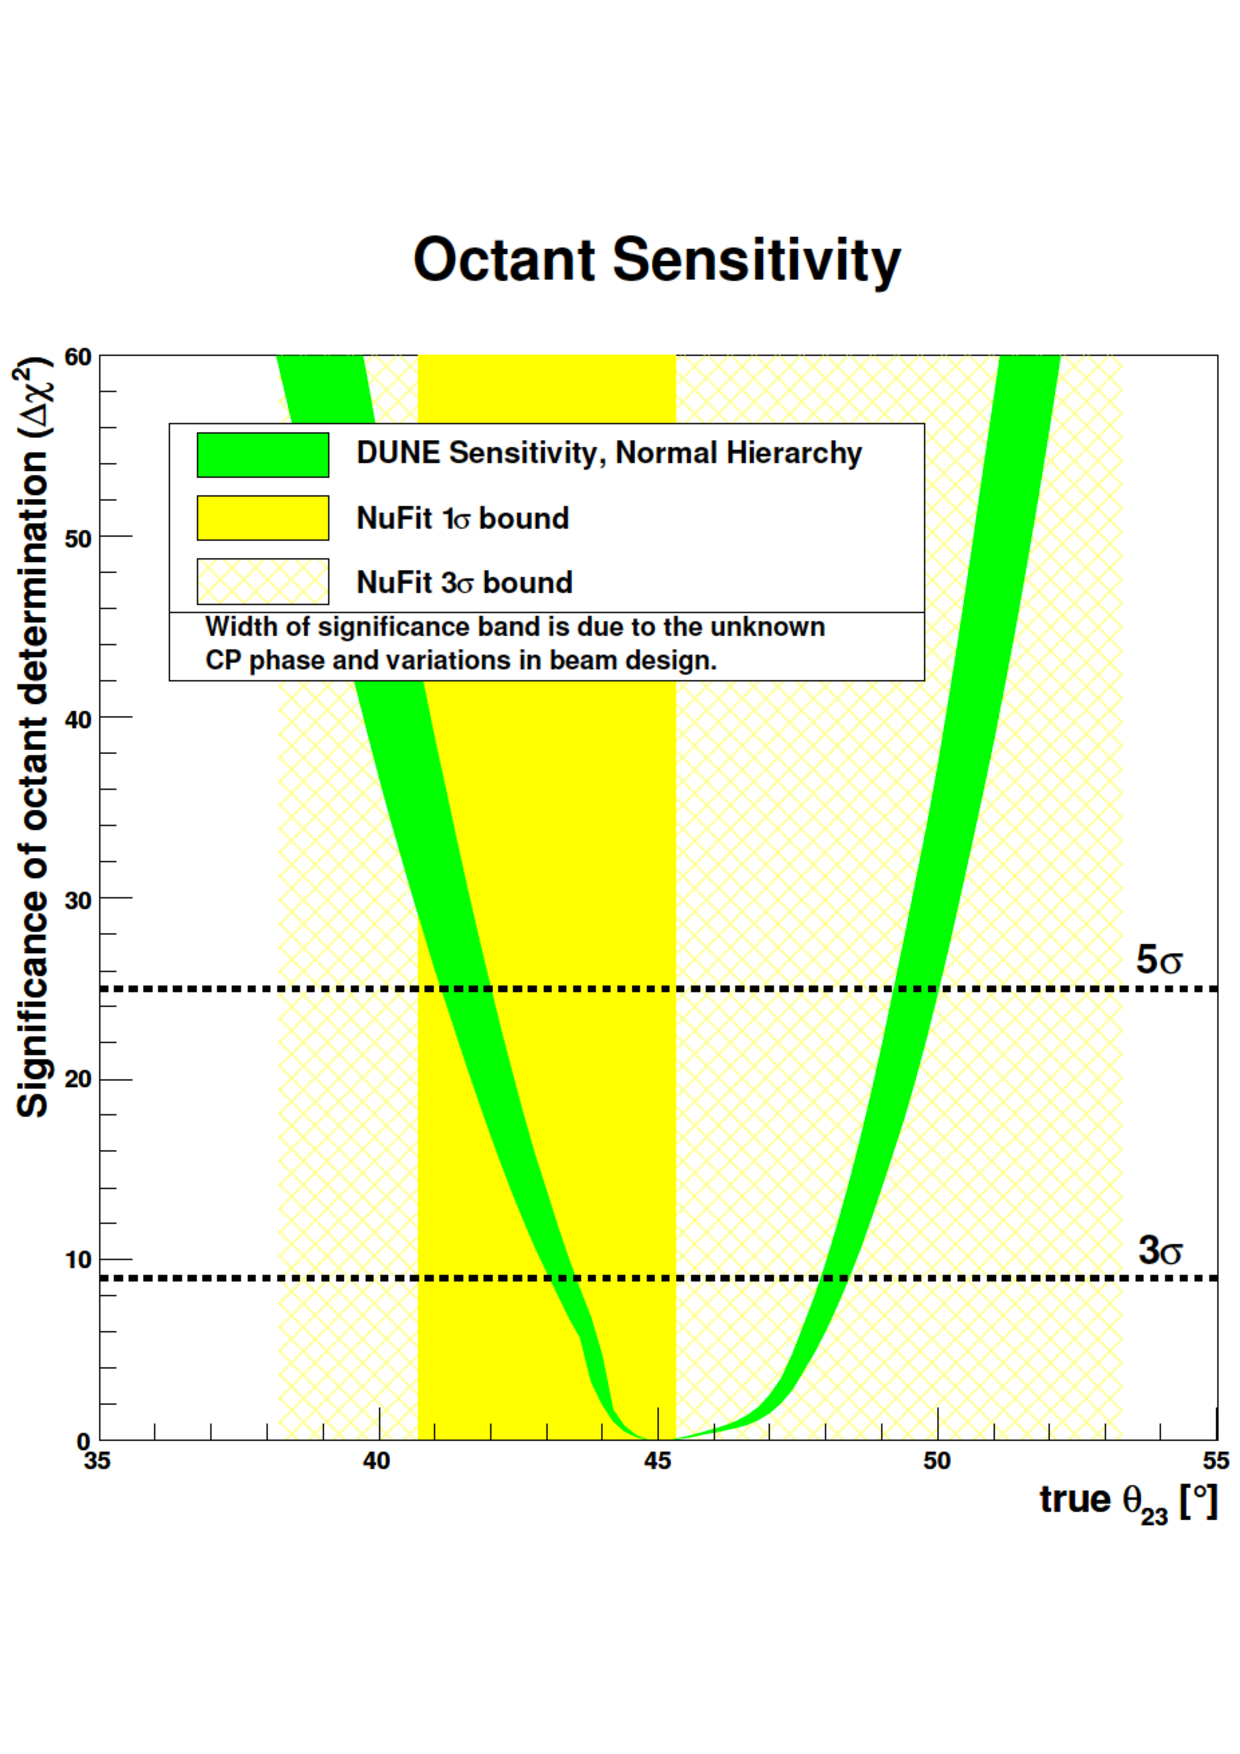
\includegraphics[width=0.5\textwidth]{DUNEOctantDetermination}
  \caption[The significance to which the octant of $\theta_{23}$ can be determined, for different values of $\theta_{23}$]
          {The significance to which the octant of $\theta_{23}$ can be determined, for different values of $\theta_{23}$. A beam exposure of 800~kt$\cdot$MW$\cdot$years is assumed, offering a 3$\sigma$ determination of the value of $\delta_{CP}$ for 75\% of the values of $\delta_{CP}$. The green band shows the effect of \textcolor{red}{different potential beam designs, and variations in the true value of $\delta_{CP}$}~\citep{DUNECDR_V3}. The yellow regions show the 1$\sigma$ and 3$\sigma$ bands. The figure is taken from~\citep{DUNECDR_V2}.}
  \label{fig:DUNEOctantDetermination}
\end{figure}

\begin{figure}
  \centering
  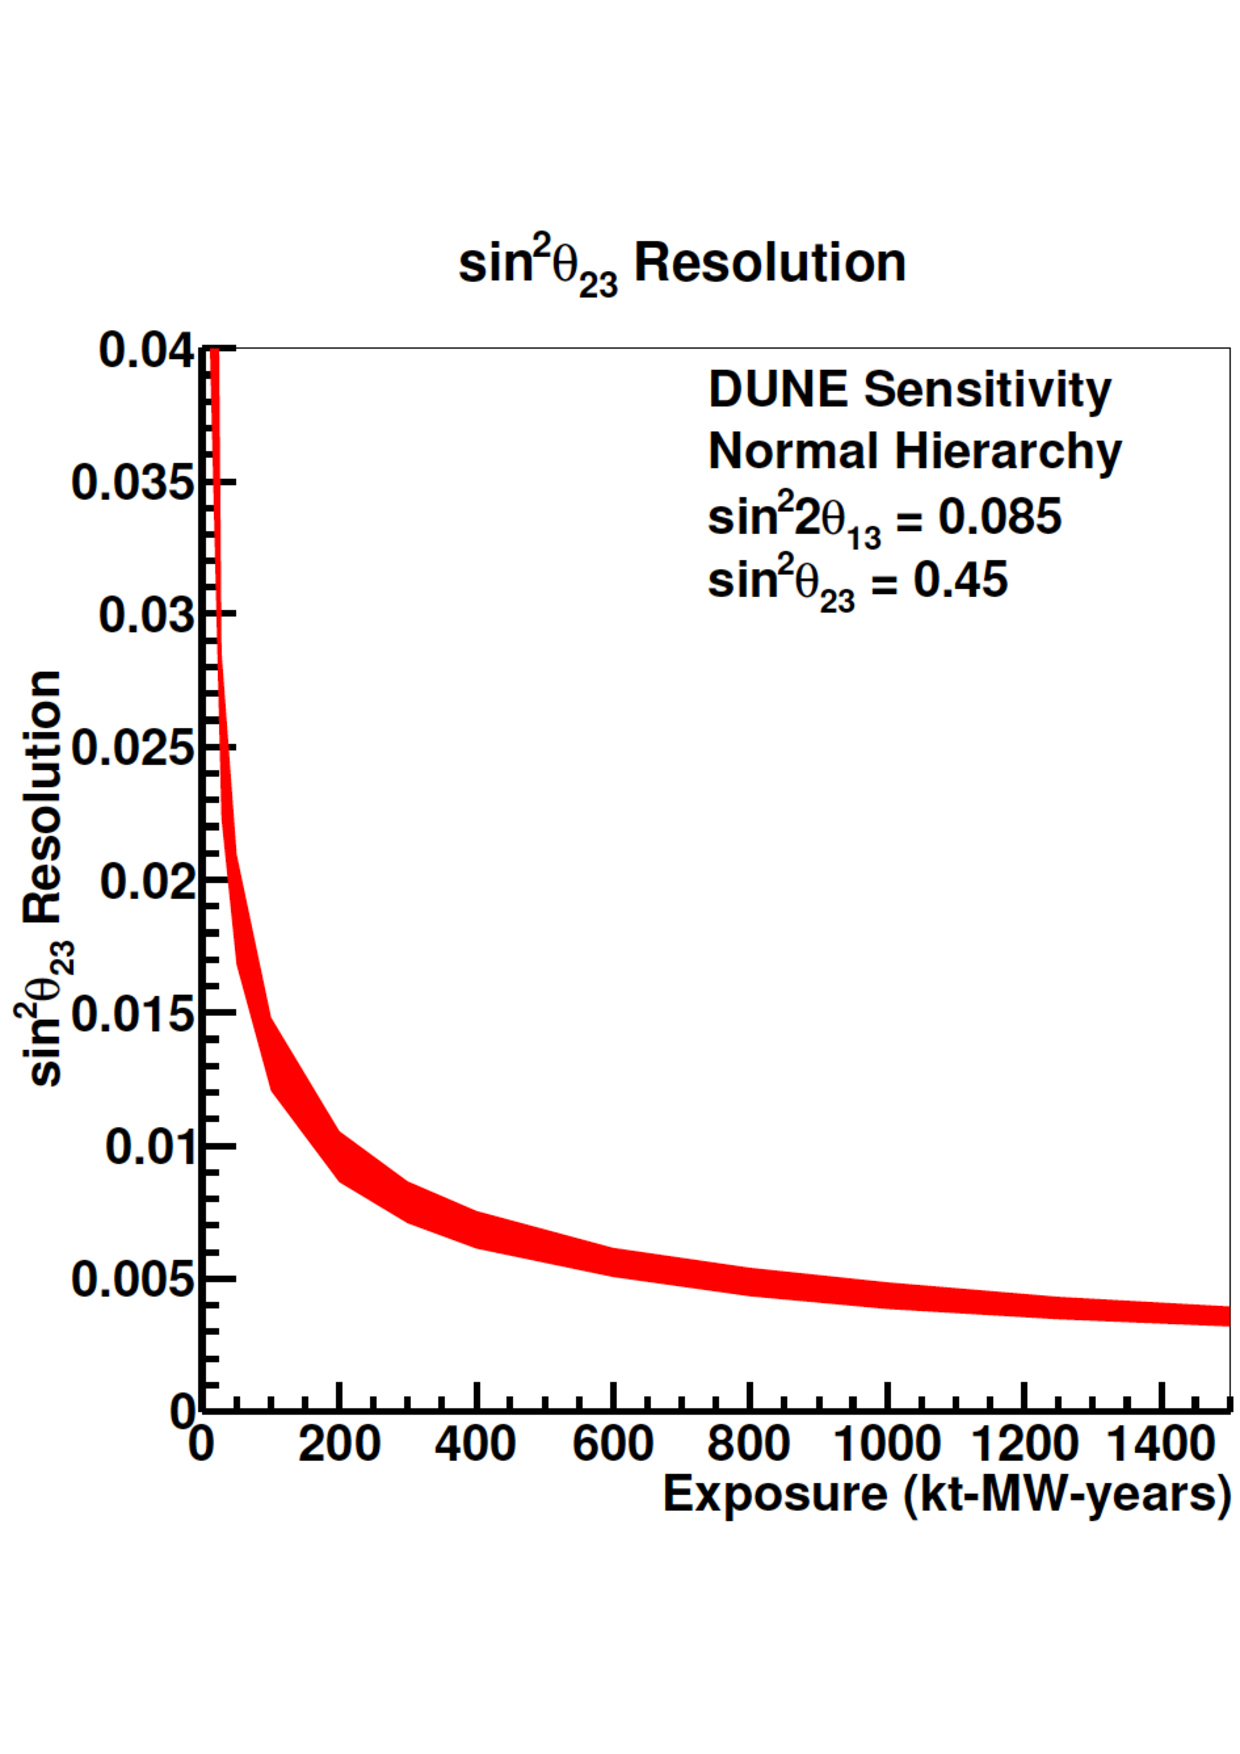
\includegraphics[width=0.5\textwidth]{DUNETheta23Res}
  \caption[The resolution with which DUNE will be able to determine the value of $\sin^{2}\theta_{23}$ for increasing beam exposures]
          {The resolution with which DUNE will be able to determine the value of $\sin^{2}\theta_{23}$ for increasing beam exposures. A normal hierarchy is assumed, and the band shows the \textcolor{red}{range of senstivities given variations in the potential beam design}~\citep{DUNECDR_V3}. The values for $\sin^{2}2\theta_{13}$ and $\sin^{2}\theta_{23}$ are the current best fit values from~\citep{NuFit2014}. The figure is taken from~\citep{DUNECDR_V2}.}
  \label{fig:DUNETheta23Res}
\end{figure}

The precision with which the values for $\sin^{2}\theta_{13}$ and $\Delta m^{2}_{31}$ can be measured by DUNE, are shown in Figure~\ref{fig:DUNETheta13Res} and Figure~\ref{fig:DUNEDeltaMRes} respectively. The resolution to which DUNE can measure the value of $\sin^{2}\theta_{13}$ is unlikely to surpass that of reactor experiments. However, DUNE will measure $\sin^{2}\theta_{13}$ using $\nu_e$ and $\overline{\nu_e}$ appearance, as opposed to $\overline{\nu_e}$ disappearance, as is done in reactor experiments. This complementary measurement of $\sin^{2}\theta_{13}$ will provide an independent constraint on the three-flavour mixing matrix. DUNE will also be able to greatly improve the resolution to which the $\Delta m^{2}_{31}$ mass splitting can be determined~\citep{DUNECDR_V2}. \\

\begin{figure}
  \centering
  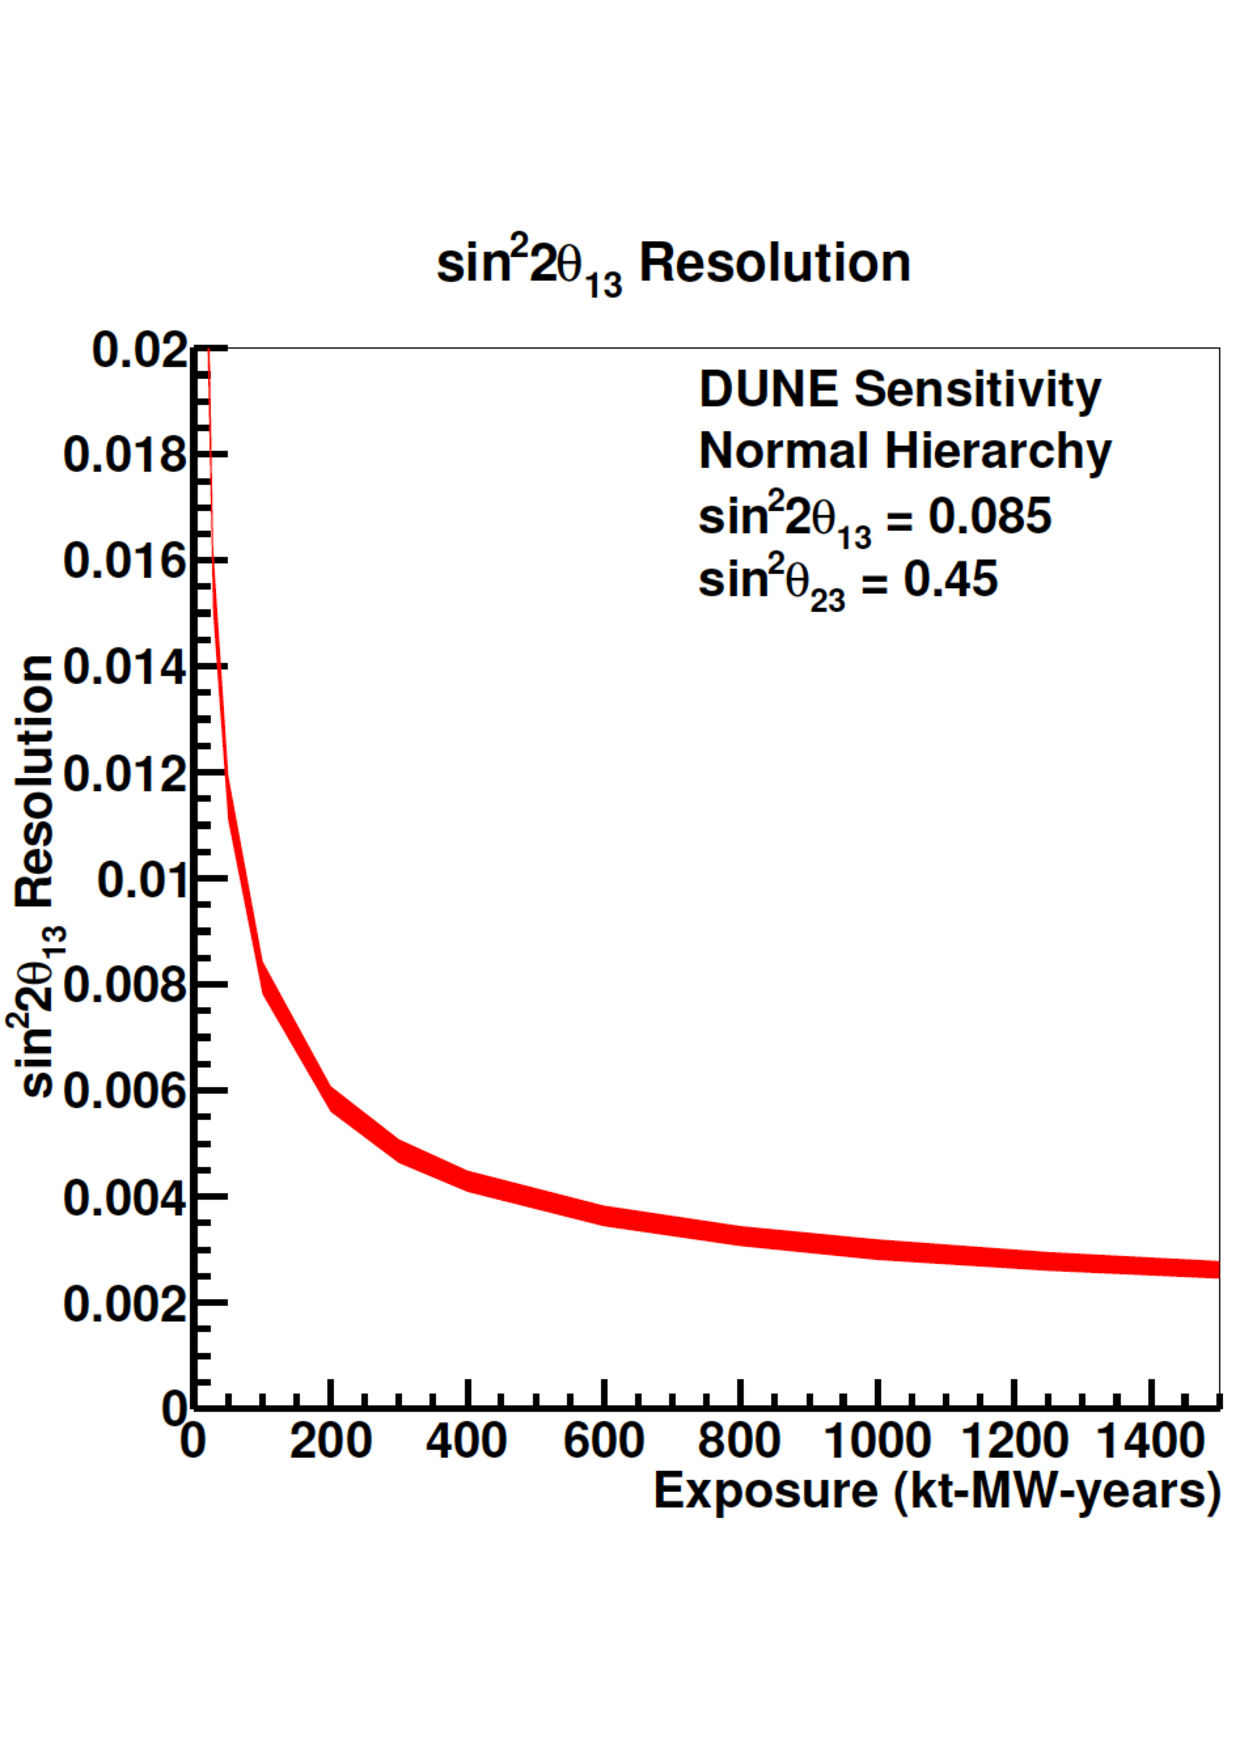
\includegraphics[width=0.5\textwidth]{DUNETheta13Res}
  \caption[The resolution with which DUNE will be able to determine the value of $\sin^{2}\theta_{13}$ for increasing beam exposures]
          {The resolution with which DUNE will be able to determine the value of $\sin^{2}\theta_{13}$ for increasing beam exposures. A normal hierarchy is assumed, and the band shows the \textcolor{red}{range of senstivities given variations in the potential beam design}~\citep{DUNECDR_V3}. The values for $\sin^{2}2\theta_{13}$ and $\sin^{2}\theta_{23}$ are the current best fit values taken from~\citep{NuFit2014}. The figure is taken from~\citep{DUNECDR_V2}.}
  \label{fig:DUNETheta13Res}
\end{figure}

\begin{figure}
  \centering
  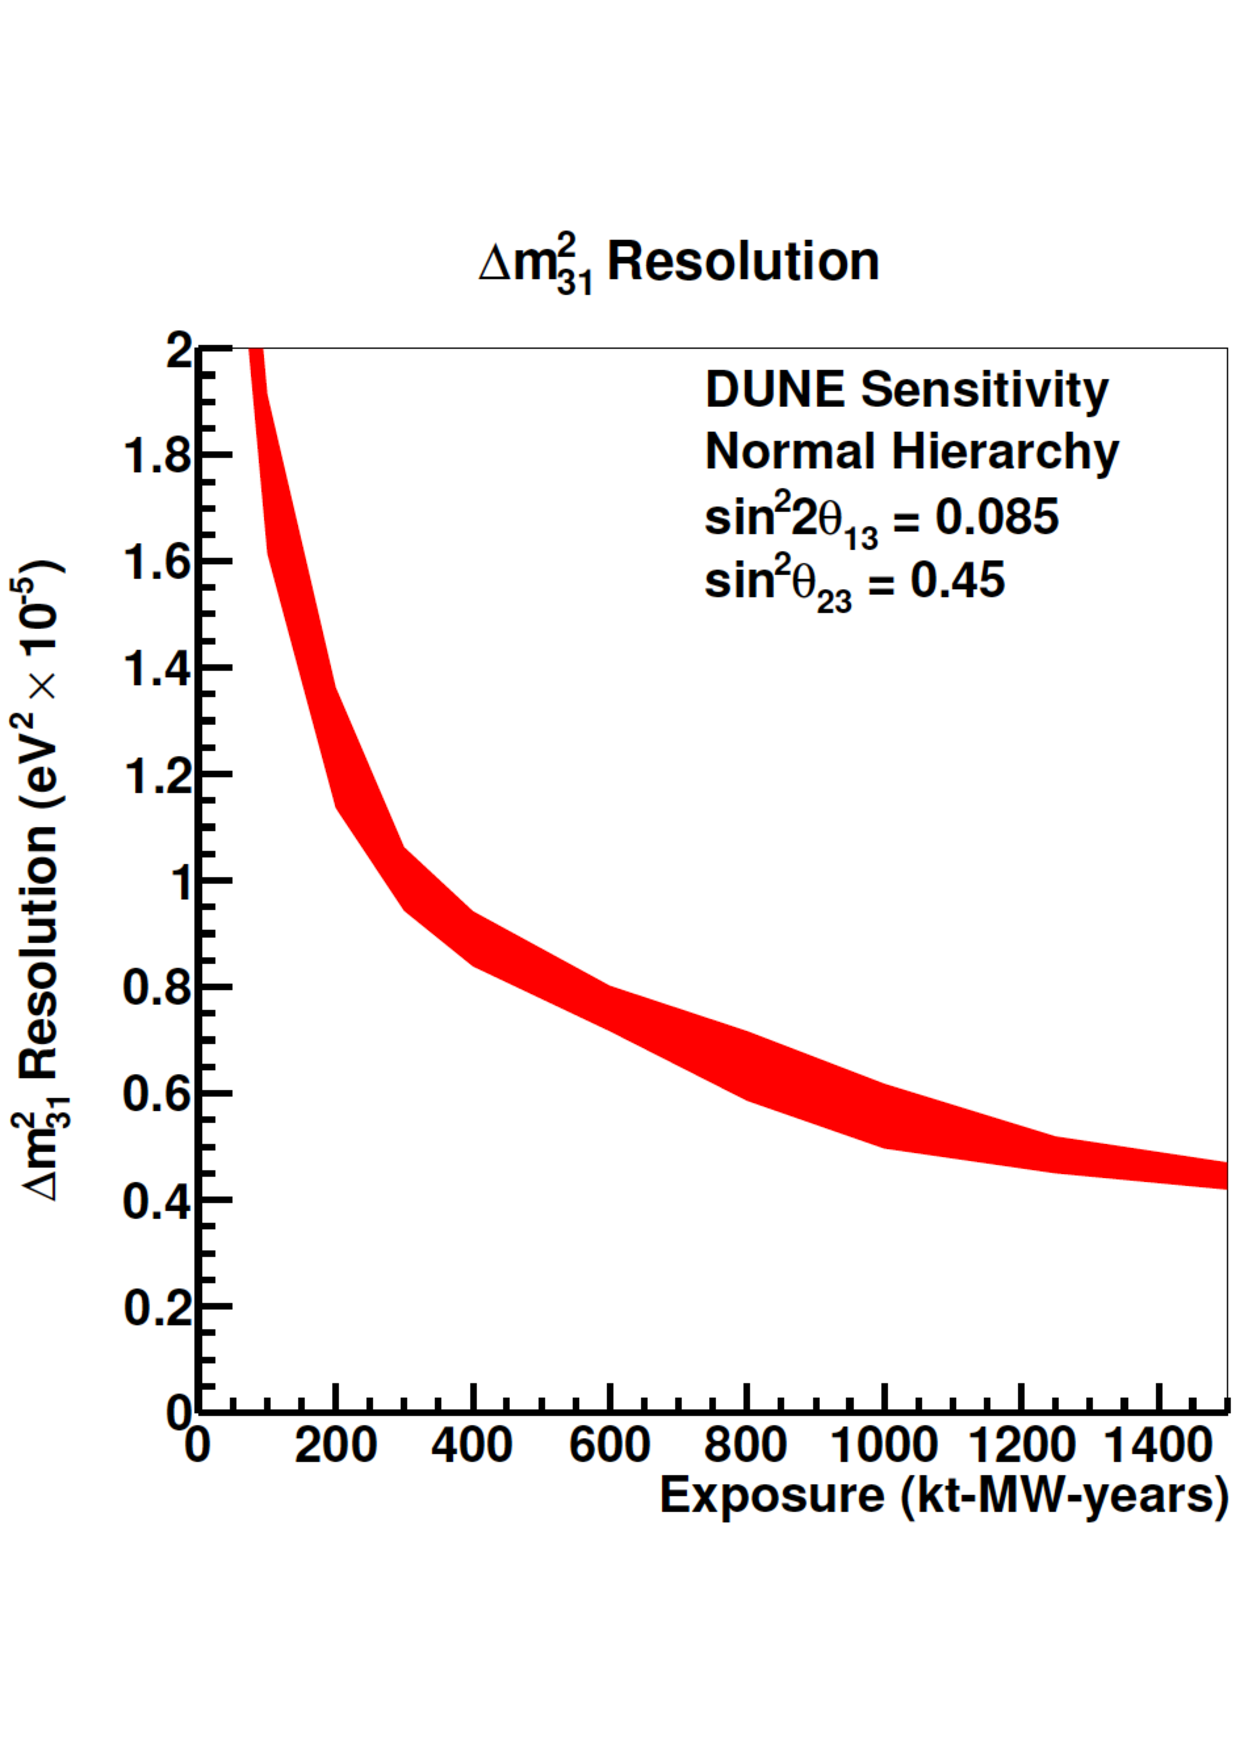
\includegraphics[width=0.5\textwidth]{DUNEDeltaMRes}
  \caption[The resolution with which DUNE will be able to determine the value of $\Delta m^{2}_{31}$ for increasing beam exposures]
          {The resolution with which DUNE will be able to determine the value of $\Delta m^{2}_{31}$ for increasing beam exposures. A normal hierarchy is assumed, and the band shows the \textcolor{red}{range of senstivities given variations in the potential beam design}~\citep{DUNECDR_V3}. The values for $\sin^{2}2\theta_{13}$ and $\sin^{2}\theta_{23}$ are the current best fit values taken from~\citep{NuFit2014}. The figure is taken from~\citep{DUNECDR_V2}.}
  \label{fig:DUNEDeltaMRes}
\end{figure}

It is also possible to measure many of the properties of neutrino mixing using atmospheric neutrinos. This is because atmospheric neutrinos contain all flavors of neutrinos and antineutrinos, and cover a wide range of $L/E$ values. Also, atmospheric neutrinos are always available. This is particularly useful because, as discussed in Section~\ref{sec:DUNEOverview}, the DUNE schedule has two of the four FD modules becoming operational before the beam is ready. As is the case in experiments such as Super-Kamiokande, DUNE can observe the differences in upwards and downwards going neutrinos. The enhanced detector resolution of LArTPCs allows DUNE to have a comparable sensitivity to the mass hierarchy as the proposed Hyper-Kamiokande experiment, despite having a much smaller fiducial mass~\citep{DUNECDR_V2}. \textcolor{red}{This can be seen in the plots shown in the most recent proposal for HK which involves placing a second detector in South Korea to take advantage of additional matter effects~\citep{Abe:2016ero}. From this paper it can be seen that after 20 years of running HK will have almost identical sensitivities to the resolution of $\delta_{CP}$ and the neutrino mass hierarchy as the figures shown above for DUNE.} 

%********************************** % 3.2 Section  *************************************
\subsection{Nucleon decay} \label{sec:DUNE_NDK}%Section - X.2.2
As presented in Section~\ref{sec:Theory_GUT}, many so called Grand Unified Theories (GUTs) predict some form of nucleon decay. Though nucleon decay has never been observed, it has not been completely ruled out. \textcolor{red}{Should a nucleon decay event be observed; it would appear as a roughly 1~GeV energy deposition in the detector which would ideally be isolated and fully contained. In reality, the observed energy would be less than this, as significant amounts of energy can be lost due to the production of neutral particles such as neutrinos which would not deposit energy in the detector.} As DUNE will be located deep underground, it will have a low background rate due to cosmic rays. This, combined with the high resolution of a LArTPC, means that DUNE offers a good opportunity to continue the search for nucleon decay. \\

Nucleon decay has been searched for by studying many decay channels, the current longest partial lifetime is in the $p \rightarrow e^{+} \pi^{0}$ decay channel. In this decay, the total mass of the proton should be converted into the electromagnetic showers produced by the two particles, and their net momentum should be zero. This is a signal which can be clearly identified in water Cherenkov detectors, such as Super-Kamiokande (SK), and so is the main decay mode which these detectors look for. This decay mode should also produce a clear signal in a LArTPC such as DUNE, though the limit that DUNE will place on this decay mode will not be competitive with that of Hyper-Kamiokande (HK), the successor to SK, due to the much smaller mass of DUNE. The $p \rightarrow K^{+} \overline{\nu}$ decay mode is particularly interesting in DUNE, as kaons should be able to be accurately identified in a LArTPC. This is not the case in a water Cherenkov detector, as the kaons are not energetic enough to produce Cherenkov light. This is true for all decay modes which have a kaon in the final state, including neutron decay modes. It is also important to note that DUNE will search for all types of baryon number non-conservation, including bound neutron decays, di-nucleon decay modes and neutron-antineutron oscillations. An analysis concerning the $n \rightarrow K^{+} + e^{-}$ decay channel will be presented in Section~\ref{sec:DUNENDK}. \\

It is hoped that DUNE will be able to reach sensitivities to nucleon decay lifetimes of between $10^{33}-10^{35}$~years. Figure~\ref{fig:DUNE_NDK_Lifetime} shows a comparison of current and potential lifetime limits for some decay modes, from a range of experiments. It can be seen that DUNE will provide very stringent limits to nucleon decay lifetimes, which will compete with HK in all decay modes containing kaons in the final state. Cherenkov detectors are able to perform relatively background free studies in the $p \rightarrow e^{+} \pi^{0}$ channel and, due to its much larger mass, HK will be able to achieve a limit which is superior to DUNE. In the other channels however, the excellent spatial resolution of LArTPCs allows DUNE to compete with, and in many cases improve on, any limit which could be set by HK. \\

\begin{figure}
  \centering
  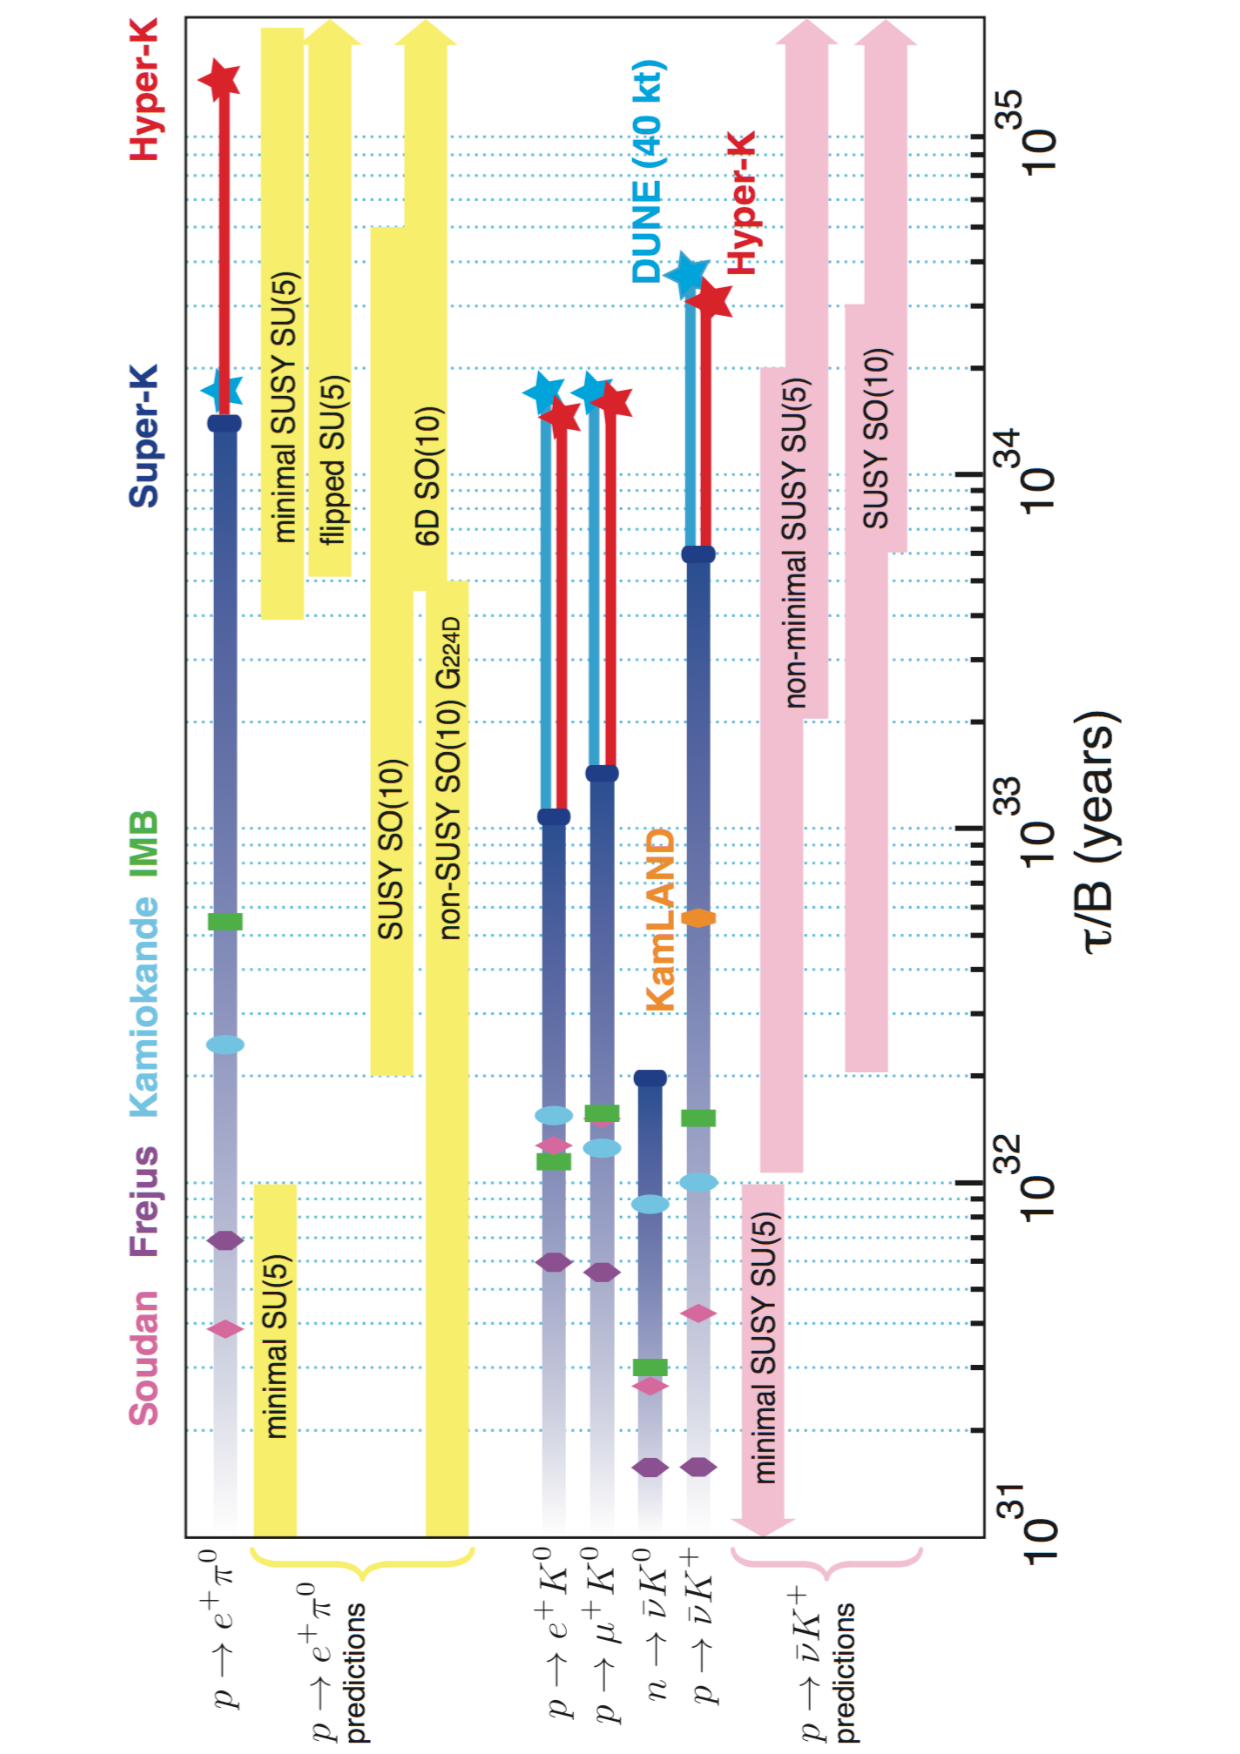
\includegraphics[width=0.8\textwidth]{NucleonDecayLimits}
  \caption[A comparison of current, and future, nucleon decay lifetime limits, compared with the ranges predicted by Grand Unified Theories.]
          {A comparison of current, and future, nucleon decay lifetime limits, compared with the ranges predicted by Grand Unified Theories. Coloured bars are shown for published limits by a number of experiments~\citep{PDG2012, Nishino:2012bnw}. Stars are shown for projected limits by future experiments, these limits are calculated using Poisson statistics, and include predicted background rates. The lifetimes predicted by different models are shown for the $p \rightarrow e^{+} \pi^{0}$ and $p \rightarrow K^{+} \overline{\nu}$, decay modes. The figure is taken from~\citep{DUNECDR_V2}.}
  \label{fig:DUNE_NDK_Lifetime}
\end{figure}

When estimating the expected sensitivity of DUNE to a range of nucleon decay modes, previous studies have been used~\citep{Bueno, Klinger:2015kva}. Some of the channels where one would expect a LArTPC, such as DUNE, to have an advantage in signal efficiency when compared to a water Cherenkov detector, such as SK/HK, are shown in Table~\ref{tab:NDKLim}. The accurate tracking of the kaon, and its subsequent decay products, is the reason for the increased signal efficiency that is expected in LArTPCs. The ability for LArTPCs to perform tracking to this accuracy was seen by the ICARUS collaboration, using the T600 detector~\citep{PMTrack}. Figure~\ref{fig:ICARUSKaon} shows an example event where a kaon enters the detector and is seen to decay to a muon, which subsequently decays to an electron. \\

\begin{table}
  \caption[Nucleon decay limits in DUNE and Super-Kamiokande, in some favoured decay channels]
          {Nucleon decay limits in DUNE and Super-Kamiokande, in some favoured decay channels. The \textcolor{red}{currently measured lifetime limits} (Curr. limit), the estimated DUNE reconstruction efficiencies (DUNE $\epsilon$), and the estimated DUNE lifetime limit in 2034 (DUNE limit) are shown. For comparison, the published Super-Kamiokande reconstruction efficiencies (SK $\epsilon$), and the estimated Super-Kamiokande lifetime limit in 2034 (SK limit) are also shown. All lifetimes shown, are partial lifetimes, in units of 10$^{33}$~years. The table is taken from~\citep{MauryLifetime}, which uses~\citep{PDGReview}.}
  \centering
  \label{tab:NDKLim}
  %\scriptsize
  \begin{tabular}{l c c c c c}
    \toprule
    {Decay mode}                               & {Curr. limit} & {DUNE $\epsilon$ (\%)} & {DUNE limit} & {SK $\epsilon$ (\%)} & {SK limit} \\ 
    \midrule
    $p \rightarrow e^{+} \pi^{0}$              & 16.7          & 45.3              & 21.4         & 54              & 50.8       \\
    
    $p \rightarrow \pi^{+} \overline{\nu_{e}}$ & 0.016         & 41.9              & 19.8         & 54              & N/A        \\
    
    $p \rightarrow K^{+} \overline{\nu_{e}}$   & 0.051         & 97.0              & 29.7         & 11              & 2.1        \\
    
    $p \rightarrow \mu^{+} \pi^{0}$            & 7.78          & 44.8              & 21.1         & 54              & 50.8       \\
    
    $p \rightarrow K^{0} \mu^{+}$              & 1.6           & 46.7              & 22.0         & 100             & 22.2       \\

    $p \rightarrow K^{+} \pi^{+} e^{-}$        & 0.075         & 41.8              & 19.7         & 46              & 2.3        \\
    
    $n \rightarrow \pi^{0} \overline{\nu_{e}}$ & 0.112         & 45.1              & 26.0         & 30              & 7.1        \\
    
    $n \rightarrow K^{+} e^{-}$                & 0.032         & 96                & 55.4         & 100             & 1.8        \\
    \bottomrule
  \end{tabular}
\end{table}

\begin{figure}
    \centering
  \begin{subfigure}{0.48\textwidth}
    \centering
    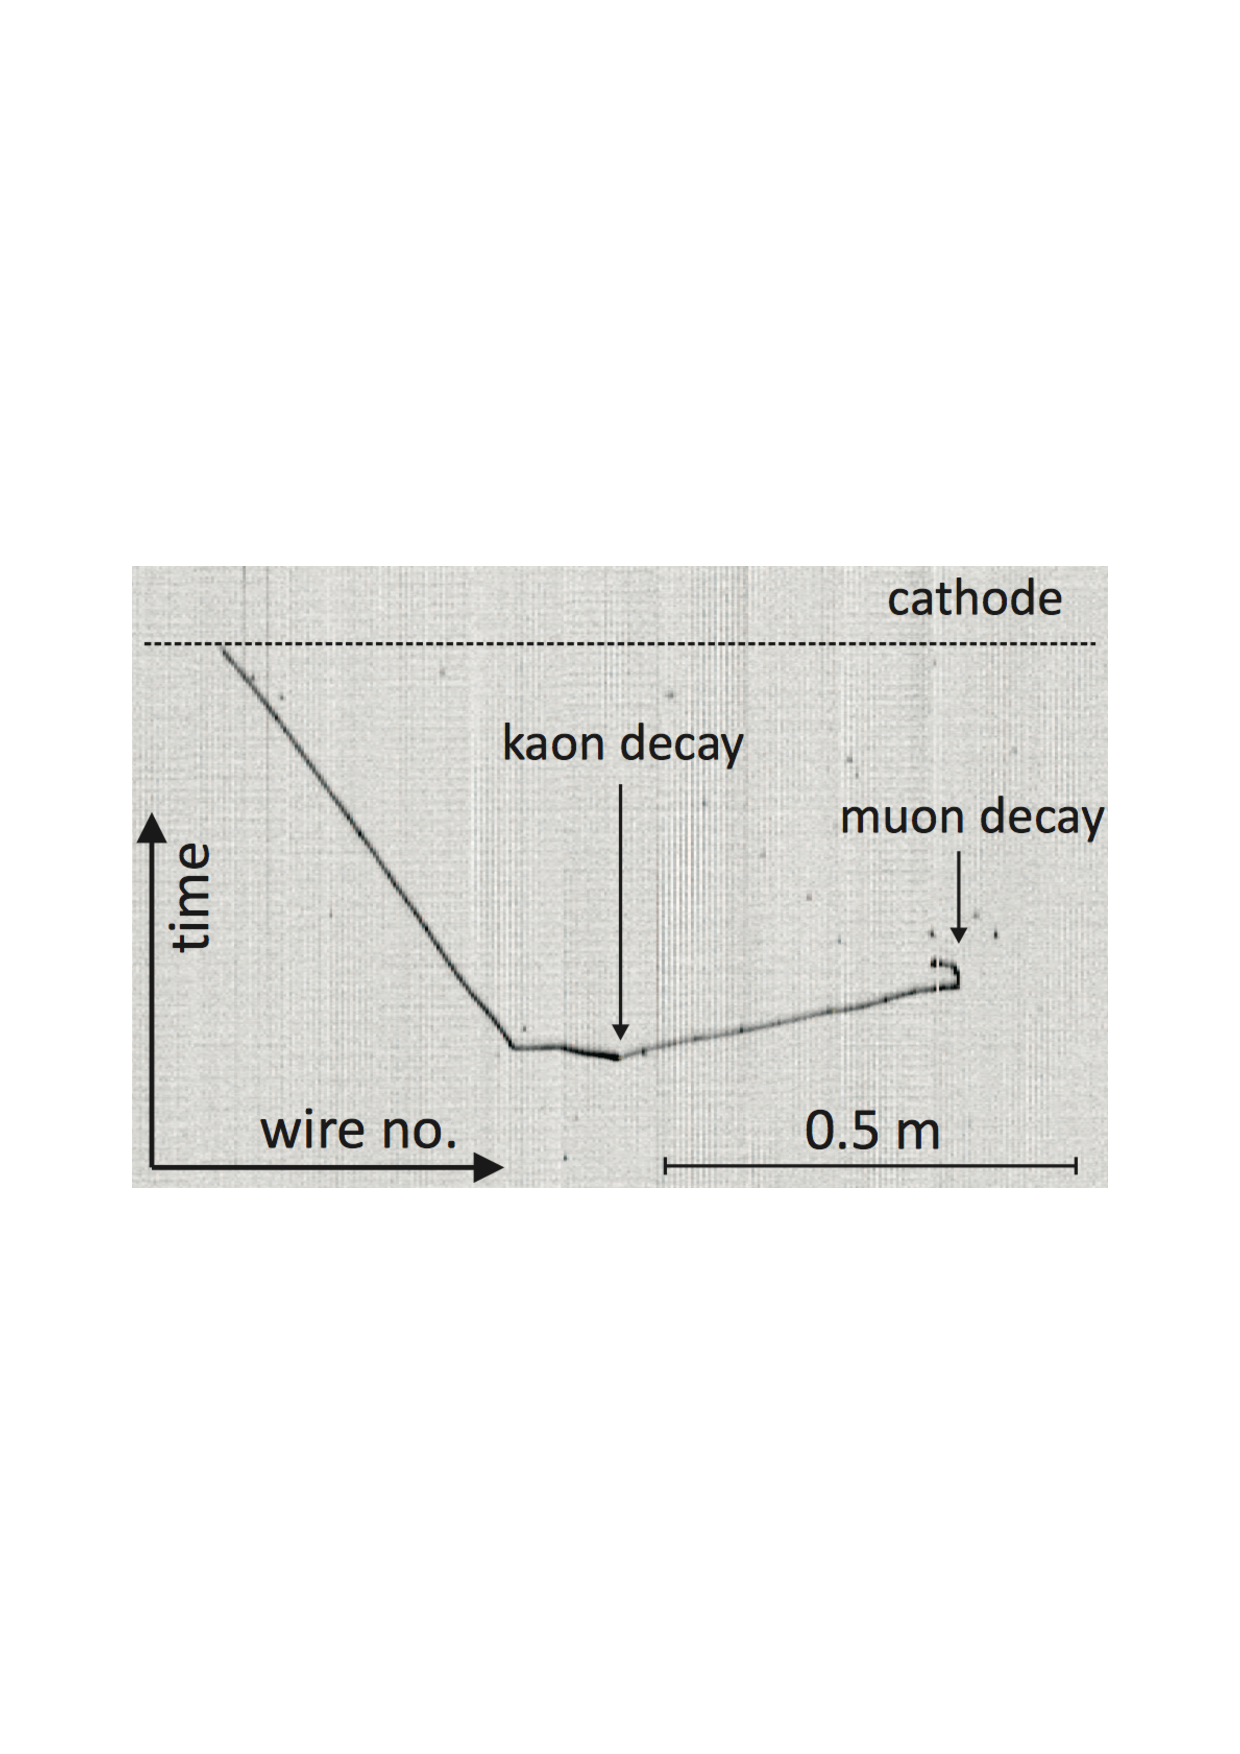
\includegraphics[width=\textwidth]{ICARUSKaon_Col}
    \caption{The collection plane view.}
  \end{subfigure}%
  \hspace{0.05\textwidth}
  \begin{subfigure}{0.42\textwidth}
    \centering
    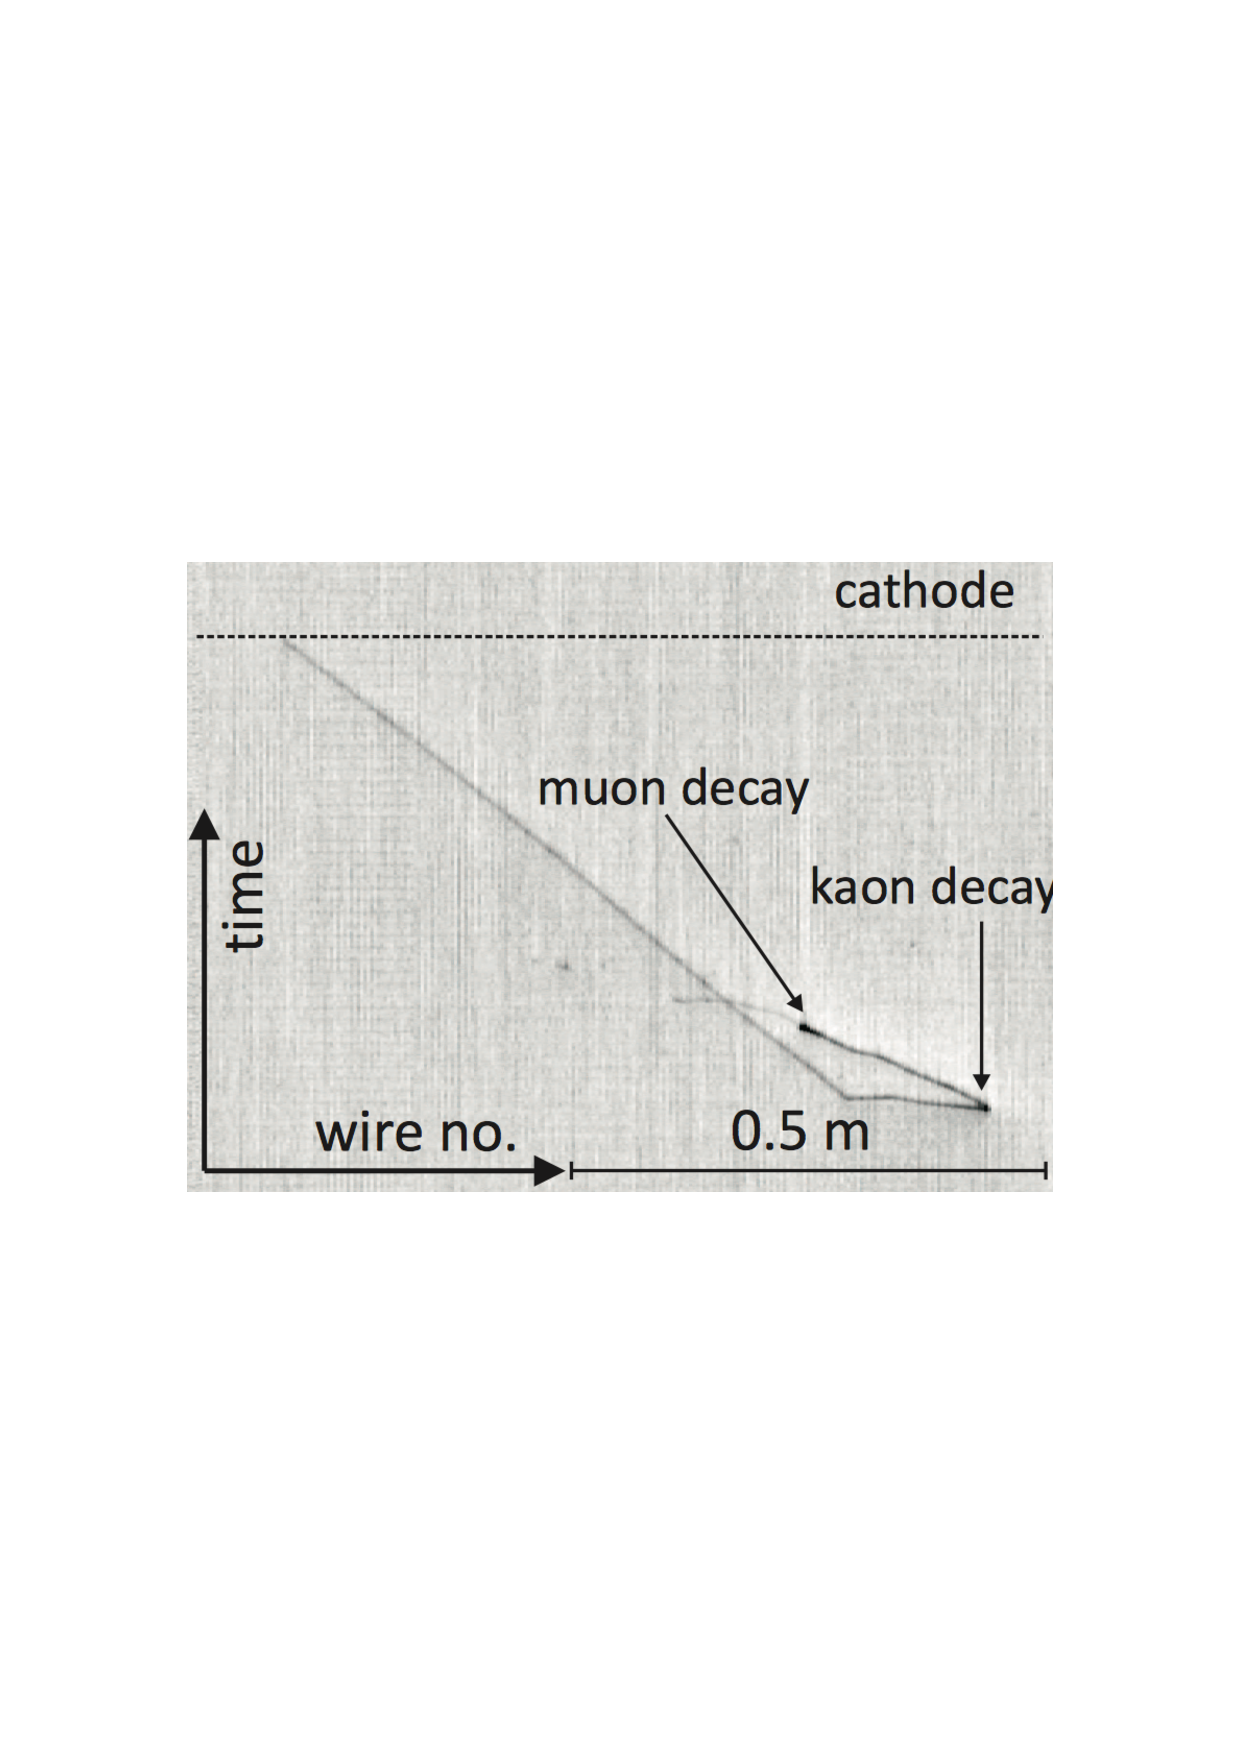
\includegraphics[width=\textwidth]{ICARUSKaon_Ind}
    \caption{The second induction plane view.}
  \end{subfigure}
  \caption[A kaon event which was observed in the ICARUS T600 detector, in the CNGS data]
          {A kaon event which was observed in the ICARUS T600 detector, in the CNGS data. Left: the signal on the collection plane. Right: the signal on the second induction plane. The kaon enters the detector and decays via $K \rightarrow \mu \nu$, the muon then decays via $\mu \rightarrow e \nu$. The figure is taken from~\citep{PMTrack}.}
  \label{fig:ICARUSKaon}
\end{figure}

Preliminary studies, at the time of writing the DUNE CDR documents, showed that after considering the backgrounds due to cosmic rays at depth, the backgrounds due to atmospheric neutrinos, and the impact of reconstruction failures, the number of background events for the $p \rightarrow K^{+} \overline{\nu_{e}}$ decay mode should be less than 1~event$\cdot$Mt$^{-1}\cdot$year~\citep{Klinger:2015kva, Adams:2013qkq, LBNE8836}. With a background rate this low, the observation of a single, well reconstructed event, could provide evidence of nucleon decay~\citep{DUNECDR_V2}. 

\subsection{Additional physics opportunities} \label{sec:DUNE_Other}%Section - X.2.2
Many of the largest detectors in the world would hope to observe neutrinos from a core-collapse supernova, should one occur during their lifetimes. DUNE is one of these experiments, and will have particularly good sensitivity to the electron flavour supernova neutrinos. This means that it should be possible to get a large, clean, supernova $\nu_e$ signal from DUNE, which is not possible using water Cherenkov detectors~\citep{KScholSND, Laha:2013hva}. Models predict that the full DUNE FD should observe about 3,000 events from a supernova at a distance of 10~kpc. The neutrino interactions from a supernova would consist of short electron tracks, which were potentially accompanied by a few gamma rays. \textcolor{red}{The energy threshold for observation of these supernova neutrinos is still being studied, but it is thought that the threshold will be a few 10's of MeV~\citep{DUNECDR_V2}.} The observation of a core-collapse supernova during the lifetime of DUNE could help answer some of the open questions which still remain after the observation of SN1987A~\citep{PhysRevLett.58.1494, PhysRevLett.58.1490}. \\
%The observation of a supernova within the Milky Way would allow a large suite of topics to be analysed. These include, but are by no means limited to: measurements of the neutrino mass splittings, measurements of the neutrino mixing parameters, measurements of neutrino ``self-refraction'' (possible due to the high density of neutrinos around the supernova), tests of Lorentz and CPT invariance, and of course testing all aspects of the predictions made my models of supernova~\citep{DUNECDR_V2}. \\

There are also other physics aspects which DUNE could make progress in, such as the indirect searches for WIMPs. This is because, should a flux of high energy neutrinos be observed to originate from the Sun, it could support the idea of dark matter annihilation. Searches for these interactions have been performed by IceCube~\citep{Aartsen:2012kia, Choi:2015ara}, but have not observed any signals. It is hoped that with the increased angular resolution of LArTPCs, the number of background events could be substantially reduced~\citep{DUNECDR_V2}. Other aspects where DUNE could make contributions are in searches for the diffuse supernova neutrino background~\citep{Beacom:2010kk}, searches for neutrinos from accretion disks~\citep{Caballero:2011dw}, and searches for black hole-neutron stars mergers~\citep{Caballero:2009ww}. \\

Hence, there is a very compelling case for building a LArTPC with a fiducial \textcolor{red}{mass} of approximately 40~kt, at a large depth underground. \\

%********************************** % Fourth Section  *************************************
\section{Path to building DUNE - The 35 ton prototype} \label{sec:The35tonDetector}  %Section - X.4
The DUNE FD modules represent an increase in size by more than an order of magnitude, when compared to existing LArTPCs. It is therefore necessary to build a robust prototyping schedule, a brief outline of which is shown in Figure~\ref{fig:DUNEProtSched}. It should be noted that DUNE will draw on the experience of all LArTPC experiments (MicroBooNE, SBND and many others), and so experiments not associated with DUNE will help shape the experiment through the improvements which they make to LArTPC technology. \\ 

\begin{figure}
  \centering
  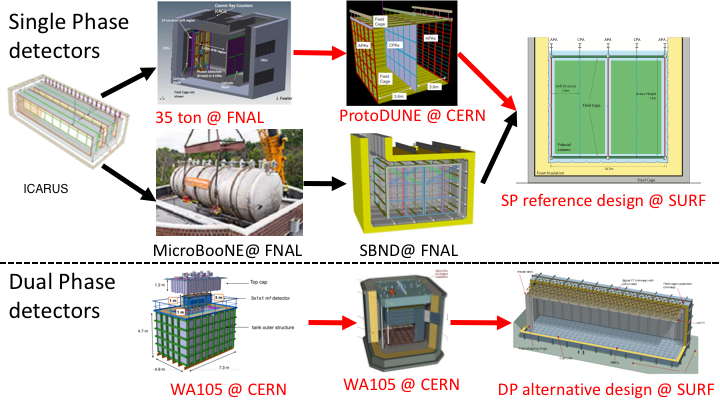
\includegraphics[width=0.98\textwidth]{PrototypeSched}
  \caption[An overview of the DUNE prototyping schedule, including complementary experiments]
          {An overview of the DUNE prototyping schedule, including complementary experiments. Top shows the experiments which utilise single phase LArTPC designs, whilst bottom shows experiments which utilise a two phase design. The experiments which are part of the DUNE prototyping program are shown in red. The figures are taken from~\citep{DUNECDR_V4, MarkReviewJuly2015}.}
  \label{fig:DUNEProtSched}
\end{figure}

The 35 ton detector is the first prototype under the umbrella of the DUNE experiment, for the single phase detector design. As such, the 35 ton detector provides a test bed for many of the novel aspects of the detector design required for the DUNE FD. This testing was done during two running periods, the Phase 1 run from November 2013 - February 2014, and the Phase 2 run from November 2015 - March 2016. Chapters~\ref{chap:Cameras},~\ref{chap:35tonSim}, and~\ref{chap:35tonData}, will focus on some of the studies performed in preparation for, and during, the Phase 2 run. \\ 

The primary goal of the Phase 1 run was to verify that a detector with a membrane cryostat could achieve, and maintain, the high levels of LAr purity which are required to perform the physics which DUNE is expected to achieve. It was also designed to show that it was possible to achieve this high level of purity without the need to fully evacuate the detector prior to filling, but that this could instead be achieved by performing a ``piston purge.'' This ``piston purge'' had previously been demonstrated by the Liquid Argon Purity Demonstrator (LAPD)~\citep{LAPD}, which the 35 ton was built next to, at Fermilab's PC-4 facility. The process by which the ``piston purge'' was performed is as follows. Firstly, room temperature argon is pumped into the detector, displacing the air in the detector. Once the purity is no longer seen to improve, a gas/liquid spray is used to slowly cool the detector. The injection of the spray introduces turbulence into the gas in the detector, which causes the entire cryostat to cool, avoiding large temperature differences. Upon the completion of the cooldown, filling of the LAr commences, and LAr purification is performed using the installed recirculation loop. Using this purification method, electron lifetimes of 3 ms were observed after a few days of purification. These purity levels were maintained for many days at a time, thus demonstrating that membrane cryostat technology is capable of producing, and maintaining, high purity LAr~\citep{35tonMontanari, 35tonHahn}. \\

A detector similar to ProtoDUNE (outlined below), was originally planned to follow the Phase I run. However, funding constraints meant that this detector (at the time part of LBNE) got cancelled, and so the 35 ton cryostat was repurposed to contain a number of TPCs. This repurposed detector is the 35 ton Phase II run. The installed TPCs were designed to have many of the features which are present in the single phase reference design, these include:
\begin{itemize}
\item Modular APAs with wrapped wires, collecting charge \textcolor{red}{from} multiple drift volumes.
\item Vertical and horizontal gaps between APAs. The Phase II run must show that it is possible to stitch particle tracks across, and through, APA frames.
\item APAs and electronics which are immersed in the LAr.
\item Waveguide-style photon detectors, installed inside the APA frames.
\item A field cage built using printed circuit board.
\item A DAQ which is capable of triggerless operation.
\end{itemize}
All of these features are central to the single phase DUNE detector design, and so demonstrating the successful operation of a detector with these properties is an important step in realising DUNE. Getting the Liquid Argon Software (LArSoft) framework (outlined in Section~\ref{sec:LArSoft}) ready for data taking required extensive simulation work, some of which is presented in Chapter~\ref{chap:35tonSim}. \\

In total four APAs were installed in the 35 ton cryostat, each collecting charge from two drift volumes, to give a total of 8 TPCs. As the total drift volume for the 35 ton was spatially limited to around 2.5 m, it was not possible to use TPCs with the drift length which will be present in the DUNE FD design. As such, it was decided that the TPCs would either have a ``long'' drift volume of 2.23 m, or a ``short'' drift volume of 0.27 m. These lengths were chosen so as to represent a reasonable drift distance in the ``short'' drift volume, whilst also maximising the ``long'' drift distance. Of the four APAs which were installed, two were ``tall'', and were 120~cm in height, whilst the other two APAs were ``short'', being 60~cm in height, and were stacked on top of each other, sandwiched between the two ``tall'' APAs. All of the APAs were 30~cm wide. This orientation allowed both vertical, and horizontal gaps to be produced, over which the reconstruction algorithms could attempt to stitch tracks. A total of 8 photon detectors were installed in the APAs, with 3 PDs in each of the ``tall'' APAs, and 1 PD in each of the ``short'' APAs. Figure~\ref{fig:35tonSchem} shows a schematic of the 35 ton detector. \\

\begin{figure}
  \centering
  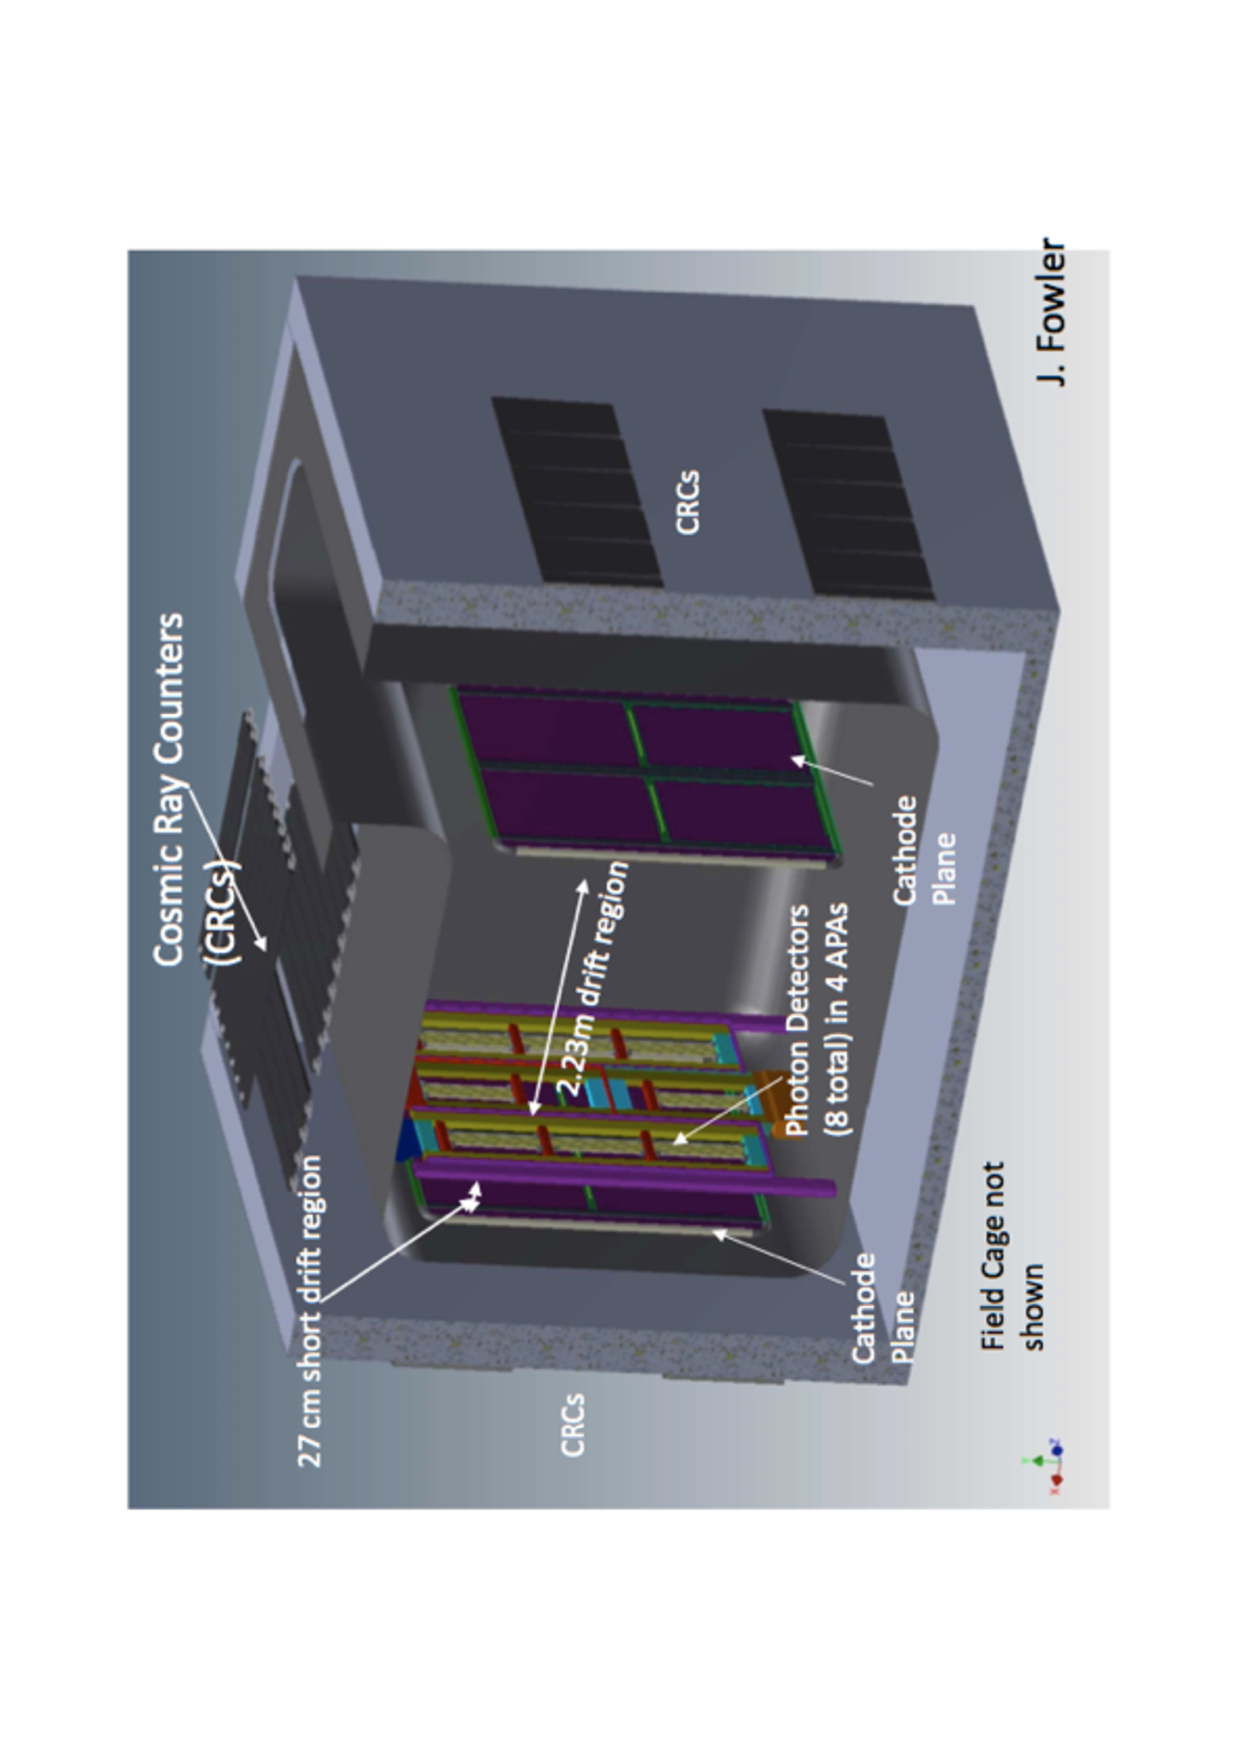
\includegraphics[width=0.85\textwidth]{35tonSchem}
  \caption[A schematic representation of the 35 ton prototype detector during the Phase II run]
          {A schematic representation of the 35 ton prototype detector during the Phase II run. The cathode planes (dark purple), photon detectors (yellow), APA frames (bounded light purple regions), cosmic rays counters (outer black rectangles), and the two drift volumes (2.23 m and 0.27 m) are shown. The photon detectors are in the middle of the APA frames, with the wire planes being on the outside of the APA frames. The 35 ton vessel (spotted grey), and steel container (black) are also shown. The field cage is not shown. Cryogenic piping for the detector is placed within the cryostat, to the right of the cathode plane associated with the ``long'' drift. The figure is taken from~\citep{DUNECDR_V4}.}
  \label{fig:35tonSchem}
\end{figure}

A system of Cosmic Ray Counters (CRCs) can be seen on the outer edges of the cryostat walls in Figure~\ref{fig:35tonSchem}. These were installed so that sets of cosmic muons could be recorded which were either parallel, or perpendicular, to the APA frames, as it was envisioned that these muons would be useful for later studies. There was also an additional set of CRCs on top of the cryostat to collect muons which were nearly vertical. The location of the 35 ton was not in a beamline, because, as discussed earlier, it was not originally intended to house TPCs. As such, only cosmic ray data was collected in the Phase II run, and so the muons identified by these CRCs produced a very valuable subset of the data, as will be seen in Chapter~\ref{chap:35tonData}. The locations, and numbering scheme for the CRCs, is shown in Figure~\ref{fig:35tonCounterLoc}, and will be used extensively in Chapter~\ref{chap:35tonData}. \\

\begin{figure}
  \centering
  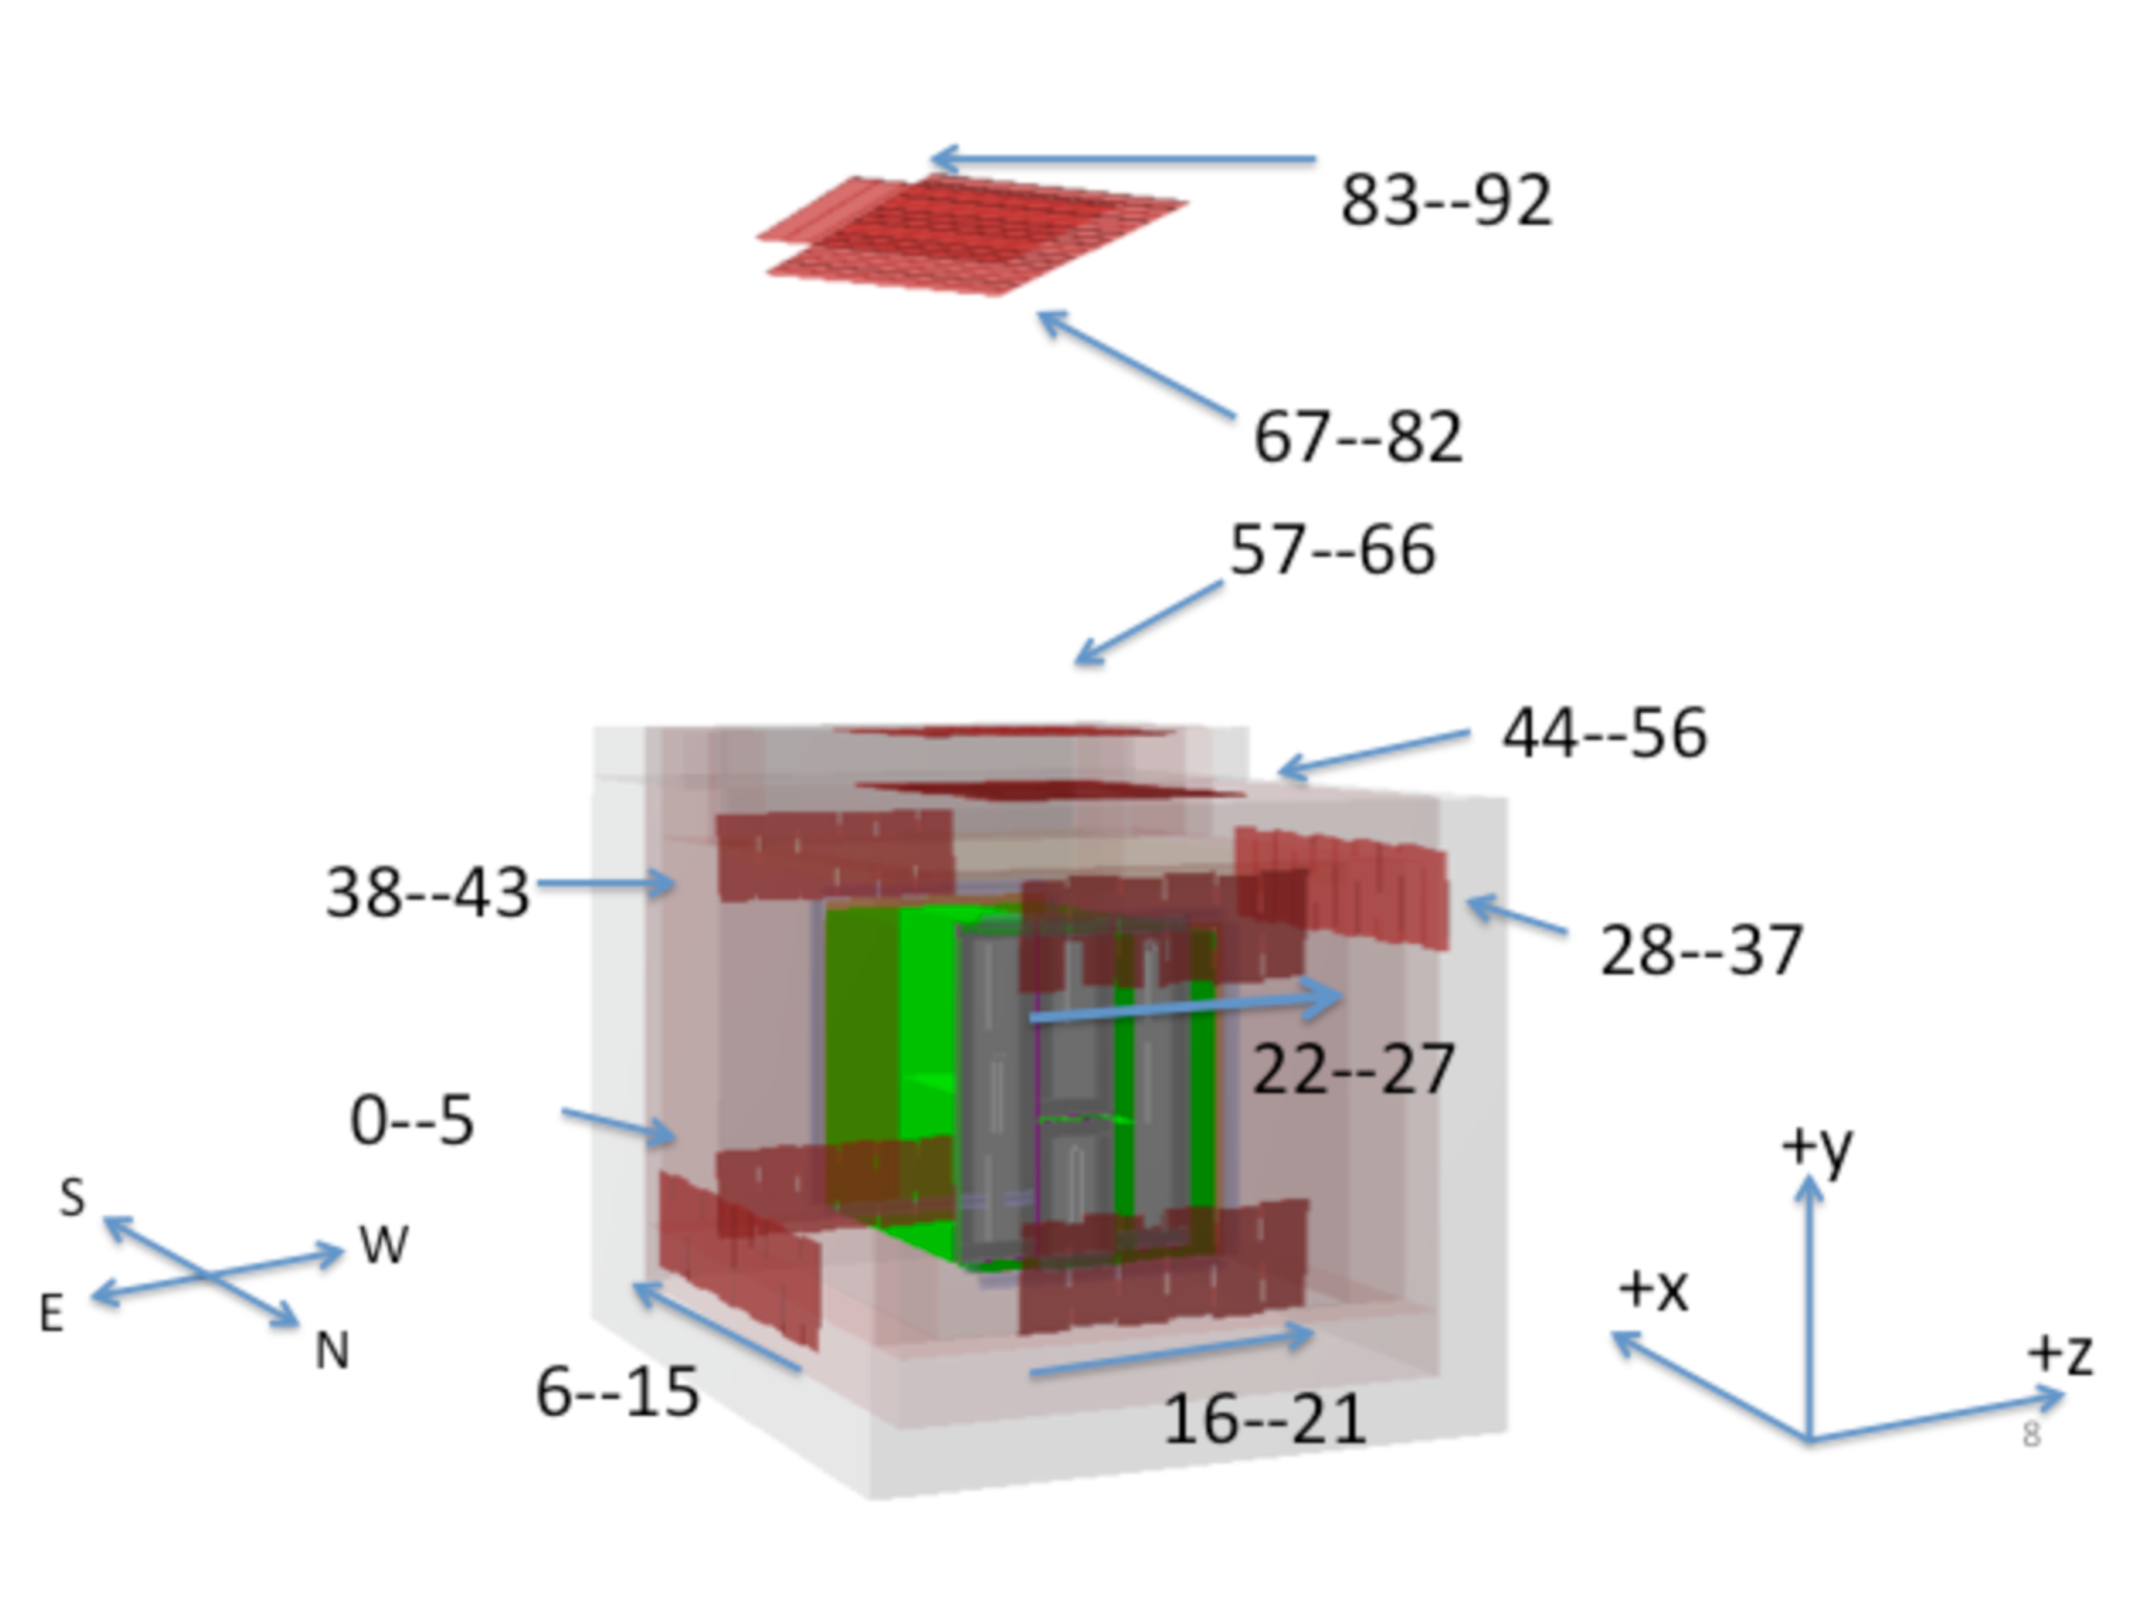
\includegraphics[width=0.85\textwidth]{35tonFullDetect}
  \caption[A representation of the cosmic ray counter locations in the 35 ton]
          {A representation of the cosmic ray counter locations in the 35 ton, with the geographic, and LArSoft, coordinate systems shown. The other detector components can be seen inside the cryostat, such that the cosmic ray counters on the north wall are behind the short drift volume. The east~-~west counters are numbered 6-15 and 28-37 respectively. The north~lower~-~south~upper counters are numbered 16-21 and 38-43 respectively. The north~upper~-~south~lower counters are numbered 22-27 and 0-5 respectively. The ``telescope'' (vertically through-going) counters are numbered 44-92 and are split into four groups.}
  \label{fig:35tonCounterLoc}
\end{figure}

The Phase II run built on the experience gained during the Phase I run, using the same process for the initial cooldown, and LAr recirculation. The run also served to show that the electron lifetime which could be achieved was not limited by the presence of an instrumented detector. The operation of the installed TPC also served to test many of the novel features of the FD reference design. Some of the results from the Phase II run are shown in Chapter~\ref{chap:35tonData}. \\

Following on from the 35 ton Phase II run, the single phase ProtoDUNE detector is under construction at CERN, and is due to take data in the second half of 2018. The ProtoDUNE detector is a small version of the full DUNE single phase reference design, as the APAs, and the drift length, are the same size as those in the reference design. The detector will be in a charged particle test beam, and so will be able to fully test the assumptions made in the DUNE CDRs about the detector performance characteristics. The detector will contain two sets of three APAs, 7.2 m apart, with one set of CPAs between them. This will give a total of 6 TPCs, each with a drift length of 3.6 m. \\

There is also a series of prototypes for the two phase design. The WA105 project involves both a small scale demonstrator, with an active mass of 1~$\times$~3~$\times$~3~m$^3$, which ran from late 2016 to early 2017, and a larger detector measuring 6~$\times$~6~$\times$~6~m$^3$. As was the case with the single phase prototypes, the demonstrator is not in a beam and so has only taken cosmic data, whilst the larger detector is in a charged particle test beam at CERN. The larger detector will serve as a full scale demonstration of the two phase detector design, though the drift distance is half of that in the final DUNE FD. Data-taking for this detector will be during the second half of 2018, at roughly the same time as the single phase ProtoDUNE detector. \\

%********************************** % Fifth Section  *************************************
\section{The DUNE software} \label{sec:LArSoft} %Section - X.5
The software package used by DUNE is called LArSoft~\citep{Church_LArSoft, LArSoftOrg}. LArSoft is a simulation, reconstruction and analysis package for LArTPCs that is being used by many experiments in the US neutrino program. It has been developed to be detector agnostic, meaning that much of the code is shared between experiments. To this end, it is envisioned that it will be used as a platform for constant development in existing experiments, and those still in the planning phases, such as DUNE. LArSoft is built around the Fermilab-supported \emph{analysis reconstruction framework} (\emph{art}). External packages such as ROOT~\citep{ROOT} and GEANT4~\citep{GEANT4} are incorporated into LArSoft, meaning that the user does not have to coordinate specific versions of the packages. \\

There are numerous mechanisms by which particles can be generated, as many external packages have been incorporated into the software. One such package is Generates Events for Neutrino Interaction Experiments (GENIE)~\citep{GENIE}, which is used to study neutrino interactions and nucleon decays. Another package, Nuance~\citep{Nuance}, is a neutrino interaction generator specifically for LAr. Finally, Cosmic RaY shower library (CRY)~\citep{CRY,CRY2}, and COsmic Ray SImulations for KAscade (CORSIKA)~\citep{CORSIKA}, are cosmic ray events generators, which are used to simulate the expected event rates for surface detector locations, in the absence of a neutrino beam. A muon generator using a Gaisser's parameterisation~\citep{Gaisser} has been incorporated for use by surface detectors~\citep{GaisserPres}. Recently the MUon Simulations UNderground (MUSUN)~\citep{MUSUN, MUSUN2} generator, which takes the output of MUon SImulation Code (MUSIC)~\citep{MUSUN, MUSIC, MUSIC2}, has also been incorporated, see Section~\ref{sec:FDIncorporation} for further details. It is also possible to use a single particle generator, where the particle type, initial momenta, initial positions, and initial directions, can all be set by the user. \\

The coordinates and angles in LArSoft are defined as follows;
\begin{itemize}
\item $x$ - The drift direction, which is normally perpendicular to the beam direction.
  \begin{itemize}
  \item In the 35 ton prototype where there is no beam, positive $x$ is in the opposite direction to that which electrons drift in the large TPC, where $x$ = 0 is the position of the APA frames in the long drift volume.
  \item In the far detector geometry $x$ = 0 is defined as the midpoint across the full 14.5 m active width.
  \end{itemize}
\item $y$ - The vertical direction, with maximal $y$ being the highest point.
  \begin{itemize}
  \item In the 35 ton $y$ = 0 is halfway between the gap created by the two centre APAs, which are mounted one above the other.
  \item In the far detector $y$ = 0 is defined as the midpoint between the two vertical layers of TPCs.
  \end {itemize}
\item $z$ - Defined so as to have a right handed co-ordinate system.
  \begin{itemize}
  \item In both the 35 ton, and the far detector geometries, $z$ = 0 is at the edge of the leftmost APA frame (when looking down the detector to maximal $x$ position).
  \end{itemize}
\item $\theta$ - The angle that a vector makes from the $x$ axis in the $xy$ plane.
\item $\phi$ - The angle between the $z$ axis and the vector.
\end{itemize}
Figure~\ref{fig:LArSoft_coords} shows two schematic representations of how the location of the origin appears in the 35 ton prototype.\\

\begin{figure}
  \centering
  \begin{subfigure}{0.48\textwidth}
    \centering
    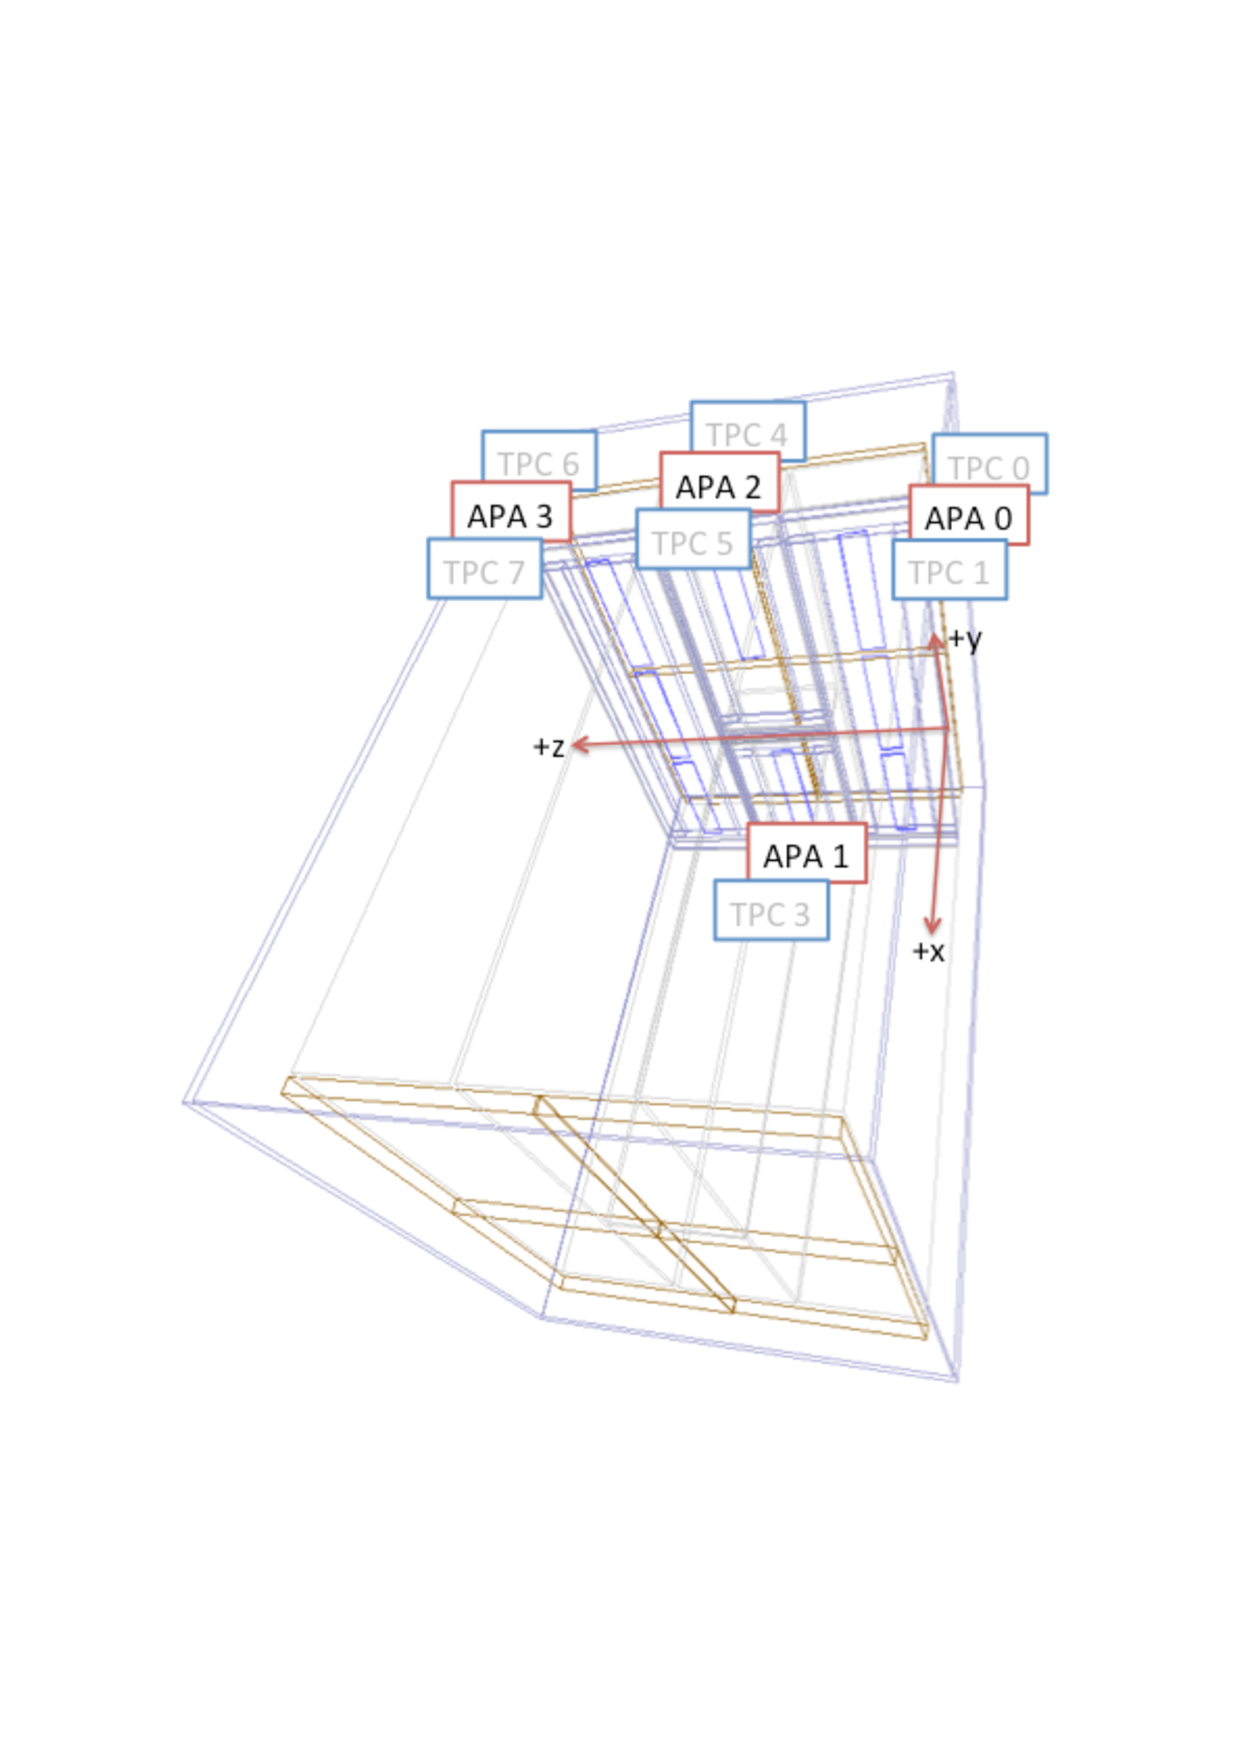
\includegraphics[width=\textwidth]{35ton_APASchem}
    \caption{The 35 ton detector coordinate system in 3D.}
  \end{subfigure}%
  \begin{subfigure}{0.48\textwidth}
    \centering
    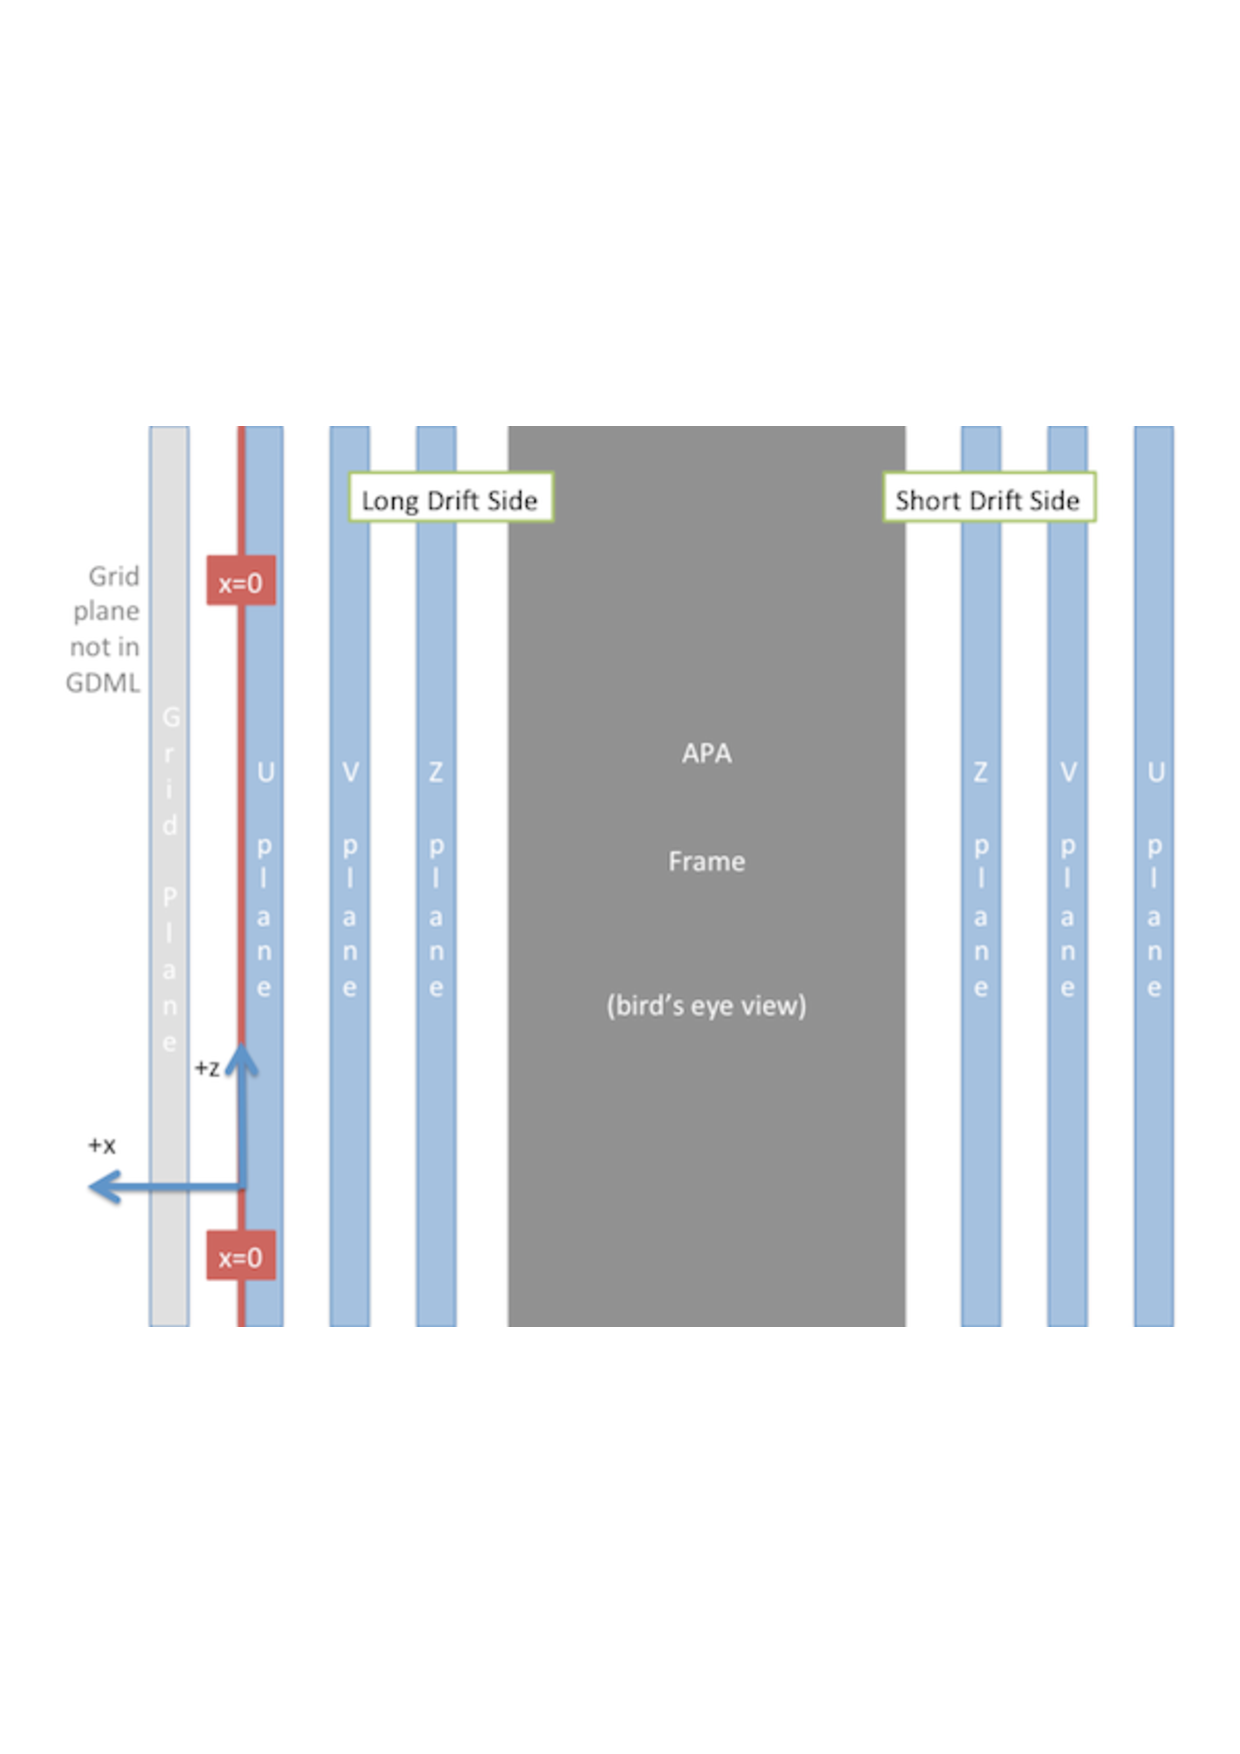
\includegraphics[width=\textwidth]{35ton_xCenter}
    \caption{The 35 ton detector coordinate system in a 2D aerial view.}
  \end{subfigure}
  \caption[The LArSoft coordinate system as it is represented in the 35 ton detector]
          {The LArSoft coordinate system as it is represented in the 35 ton detector in 3D (left) and 2D (right). The location of the origin is shown relative to the TPC detector components. Left: the four APAs (purple outlines), and eight TPCs are shown, where the even numbered TPCs are on the ``short'' drift side, 27 cm drift, and the odd numbered TPCs are on the ``long'' drift side, 223 cm drift. The CPAs (light brown outline) are also shown. Right: the location of the origin with respect to the wire planes which are wrapped around the APAs. It can be seen that $x$ = 0 is defined as the location of the U plane in the ``long'' drift volume. The figure is taken from~\citep{35tonGeomPage}.}
  \label{fig:LArSoft_coords}
\end{figure}

The simulation of particles is usually split into five processes, to reflect the different areas in which development often progresses. These stages are as follows;
\begin{itemize}
\item Particle generator.
\item Particle transport using GEANT4.
\item Full detector simulation, including detector responses. 
\item Full event reconstruction.
\item Analysis.
\end{itemize}
The advantage of separating the computational processes in this way, is that improvements can be easily applied to a file without rerunning the entire simulation/reconstruction chain. This is especially important when large Monte Carlo, or data, samples are produced for general use within the collaboration, because it allows users to concentrate on improving a specific part of the computational process. A very general analysis is performed on these all-purpose samples, which provides users with all of the Monte Carlo truth information, along with all of the reconstructed quantities. This general analysis produces a file which can be used outside of the LArSoft framework, so that users can perform analyses independently of LArSoft, should they wish to. \\

Significant focus will be given to the reconstruction of TPC data in later chapters, and so it is necessary to briefly illustrate the mechanisms by which TPC data is reconstructed in LArSoft. Much of the information presented below is summarised in~\citep{LArSoftOrg, LArSoftRecoNote}. \\

The data collected by an experiment will have detector effects such as, an electronics response function, and the digitisation of signals. The full detector simulation also introduces these detector effects into simulated data, so that the reconstruction process does not treat simulated and recorded data differently. Therefore, the first step of the reconstruction algorithms is to remove these detector effects. Once these effects are removed, the signal is estimated using the value of $signal/noise$ which would produce the measured signal. This process, called deconvolution, does not conserve pulse height, and is not guaranteed to preserve the normalisation. The deconvoluted signals are all unipolar distributions, which means that Gaussian distributions can be fitted to them, when trying to reconstruct hits. This is shown in Figure~\ref{fig:LotsOfHits}, and explained further below.\\

\begin{figure}
  \centering
  \begin{subfigure}{0.95\textwidth}
    \centering
    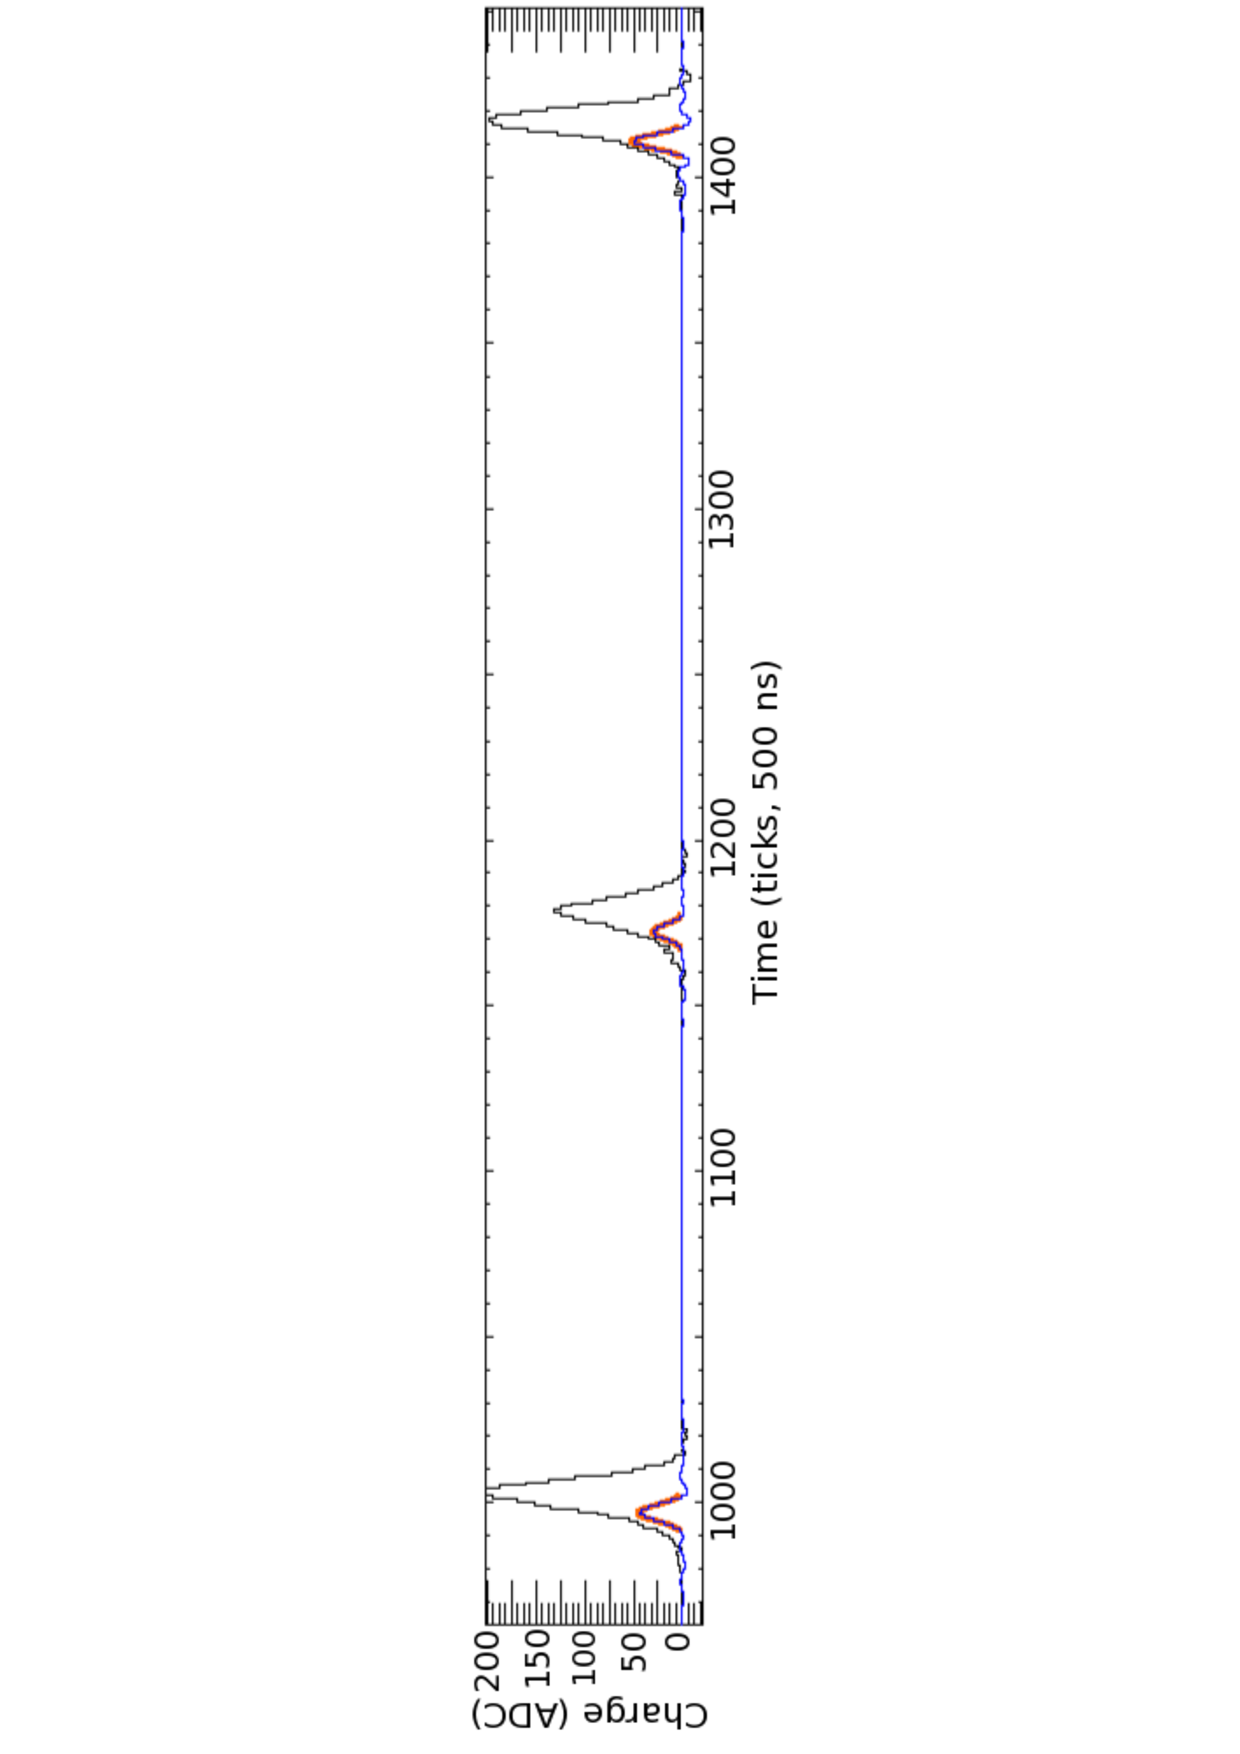
\includegraphics[width=\textwidth]{CollectionPlane}
    \caption{Collection plane depositions.}
    \label{fig:LotsOfHits_Col}
  \end{subfigure}
  \begin{subfigure}{0.95\textwidth}
    \centering
    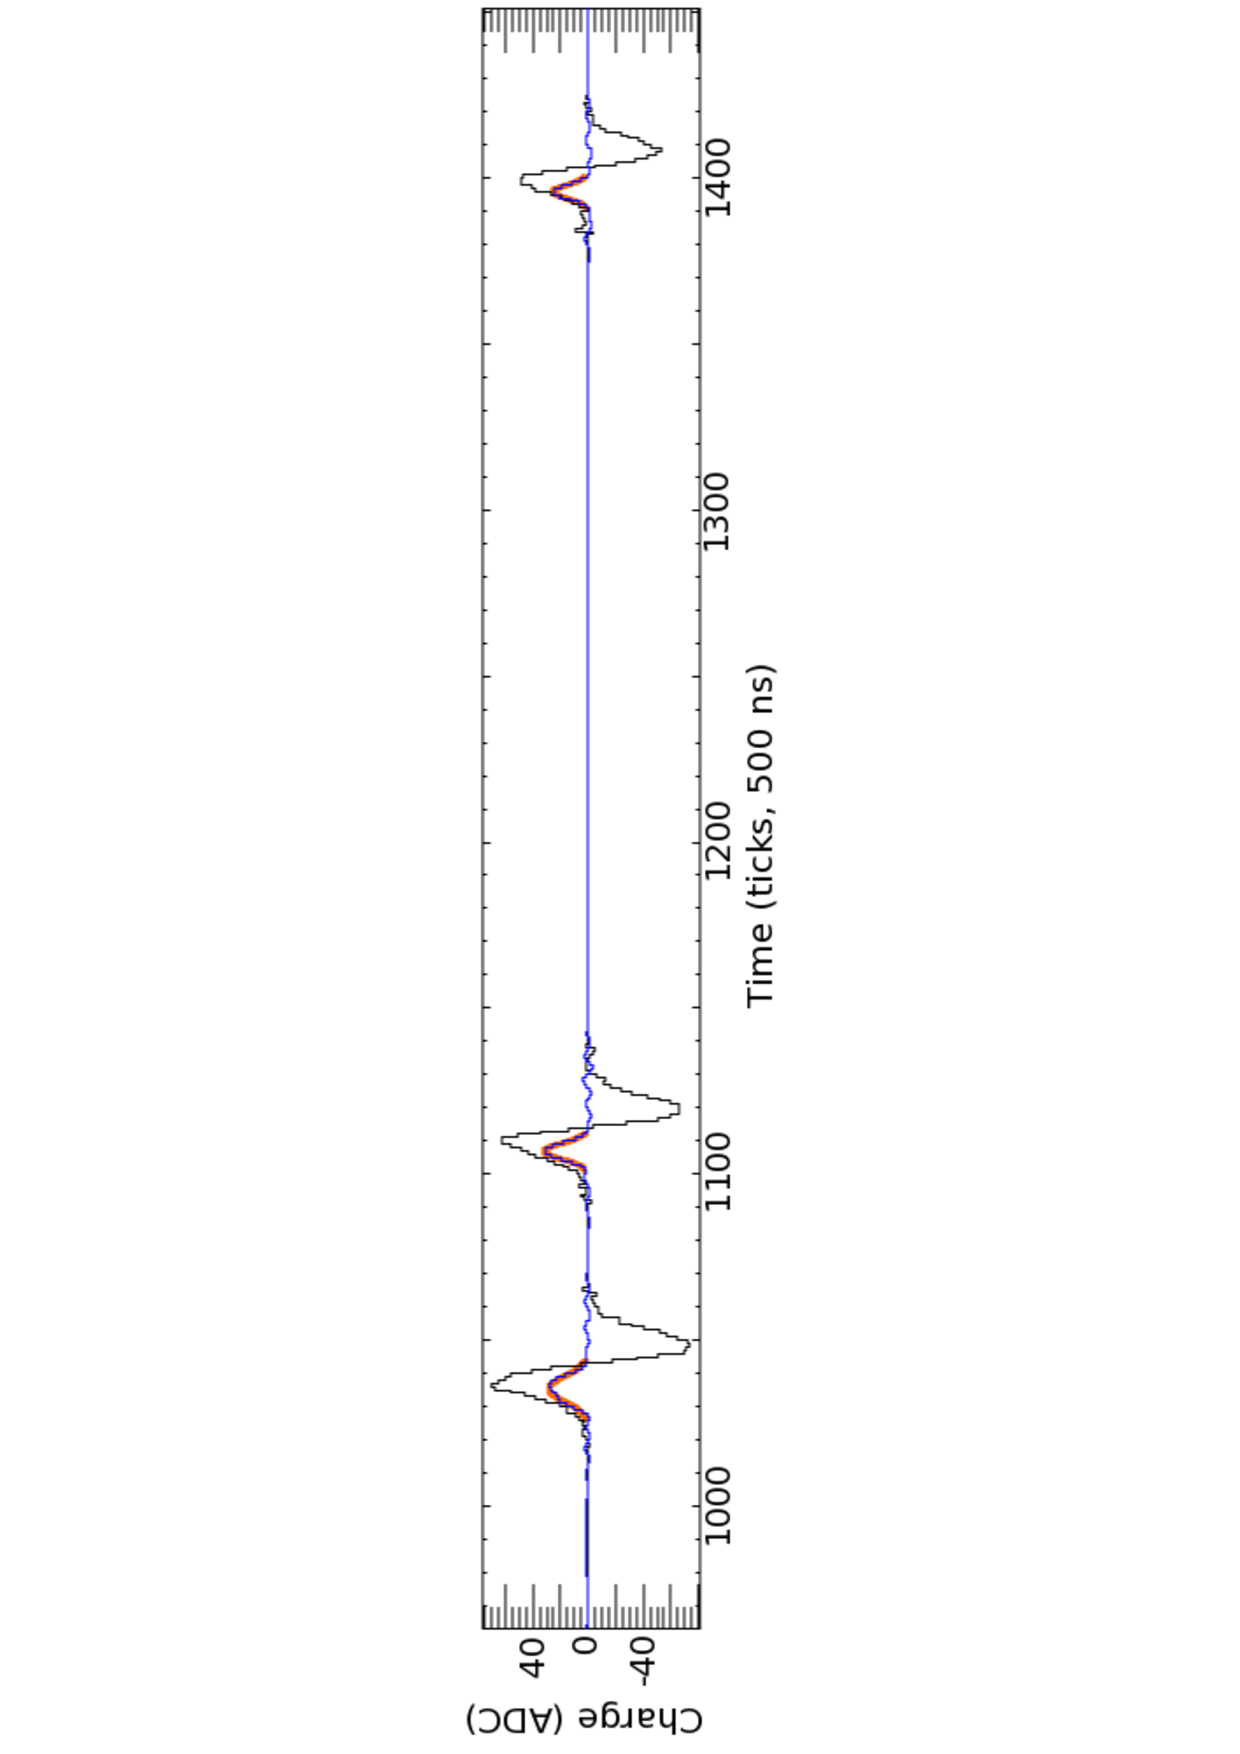
\includegraphics[width=\textwidth]{InductionPlane}
    \caption{Induction plane depositions.}
    \label{fig:LotsOfHits_Ind}
  \end{subfigure}
  \begin{subfigure}{0.95\textwidth}
    \centering
    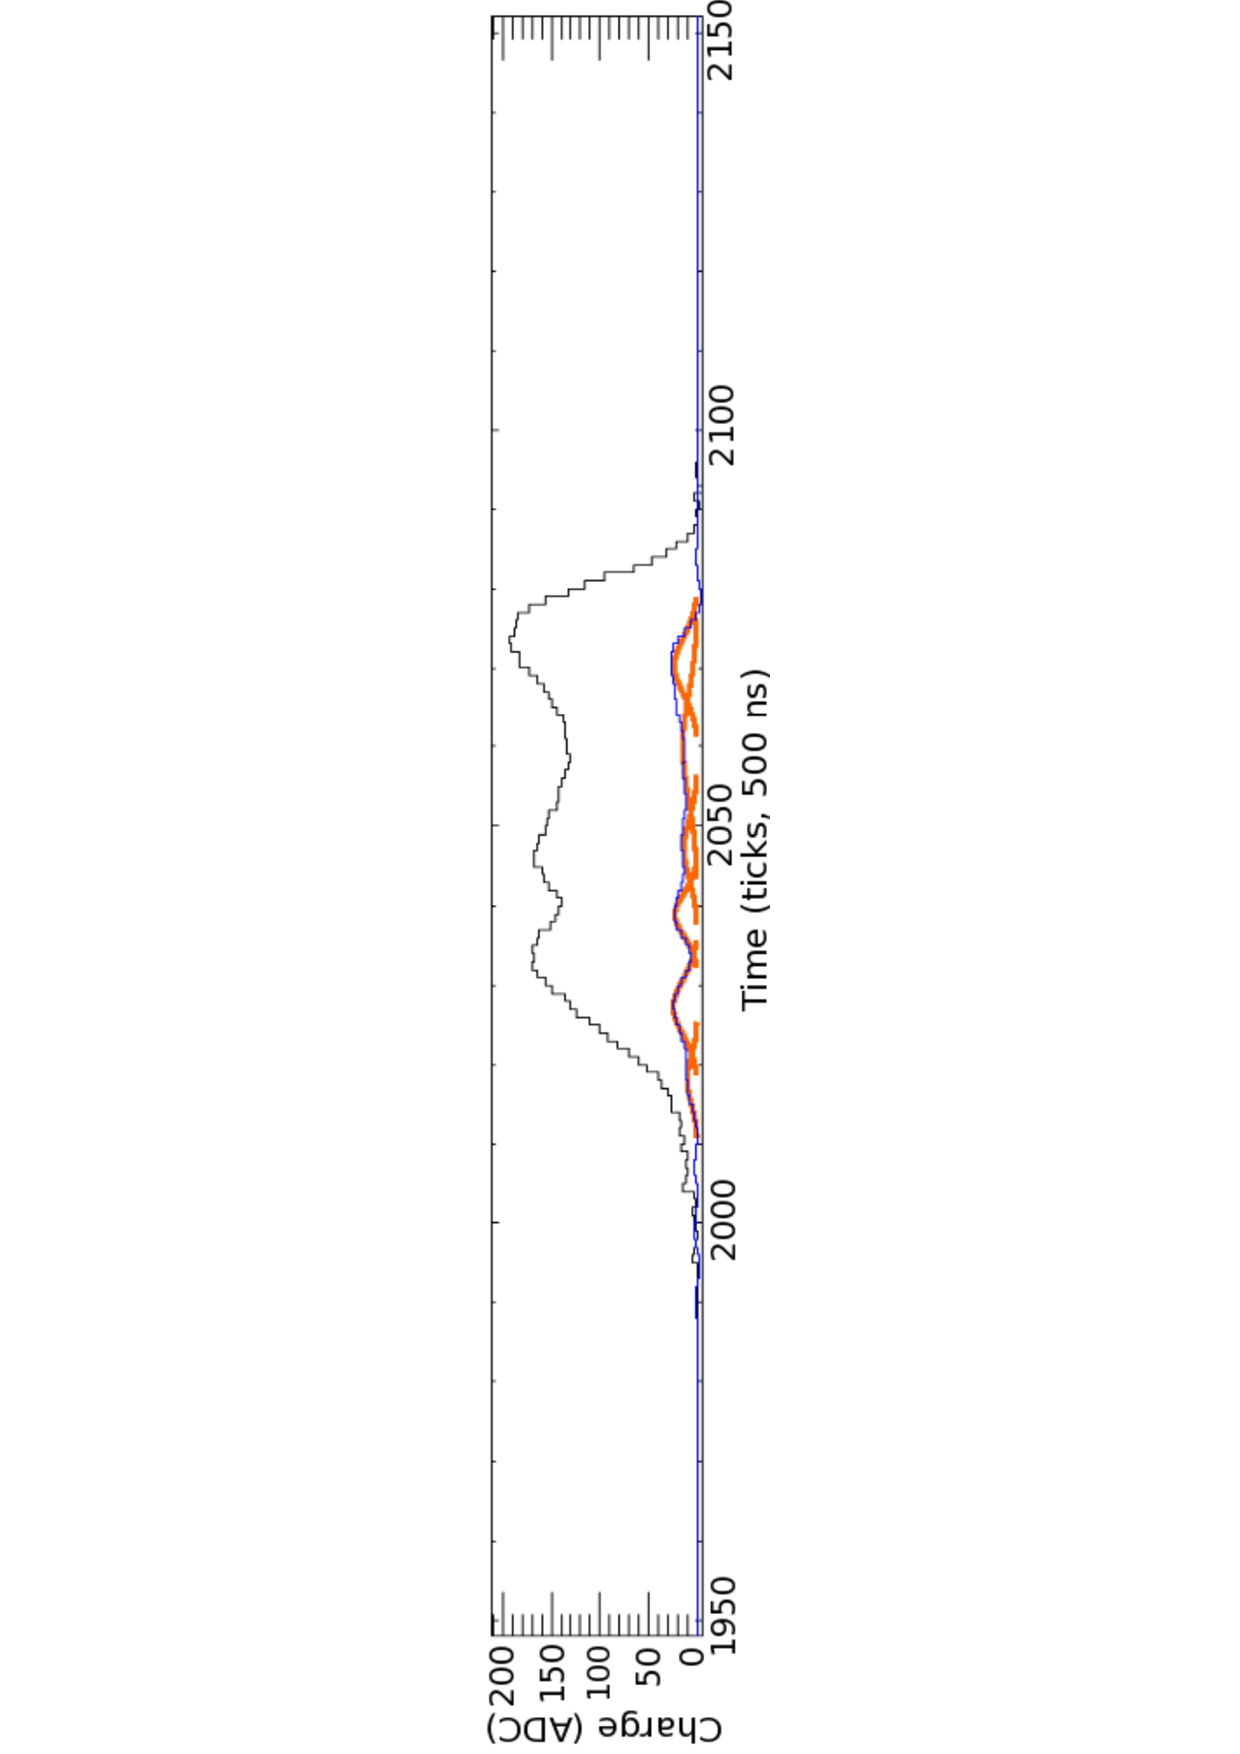
\includegraphics[width=\textwidth]{Complex}
    \caption{A large collection plane deposition over a large period of time.}
    \label{fig:LotsOfHits_Big}
  \end{subfigure}
  \caption[A selection of reconstructed hits from simulated energy depositions]
          {The raw and deconvoluted signals with reconstructed hits for simulated energy depositions. The depositions are from particles generated by CRY and are not from a single event, as such they have been selected for demonstration purposes only. The plots are shown with increasing charge (ADC) on the $y$ axis, and increasing time (ticks, 500 ns) on the $x$ axis. The black lines represent the raw signals, the blue lines represent the deconvoluted signals, and the orange lines represent the reconstructed hits. Top: depositions on a collection plane wire, it can be seen that the raw signal is unipolar. Middle: depositions on an induction plane wire, it can be seen that the raw signal is bi-polar, whilst the deconvoluted signal, and reconstructed hits, are unipolar. Bottom: a complex deposition on a collection plane wire, where multiple reconstructed hits are required to reproduce the deconvoluted signal.}
  \label{fig:LotsOfHits}
\end{figure}

The deconvoluted signals are reconstructed into hits by identifying regions that are above a threshold value, and then attempting to replicate the signal in these regions by fitting to Gaussian distributions. For isolated hits, this is typically achieved using only one Gaussian distribution, however, for large energy depositions, over a large period time, where many particles are involved, multiple Gaussian distributions are often required. Large energy depositions are also possible when the direction of the particle aligns with the inclination of a wire plane, this means that all of the deposited energy may be deposited on a single wire. Examples of reconstructed hits are shown in Figure~\ref{fig:LotsOfHits}. These figures are taken from separate events where CRY was used to generate the particles, and so do not correspond to a continuous simulated event. They have been selected only as a demonstration of the process of hit reconstruction. Figures~\ref{fig:LotsOfHits_Col}, and~\ref{fig:LotsOfHits_Ind}, show multiple time-separated energy depositions on a collection plane wire, and an induction plane wire, respectively. A more complex energy deposition on a collection plane wire is shown in Figure~\ref{fig:LotsOfHits_Big}, where energy depositions from many particles, at similar times, have created a complicated energy deposition, which requires many reconstructed hits to explain. \\

As noted in Section~\ref{sec:DUNEDetector_SP}, and Section~\ref{sec:The35tonDetector}, the DUNE FD, and the 35~ton detector, both have wrapped wires on the induction planes. Hence, the location of the reconstructed hit on an induction wire is ambiguous, as a single wire has many wire segments, as shown in Figure~\ref{fig:FDWireWrap}. An important feature of this ambiguity, is that the TPC in which an induction plane hit occurred cannot be identified, unless it is combined with another hit. These ambiguities do not extend to the collection plane wires, as they are not wrapped, and so consist of only a single wire segment, in a single TPC. Hits are combined across the three planes by identifying wire segments on each plane which intersect, and have hits at common times. In the traditional reconstruction process only hits that make these so-called ``triple points'' are considered disambiguated, with other hits being identified as noise hits, causing them to be discarded. \\

The inclination of the wire planes has to be carefully chosen so as to minimise both the number of wires required, and the number of times that wire triplets intersect. This is shown in Figure~\ref{fig:WirePitches}, where the wire inclinations used in the 35~ton detector are compared to those in the DUNE FD reference design. The inclination of induction plane wires in the 35~ton detector was 45$^{\circ}$ $\pm$ 0.7$^{\circ}$, meaning that many wire triplets cross twice, and some wire pairs cross three times. The inclination of induction plane wires in the FD reference design is 36$^{\circ}$, meaning that wire triplets only ever cross once. When wire triplets cross multiple times, the triplet which has the smallest distance between the common intersection point, and the two-wire intersection points, is chosen as the location of the hit. This is shown as the ``Good intersection'' on the right panel in Figure~\ref{fig:WirePitches}. The different wire pitches in the 35 ton detector were necessary so that one of the triple points could be evaluated to be the better candidate for the hit location, as with a wire pitch of 45$^{\circ}$ it can be impossible to distinguish between different triple points. The inclination of wires in the FD was chosen to be 36$^{\circ}$ to remove the possibility of multiple intersection points, as given the geometry of the APAs, multiple intersection points are impossible, and so disambiguation is much simpler. The lower inclination results in more induction wires being required though, making it more expensive to instrument the detector. It is also important that all wires on a given APA are either read out at the top, or base, of the APA. This is because there must be minimal space between TPCs in the DUNE FD, in order to reduce the amount of internal dead space, and reading out APAs from the sides would introduce large regions of dead space. As a result of this, APAs at the top of the cryostat are read out from the top of the APA, whilst APAs at the bottom of the cryostat are read out from the bottom of the APA. \\

\begin{figure}
  \centering
  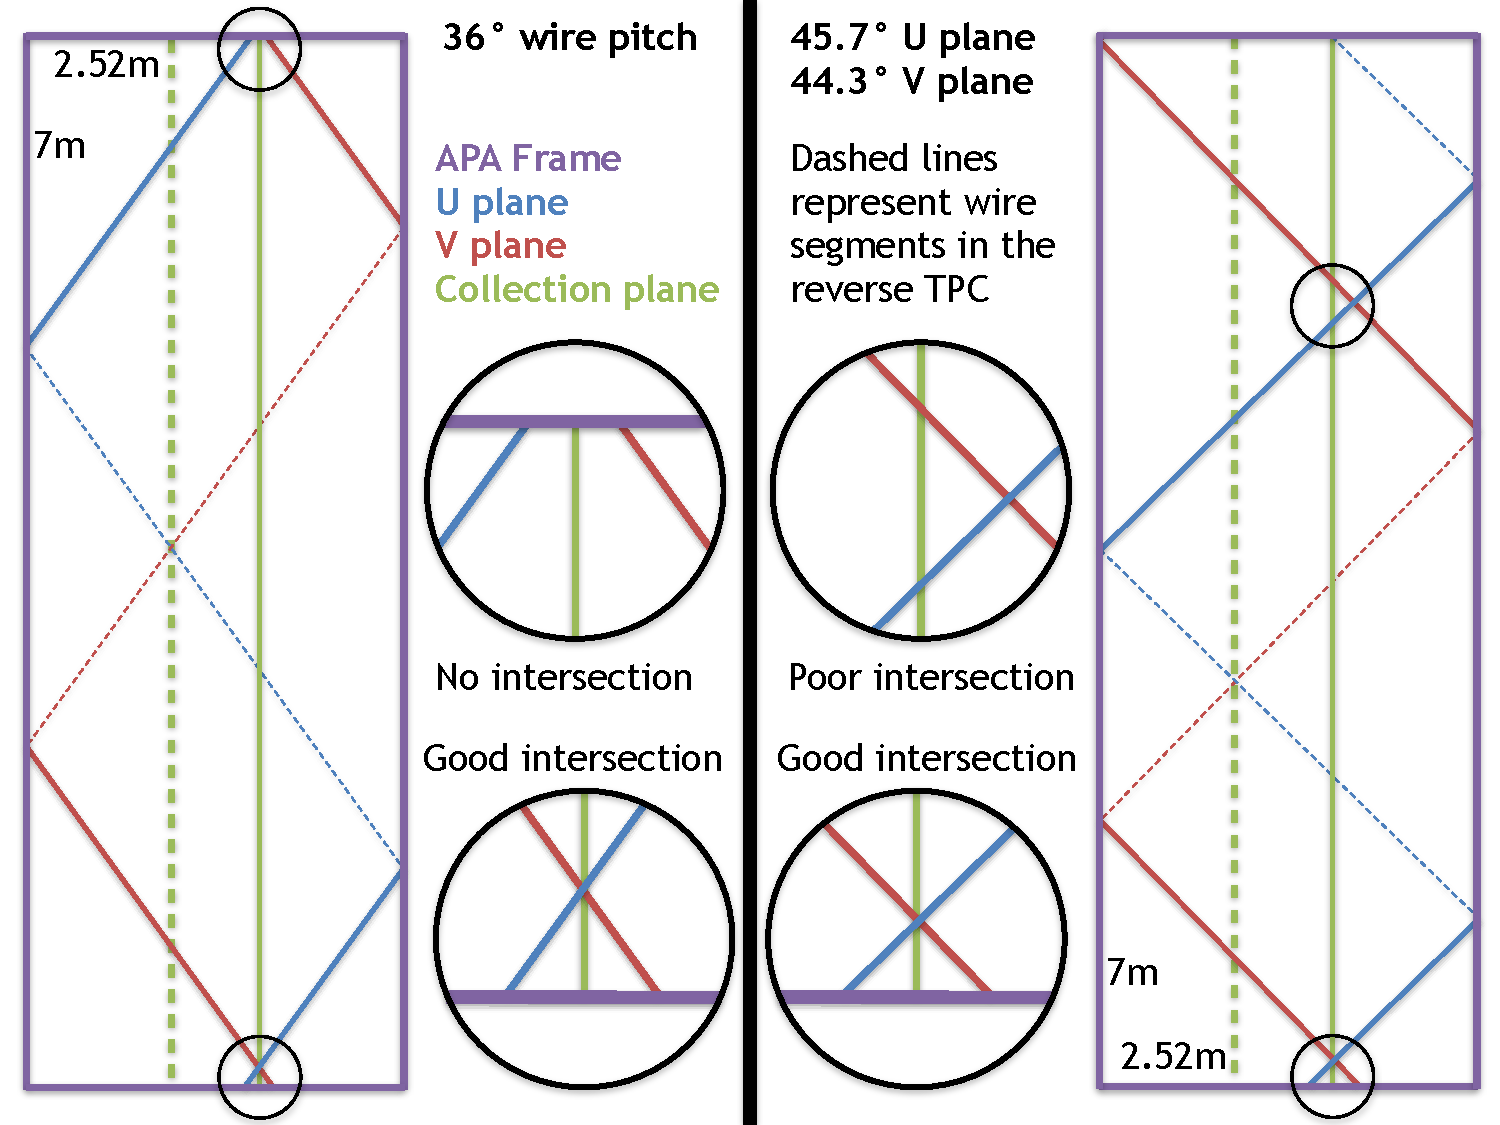
\includegraphics[width=0.85\textwidth]{WireAngleCondition}
  \caption[Performing disambiguation with different wire pitches.]
          {The effect that different wire pitches have on the ability to perform disambiguation in APAs with the far detector geometry. Left: induction plane wires with a wire pitch of 36$^{\circ}$, this is the wire pitch that is used in the FD reference design. Right: induction plane wires with a wire pitches of 45$^{\circ}$ $\pm$ 0.7$^{\circ}$, this was the wire pitch that was was used in the 35 ton detector. The left panel shows that only one ``triple point'' can be made with the three wires shown, and so disambiguation is trivial. The right panel shows that two ``triple points'' can be made with the three wires shown. The ``triple point'' where the three wires have a common intersection point is labelled as a ``good intersection,'' and it is this intersection point which would be chosen for the disambiguated hit.}
  \label{fig:WirePitches}
\end{figure}

Once the hits have been disambiguated they are combined to make clusters in each of the three planes. The clustering process is usually performed in wire-tick space on each plane separately, where all the hits from a single track or shower, should make a single cluster in each plane. It is possible to seed the start of clusters by using imaging techniques such as a Harris transform~\citep{HarrisTrans}, or to identify straight lines by using Hough transforms~\citep{HoughTrans}, though these are rarely used. As hits from a physical entity are unlikely to remain on a single channel, or all come at identical times, clusters are often spread out over many channels, for a range of times, especially when performing clustering for showers. \\

Once clusters have been identified in each plane, they can then be merged into 3-dimensional tracks and showers. The two most common tracking algorithms are PMTrack~\citep{PMTrack} and Pandora~\citep{Pandora}, and the most common showering algorithm is EMShower~\citep{EMShower}. As the tracking algorithms will be discussed in Chapters~\ref{chap:35tonSim} and~\ref{chap:35tonData}, a very brief overview of them will be given. PMTrack is a multi-trajectory fit with some capabilities of pattern recognition, it builds its outputs by looking at the projection of multiple clusters in all projections, and builds 3D objects which best represent the 2D inputs~\citep{LArSoftOrg, PMTrackJanCollab}. Pandora utilises a multi-algorithm approach to reconstruction to gradually build up a 3D picture of the event, whereby candidate vertices are identified and ranked from the initial 2D inputs~\citep{LArSoftOrg}. \\

Once 3D objects have been reconstructed, the calorimetric quantities need to be determined, this is often done separately for each plane. Two models exist for calculating $\frac{dE}{dx}$ in LArSoft, Birks model~\citep{BirksModel} and a modified Box model~\citep{PIDA_Paper}. The modified Box model uses a correction to the Box model~\citep{BoxModel} at low values of $\frac{dE}{dx}$. Normally the modified Box model is used, as it holds for both large and small ionisations, whereas Birks model experiences difficulties at large ionisations, and the traditional Box model struggles at low $\frac{dE}{dx}$. Both models incorporated in LArSoft calculate the $\frac{dE}{dx}$ of a hit using the deposited charge ($dQ$), and the track pitch ($dx$) of the hit, as well as the conversion of ADC value to number of electrons ($C_{ADC \rightarrow e^{-}}$), the conversion of GeV to number of electrons ($C_{GeV \rightarrow e^{-}}$), a correction due to the electron lifetime ($C_{lifetime}$), the LAr density ($\rho$), the electric field ($E_{field}$), and the tuneable electron recombination factors ($Recomb_{A/B}$). The series of equations used in Birks model are shown in Equation~\ref{eq:Birks}, whilst those used in the modified Box model are shown in Equation~\ref{eq:ModBox}. \\

\begin{subequations}
  \label{eq:Birks}
  \begin{align}
    \frac{dE}{dx} &= \frac{ (dQ/dx)_{Cor} }{ \alpha - [\beta \times (dQ/dx)_{Cor} ] } \label{eq:Birks_1} \\
    (dQ/dx)_{Cor} &= \frac{dQ}{dx} \times \frac{ C_{lifetime} }{ C_{ADC \rightarrow e^{-}} } \label{eq:Birks_Correc} \\
    \alpha &= Recomb_{A} \times C_{GeV \rightarrow e^{-}} \times 10^{-3} \label{eq:Birks_A}\\
    \beta  &= \frac{ Recomb_{B} }{ \rho \times E_{field} } \label{eq:Birks_B}
  \end{align}
\end{subequations}

\begin{subequations}
  \label{eq:ModBox}
  \begin{align}
    \frac{dE}{dx} &= \frac{ e^{\alpha} - Recomb_{A} }{ \beta } \label{eq:ModBox_1} \\
    \alpha &= \frac{10^3 \times \beta }{ C_{GeV \rightarrow e^{-} } } \times (dQ/dx)_{Cor} \label{eq:ModBox_A}\\
    (dQ/dx)_{Cor} &= \frac{dQ}{dx} \times \frac{ C_{lifetime} }{ C_{ADC \rightarrow e^{-}} } \label{eq:ModBox_Correc} \\
    \beta &= \frac{ Recomb_{B} }{ \rho \times E_{field} } \label{eq:ModBox_B}
  \end{align}
\end{subequations}

When performing calorimetry, it is also important that the interaction time is known, so that the $x$ positions of hits can be corrected, as they will initially be reconstructed assuming an interaction time of 0 s. This assumption is made because the beam trigger is placed at a time of $T = 0$ when considering beam induced events. An unknown interaction time causes the hit and track positions to be calculated incorrectly. \textcolor{red}{The correction to the reconstructed positions has to be made by hand, as the positions of the reconstructed hits cannot be modified in the event record.}
